\documentclass[12pt,initial,twoside,maitrise]{dms}
\usepackage[utf8]{inputenc} %Obligatoires
%\usepackage[T1]{fontenc}    %
\usepackage[dvipsnames]{xcolor}
\usepackage{array}
\usepackage{algorithmicx}
\usepackage{algorithm}
\usepackage{algpseudocode}
\usepackage{amsmath}
\usepackage{rail}
\usepackage{graphicx}

\usepackage[hidelinks]{hyperref}
\hypersetup{
    colorlinks,
    linkcolor={red!50!black},
    citecolor={blue!50!black},
    urlcolor={blue!80!black}
}

\renewcommand{\UrlFont}{\rmfamily}

\usepackage{bm}

\usepackage{natbib}

\usepackage{enumitem}
\usepackage{graphviz}
\usepackage{epstopdf}
\usepackage{auto-pst-pdf}

% Quotes
\usepackage{epigraph}
\beforeepigraphskip=-20pt
\afterepigraphskip=20pt
\renewcommand{\textflush}{flushepinormal}

% Trees
\usepackage{tikz}
\usepackage{tikz-qtree}

% Table Checks
\usepackage{booktabs}
\usepackage{pifont}
\usepackage{fontawesome}
\usepackage{float}

\newcommand{\wmark}{\textcolor{orange}{\ding{45}}}
\newcommand{\cmark}{\textcolor{green!80!black}{\ding{51}}}
\newcommand{\xmark}{\textcolor{red}{\ding{55}}}

\usepackage{multicol}
\newlist{todolist}{itemize}{2}
\setlist[todolist]{label=$\square$}
\newcommand{\done}{\rlap{$\square$}{\raisebox{2pt}{\large\hspace{1pt}\cmark}}%
\hspace{-2.5pt}}

\newcommand{\argmax}[1]{\underset{#1}{\operatorname{arg}\,\operatorname{max}}\;}
\newcommand{\argmin}[1]{\underset{#1}{\operatorname{arg}\,\operatorname{min}}\;}

% Table
\newcommand*\rot{\rotatebox{90}}

\usepackage{menukeys}
\usepackage{relsize}

% Code listings
%\usepackage[scaled]{beramono}
\usepackage{fontspec}
\setmonofont{JetBrains Mono}
\usepackage{ocr}
\usepackage[T1]{fontenc}
\usepackage[skins,breakable,listings]{tcolorbox}

\usepackage{accsupp}
\newcommand{\noncopyable}[1]{%
    \BeginAccSupp{method=escape,ActualText={}}%
    #1%
    \EndAccSupp{}%
}

\lstdefinelanguage{kotlin}{
    comment=[l]{//},
    commentstyle={\color{gray}\ttfamily},
    emph={delegate, filter, firstOrNull, forEach, it, lazy, mapNotNull, println, repeat, assert, with, head, tail, len, return@},
    numberstyle=\noncopyable,
    emphstyle={\color{OrangeRed}},
    identifierstyle=\color{black},
    keywords={abstract, actual, as, as?, break, by, class, companion, continue, data, do, dynamic, else, enum, expect, false, final, for, fun, get, if, import, in, infix, interface, internal, is, null, object, open, operator, override, package, private, public, return, sealed, set, super, suspend, this, throw, true, try, typealias, val, var, vararg, when, where, while, tailrec, reified},
    keywordstyle={\color{NavyBlue}\bfseries},
    morecomment=[s]{/*}{*/},
    morestring=[b]",
    morestring=[s]{"""*}{*"""},
    ndkeywords={@Deprecated, @JvmField, @JvmName, @JvmOverloads, @JvmStatic, @JvmSynthetic, Array, Byte, Double, Float, Boolean, Int, Integer, Iterable, Long, Runnable, Short, String},
    ndkeywordstyle={\color{BurntOrange}\bfseries},
    sensitive=true,
    stringstyle={\color{ForestGreen}\ttfamily},
    literate={`}{{\char0}}1
}

\lstdefinelanguage{docker}{
    keywords={FROM, RUN, COPY, ADD, ENTRYPOINT, CMD,  ENV, ARG, WORKDIR, EXPOSE, LABEL, USER, VOLUME, STOPSIGNAL, ONBUILD, MAINTAINER},
    keywordstyle=\color{blue}\bfseries,
    numberstyle=\noncopyable,
    identifierstyle=\color{black},
    sensitive=true,
    comment=[l]{\#},
    commentstyle=\color{purple}\ttfamily,
    stringstyle=\color{red}\ttfamily,
    morestring=[b]',
    morestring=[b]"
}

\lstdefinelanguage{BashPrompt}{%
    keywordstyle=\color{blue},
    basicstyle=\ttfamily,
    literate={\$}{{\bfseries\textcolor{blue}{\noncopyable\$}}}1
    {~}{{\bfseries\textcolor{blue}{\noncopyable\textasciitilde}}}1,
}

\lstdefinelanguage{DtsPrompt}{%
    keywordstyle=\color{blue},
    basicstyle=\ttfamily,
    literate={dt> }{{\bfseries\textcolor{blue}{\noncopyable{dt> }}}}1
}

\lstdefinelanguage{XML}{
    basicstyle=\ttfamily,
    numberstyle=\noncopyable,
    morestring=[s][\color{black}]{"}{"},
    morestring=[s][\color{black}]{>}{<},
    stringstyle=\color{black},
    identifierstyle=\color{blue}\bfseries,
    moreidentifier={launch, node},
    keywordstyle=\color{brown},
    morekeywords={name, pkg, type, output},
}

\lstdefinelanguage{bnf}{
    comment=[l]{//},
    commentstyle={\color{gray}\ttfamily},
    numberstyle=\noncopyable,
    basicstyle=\ttfamily,
    morestring=[s][\color{RoyalPurple}\bfseries]{"}{"},
    emphstyle={\color{ForestGreen}\bfseries},
    moreemph={TYPE, FIELD, SEPARATOR, CONSTANT, COMMENT},
    identifierstyle=\color{blue}\bfseries,
    keywordstyle={\color{NavyBlue}\bfseries},
    morekeywords={property, recover_property, rosInterfaceFile},
    ndkeywords={getType, get Key, getValue, getName, setName, getNameIdentifier},
    ndkeywordstyle={\color{black}\itshape},
}

%% Adjustments

\lstdefinestyle{barelisting}{
    language=kotlin,
    basicstyle=\ttfamily\scriptsize,
    numberstyle=\footnotesize\noncopyable,
    backgroundcolor=\color{slightgray},
    frame=single,
    tabsize=2,
    rulecolor=\color{black!30},
    breaklines=true,
    inputencoding=utf8
}

\usepackage{lipsum}
\tcbuselibrary{listings,breakable}

\newtcblisting{unbreakablekotlin}[1][]{%
    breakable=false,
    listing only,
    boxsep=-1.5pt,
    top=-1pt,
    bottom=-0.5pt,
    listing options={
        language=kotlin,
        basicstyle=\ttfamily\footnotesize,
        numberstyle=\footnotesize\noncopyable,
        tabsize=2,
        numbers=right,
        breaklines=true,
        inputencoding=utf8,
        escapeinside={(*}{*)},
        #1
    },
    underlay={
        \path[draw=none] (interior.north west) rectangle node[white]{\includegraphics[width=5mm]{../figures/kotlin_file.png}} ([xshift=-10mm,yshift=-10mm]interior.north west);
    }
}

\newtcblisting{kotlinlisting}[1][]{%
    listing options={
        language=kotlin,
        basicstyle=\ttfamily\tiny,
        numberstyle=\footnotesize\noncopyable,
        showstringspaces=false,
        tabsize=2,
        breaklines=true,
        numbers=right,
        inputencoding=utf8,
        escapeinside={(*}{*)},
        #1
    },
    underlay unbroken and first={%
        \path[draw=none] (interior.north west) rectangle node[white]{\includegraphics[width=4mm]{../figures/kotlin_file.png}} ([xshift=-10mm,yshift=-10mm]interior.north west);
    }
}

\newtcblisting{pclisting}[1][]{%
    listing options={
        language=BashPrompt,
        basicstyle=\ttfamily\footnotesize,
        numberstyle=\noncopyable,
        tabsize=2,
        numbers=right,
        inputencoding=utf8,
        escapeinside={(*}{*)},
        #1
    },
    underlay unbroken and first={%
        \path[draw=none] (interior.north west) rectangle node[white]{\includegraphics[width=5mm]{../figures/laptop_icon.png}} ([xshift=-10mm,yshift=-10mm]interior.north west);
    }
}

\newtcblisting{flexlisting}[1][]{%
    left=20pt,
    listing options={
        language=DtsPrompt,
        basicstyle=\ttfamily\footnotesize,
        numberstyle=\noncopyable,
        numbers=right,
        tabsize=2,
        inputencoding=utf8,
        #1
    }
}

\newtcblisting{dtslisting}[1][]{%
    left=20pt,
    listing options={
        language=DtsPrompt,
        basicstyle=\ttfamily\footnotesize,
        tabsize=2,
        inputencoding=utf8,
        #1
    },
    underlay unbroken and first={%
        \path[draw=none] (interior.north west) rectangle node[white]{\includegraphics[width=6mm]{../figures/duckietown.png}} ([xshift=-10mm,yshift=-10mm]interior.north west);
    }
}

% Imitate syntax error
\usepackage{ulem}
\makeatletter
\def\uwave{\bgroup \markoverwith{\lower3.5\p@\hbox{\sixly \textcolor{red}{\char58}}}\ULon}
\font\sixly=lasy6 % does not re-load if already loaded, so no memory problem.
\makeatother

\newtcblisting{launchlisting}[1][]{%
    #1,
    listing options={
        language=XML,
        basicstyle=\ttfamily\footnotesize,
        numberstyle=\footnotesize\noncopyable,
        tabsize=2,
        numbers=right,
        breaklines=true,
        inputencoding=utf8,
        escapeinside={(*}{*)}
    },
    fonttitle=\ttfamily\small,
    underlay unbroken and first={%
        \path[draw=none] (interior.north west) rectangle node[white]{\includegraphics[width=5mm]{../figures/launch_icon.png}} ([xshift=-10mm,yshift=-9mm]interior.north west);
    }
}

\newtcblisting{dockerlisting}[1][]{%
    listing options={
        language=docker,
        basicstyle=\ttfamily\footnotesize,
        numberstyle=\footnotesize\noncopyable,
        tabsize=2,
        numbers=right,
        breaklines=true,
        inputencoding=utf8,
        escapeinside={(*}{*)}
    },
    underlay unbroken and first={%
        \path[draw=none] (interior.north west) rectangle node[white]{\includegraphics[width=6mm]{../figures/docker_icon.jpg}} ([xshift=-10mm,yshift=-9mm]interior.north west);
    }
}

\newtcblisting{bnflisting}[1][]{%
    #1,
    listing options={
        language=bnf,
        basicstyle=\ttfamily\footnotesize,
        numberstyle=\noncopyable,
        breaklines=true,
        numbers=right,
        showstringspaces=false,
    },
    fonttitle=\ttfamily\small,
    underlay unbroken and first={%
        \path[draw=none] (interior.north west) rectangle node[white]{\includegraphics[width=5mm]{../figures/bnf_file.png}} ([xshift=-10mm,yshift=-10mm]interior.north west);
    }
}

\newtcblisting{pythonlisting}[1][]{%
    #1,
    listing options={
        language=Python,
        basicstyle=\ttfamily\footnotesize,
        numberstyle=\noncopyable,
        breaklines=true,
        numbers=right,
        showstringspaces=false,
        keywordstyle=\color{blue}\bfseries,
        escapeinside={(*}{*)}
    },
    fonttitle=\ttfamily\small,
    underlay unbroken and first={%
        \path[draw=none] (interior.north west) rectangle node[white]{\includegraphics[width=5mm]{../figures/python_icon.png}} ([xshift=-10mm,yshift=-10mm]interior.north west);
    }
}

\newtcblisting{rpilisting}[1][]{%
    listing options={
        language=BashPrompt,
        basicstyle=\ttfamily\footnotesize,
        numberstyle=\noncopyable,
        tabsize=2,
        inputencoding=utf8,
        #1
    },
    underlay unbroken and first={%
        \path[draw=none] (interior.north west) rectangle node[white]{\includegraphics[width=8mm]{../figures/raspi_icon.png}} ([xshift=-10mm,yshift=-10mm]interior.north west);
    }
}

\tcbset{
    enhanced jigsaw,
    breakable,
    listing only,
    boxsep=-1pt,
    top=-1pt,
    bottom=-0.5pt,
    right=-0.5pt,
    overlay first={
        \node[black!50] (S) at (frame.south) {\Large\ding{34}};
        \draw[dashed,black!50] (frame.south west) -- (S) -- (frame.south east);
    },
    overlay middle={
        \node[black!50] (S) at (frame.south) {\Large\ding{34}};
        \draw[dashed,black!50] (frame.south west) -- (S) -- (frame.south east);
        \node[black!50] (S) at (frame.north) {\Large\ding{34}};
        \draw[dashed,black!50] (frame.north west) -- (S) -- (frame.north east);
    },
    overlay last={
        \node[black!50] (S) at (frame.north) {\Large\ding{34}};
        \draw[dashed,black!50] (frame.north west) -- (S) -- (frame.north east);
    },
    before={\par\vspace{10pt}},
    after={\par\vspace{\parskip}\noindent}
}

\newcommand*{\inlineimg}[1]{%
    \raisebox{-.3\baselineskip}{%
        \includegraphics[
            height=\baselineskip,
            width=\baselineskip,
            keepaspectratio,
        ]{#1}%
    }%
}

\definecolor{slightgray}{rgb}{0.90, 0.90, 0.90}

\usepackage{soul}
\makeatletter
\def\SOUL@hlpreamble{%
    \setul{}{3.0ex}%
    \let\SOUL@stcolor\SOUL@hlcolor%
    \SOUL@stpreamble%
}
\makeatother

\newcommand{\inline}[1]{%
    \begingroup%
    \sethlcolor{slightgray}%
    \hl{\ttfamily\footnotesize #1}%
    \endgroup
}

\newcommand{\tinline}[1]{%
    \begingroup%
    \sethlcolor{slightgray}%
    \hl{\ttfamily\tiny #1}%
    \endgroup
}


% Downloads Table
\usepackage{pgfplots}
\newcounter{marknumber}
\pgfplotsset{
    error bars/every nth mark/.style={
        /pgfplots/error bars/draw error bar/.prefix code={
            \pgfmathtruncatemacro\marknumbercheck{mod(floor(\themarknumber/2),#1)}
            \ifnum\marknumbercheck=0
            \else
            \begin{scope}[opacity=0]
                \fi
        },
        /pgfplots/error bars/draw error bar/.append code={
            \ifnum\marknumbercheck=0
            \else
\end{scope}
\fi
\stepcounter{marknumber}
}
},
scaled y ticks=false
}
\usepackage{filecontents}
\usetikzlibrary{pgfplots.dateplot}

%% Packages utiles.
\usepackage{amssymb,subfigure,icomma}
\usepackage[labelfont=bf, width=\linewidth]{caption}

\def\chapterautorefname{Chapter}
\renewcommand{\sectionautorefname}{\S}
\renewcommand{\subsectionautorefname}{\S}
\newcommand{\algorithmautorefname}{Algorithm}
\usepackage{hypcap}
\usepackage{bookmark}

\newtheorem{cor}{\corollaryname}[section]
\newtheorem{deff}[cor]{\definitionname}
\newtheorem{ex}[cor]{\examplename}
\newtheorem{lem}[cor]{\lemmaname}
\newtheorem{prop}[cor]{Proposition}
\newtheorem{rem}[cor]{\remarkname}
\newtheorem{theo}[cor]{\theoremname}

\numberwithin{equation}{section}
\numberwithin{table}{chapter}
\numberwithin{figure}{chapter}

\renewcommand{\baselinestretch}{1.5}

%\AtBeginDocument{\hypersetup{pdfborderstyle={/S/S/W 1}}}
\begin{document}

\version{1}

\title{Programming tools for intelligent systems}

\author{Breandan Considine}

\copyrightyear{2019}

\department{D\'epartement d'informatique et de recherche op\'erationnelle}

\president{Marc Feeley}

\directeur{Liam Paull}

\codirecteur{Michalis Famelis}

\membrejury{Eug\`ene Syriani}

\dateacceptation{La date d'acceptation}

%% Voici les disciplines possibles (voir avec votre directeur):
%% \sujet{statistique},
%% \sujet{mathématiques}, \orientation{mathématiques appliquées},
%% \orientation{mathématiques fondamentales}
%% \orientation{mathématiques de l'ingénieur} et
%% \orientation{mathématiques appliquées}

\sujet{Informatique}

%%
%% Fin des variables à définir. La commande \maketitle créera votre
%% page titre.

\pagenumbering{roman}
\maketitle
\maketitle

% Pour générer la deuxième page titre, il faut appeler à nouveau \maketitle
% Cette page est optionnelle et son inclusion est laissé à la discrétion
% de l'étudiant et du directeur de recherche, ou de tout autre instance
% d'autorité.

%%------------------------------------------------- %
%%              pages iv                            %
%%------------------------------------------------- %
\anglais

\ProvidesPackage{preamble}

\usepackage{url}
\usepackage{array}
\usepackage{amsmath,amssymb,amsfonts,textcomp,amsthm}
\usepackage{booktabs}
\usepackage{relsize}
\usepackage{nicefrac}
\usepackage{graphicx}
\usepackage{rotating}
\usepackage{nth}
\usepackage{acronym}
\usepackage{bm}
%\usepackage{caption} \DeclareCaptionType{copyrightbox}
\usepackage{footnote}
\usepackage{color}



\usepackage{array}
\usepackage{tabularx}
\newcolumntype{x}[1]{>{\centering\arraybackslash\hspace{0pt}}m{#1}}
\newcommand{\tabbox}[1]{#1}

\usepackage{hyperref}
\definecolor{mydarkblue}{rgb}{0,0.08,0.45}
\hypersetup{
pdftitle={},
pdfauthor={},
pdfsubject={},
pdfkeywords={},
pdfborder=0 0 0,
pdfpagemode=UseNone,
colorlinks=true,
linkcolor=mydarkblue,
citecolor=mydarkblue,
filecolor=mydarkblue,
urlcolor=mydarkblue,
pdfview=FitH}

\newcommand{\asdf}{$^{\textnormal{th}}$}

\newcommand{\binarysum}{\sum_{\bf{x} \in \{0,1\}^D}}
\newcommand{\expect}{\mathbb{E}}
\newcommand{\expectargs}[2]{\mathbb{E}_{#1} \left[ {#2} \right]}
\newcommand{\var}{\mathbb{V}}
\newcommand{\varianceargs}[2]{\mathbb{V}_{#1} \left[ {#2} \right]}
\newcommand{\variance}{\mathbb{V}}
\newcommand{\cov}{\operatorname{cov}}
\newcommand{\Cov}{\operatorname{Cov}}
\newcommand{\covarianceargs}[2]{\Cov_{#1} \left[ {#2} \right]}
\newcommand{\colvec}[2]{\left[ \begin{array}{c} {#1} \\ {#2} \end{array} \right]}
\newcommand{\tbtmat}[4]{\left[ \begin{array}{cc} {#1} & {#2} \\ {#3} & {#4} \end{array} \right]}

%\newcommand{\covskinny}[2]{\var\!\left(#1\middle\vert#2\right)}

\newcommand{\acro}[1]{\textsc{#1}}
%\newcommand{\vect}[1]{\boldsymbol{#1}}
%\newcommand{\vect}[1]{{\bf{#1}}}
\newcommand{\mat}[1]{\mathbf{#1}}
\newcommand{\pderiv}[2]{\frac{\partial #1}{\partial #2}}
\newcommand{\npderiv}[2]{\nicefrac{\partial #1}{\partial #2}}

\newcommand{\pha}{^{\phantom{:}}}

\newcommand{\argmin}{\operatornamewithlimits{argmin}}
\newcommand{\argmax}{\operatornamewithlimits{argmax}}

% The following designed for probabilities with long arguments

\newcommand{\Prob}[2]{P\!\left(\,#1\;\middle\vert\;#2\,\right)}
\newcommand{\ProbF}[3]{P\!\left(\,#1\!=\!#2\;\middle\vert\;#3\,\right)}
\newcommand{\p}[2]{p\!\left(#1\middle\vert#2\right)}
\newcommand{\po}[1]{p\!\left(#1\right)}
\newcommand{\pF}[3]{p\!\left(\,#1\!=\!#2\;\middle\vert\;#3\,\right)}
\newcommand{\mean}[2]{{m}\!\left(#1\middle\vert#2\right)}
%\newcommand{\novmean}[2]{{m}\!\left(#1\middle\vert#2\right)}
%\newcommand{\novcov}[2]{\var\!\left(#1\middle\vert#2\right)}
%\newcommand{\cov}[2]{\var\!\left(#1\middle\vert#2\right)}
%\newcommand{\pskinny}[2]{p\!\left(#1\;\middle\vert\;#2\right)}
%\newcommand{\meanskinny}[2]{{m}\!\left(#1\middle\vert#2\right)}
%\newcommand{\covskinny}[2]{\var\!\left(#1\middle\vert#2\right)}

\newcommand{\vI}{\mat{I}}
\newcommand{\vX}{\mat{X}}
\newcommand{\vY}{\mat{Y}}
\newcommand{\vZ}{\mat{Z}}
\newcommand{\vK}{\mat{K}}
\newcommand{\vs}{\vect{s}}
\newcommand{\va}{\vect{a}}
\newcommand{\vA}{\vect{A}}
\newcommand{\vb}{\vect{b}}
\newcommand{\vB}{\mat{B}}
\newcommand{\vr}{\vect{R}}
\newcommand{\vR}{\mat{R}}
\newcommand{\vS}{\mat{S}}
\newcommand{\vu}{\vect{u}}
\newcommand{\vh}{\vect{h}}
\newcommand{\vk}{\vect{k}}
\newcommand{\vc}{\vect{c}}
\newcommand{\vC}{\mat{C}}
\newcommand{\vw}{\vect{w}}
\newcommand{\vx}{\vect{x}}
\newcommand{\vy}{\vect{y}}
\newcommand{\vz}{\vect{z}}
\newcommand{\vmu}{\vect{\mu}}
\newcommand{\vpi}{\vect{\pi}}
\newcommand{\vphi}{\vect{\phi}}
\newcommand{\vSigma}{\mat{\Sigma}}
\newcommand{\vtheta}{\vect{\theta}}
\newcommand{\vl}{\vect{l}}
\newcommand{\vq}{\vect{q}}
\newcommand{\vf}{\vecf}
\newcommand{\vg}{\vect{g}}
\newcommand{\vell}{\vect{\ell}}
\newcommand{\ve}{\vect{\epsilon}}
\newcommand{\vzero}{\vect{0}}
\newcommand{\vone}{\vect{1}}
\newcommand{\vecf}{\boldsymbol{f}}
\newcommand{\vect}[1]{\mathbf{#1}}

\newcommand{\He}{\mathcal{H}}
\newcommand{\normx}[2]{\left\|#1\right\|_{#2}}
\newcommand{\Hnorm}[1]{\normx{#1}{\He}}
\newcommand{\mmd}{{\rm MMD}}


\newcommand{\mf}{\bar{\vf}}

\newcommand{\st}{_\star}

\newcommand{\inv}{^{{\mathsmaller{-1}}}}
\newcommand{\tohalf}{^{{\mathsmaller{\nicefrac{1}{2}}}}}

\newcommand{\Normal}{\mathcal{N}}
\newcommand{\N}[3]{\mathcal{N}\!\left(#1|#2,#3\right)}
\newcommand{\Nt}[2]{\mathcal{N}\!\left(#1,#2\right)}
\newcommand{\bN}[3]{\mathcal{N}\big(#1|#2,#3\big)}
\newcommand{\boldN}[3]{\text{\textbf{\mathcal{N}}}\big(#1;#2,#3\big)}
\newcommand{\ones}[1]{\mat{1}_{#1}}
\newcommand{\eye}[1]{\mat{E}_{#1}}
\newcommand{\tra}{{^\ensuremath{\mathsf{T}}}}
\newcommand{\trace}{\operatorname{tr}}
\newcommand{\deq}{:=}
\newcommand{\degree}{^\circ}

\newcommand{\GPt}[2]{\mathcal{GP}\!\left(#1,#2\right)}

\DeclareMathOperator{\chol}{chol}
\DeclareMathOperator{\diag}{diag}

\newenvironment{narrow}[2]{%
\begin{list}{}{%
\setlength{\topsep}{0pt}%
\setlength{\leftmargin}{#1}%
\setlength{\rightmargin}{#2}%
\setlength{\listparindent}{\parindent}%
\setlength{\itemindent}{\parindent}%
\setlength{\parsep}{\parskip}}%
\item[]}{\end{list}}



\newcommand{\dist}{\ \sim\ }
\def\given{\,|\,}

% Table stuff
\newcolumntype{C}[1]{>{\centering\let\newline\\\arraybackslash\hspace{0pt}}m{#1}}
\newcolumntype{L}[1]{>{\raggedright\let\newline\\\arraybackslash\hspace{0pt}}m{#1}}
\newcolumntype{R}[1]{>{\raggedleft\let\newline\\\arraybackslash\hspace{0pt}}m{#1}}


\def\ie{i.e.\ }
\def\eg{e.g.\ }
\def\iid{i.i.d.\ }
%\def\simiid{\sim_{\mbox{\tiny iid}}}
\def\simiid{\overset{\mbox{\tiny iid}}{\sim}}
\def\eqdist{\stackrel{\mbox{\tiny d}}{=}}
\newcommand{\distas}[1]{\mathbin{\overset{#1}{\kern\z@\sim}}}

\def\Reals{\mathbb{R}}

\def\Uniform{\mbox{\rm Uniform}}
\def\Bernoulli{\mbox{\rm Bernoulli}}
\def\GP{\mathcal{GP}}
\def\GPLVM{\mathcal{GP-LVM}}

% Kernel stuff

\def\inputVar{x}
\def\InputVar{X}
\def\InputSpace{\mathcal{X}}
\def\outputVar{y}
\def\OutputSpace{\mathcal{Y}}
\def\function{f}
\def\kernel{k}
\def\KernelMatrix{K}
\def\SumKernel{\sum}
\def\ProductKernel{\prod}
\def\expression{e}

\def\SE{\acro{SE}}
\def\Per{\acro{Per}}
\def\RQ{\acro{RQ}}
\def\Lin{\acro{Lin}}

\def\subexpr{{\cal S}}
\def\baseker{{\cal B}}
\def\numWinners{k}

\newcommand{\kSE}{{\acro{SE}}}
\newcommand{\kPer}{{\acro{Per}}}
\newcommand{\kLin}{{\acro{Lin}}}
\newcommand{\kRQ}{{\acro{RQ}}}


% Proof stuff
\theoremstyle{plain}
\newtheorem{theorem}{Theorem}[section]
\newtheorem{lemma}[theorem]{Lemma}
\newtheorem{prop}[theorem]{Proposition}
\newtheorem*{cor}{Corollary}



% HUMBLE WORDS: shown slightly smaller when in normal text
%
% Thanks to Christian Steinruecken!
%
\makeatletter%
\newlength{\nonHumbleHeight}
\def\@humbleformat#1{{\settoheight{\nonHumbleHeight}{#1}\resizebox{!}{0.94\nonHumbleHeight}{#1}}}%
\def\humble#1{\@humbleformat{#1}}%
\makeatother%

\newcommand{\gp}{{\humble{GP}}}
\newcommand{\gpt}{{\sc gp}}
\newcommand{\MLP}{{\humble{MLP}}}


\def\ie{i.e.\ }
\def\eg{e.g.\ }
\def\iid{i.i.d.\ }
%\def\simiid{\sim_{\mbox{\tiny iid}}}
\def\simiid{\overset{\mbox{\tiny iid}}{\sim}}
\def\simind{\overset{\mbox{\tiny \textnormal{ind}}}{\sim}}
\def\eqdist{\stackrel{\mbox{\tiny d}}{=}}



%%------------------------------------------------- %
%%        page v --- Table de matieres              %
%%------------------------------------------------- %

% Pour un mémoire en anglais, changer pour
% \anglais. Noter qu'il faut une permission
% pour écrire son mémoire en anglais.
% \cleardoublepage termine la page actuel et force TeX
% a poussé les éléments flottant (fig., tables, etc.) sur
% la page (normalement TeX les garde en suspend jusqu'à ce
% qu'il trouve un endroit approprié). Avec l'option <twoside>,
% la commande s'assure que la prochaine page de texte est sur
% le recto, pour l'impression. On l'utilise ici
% pour que TeX sache que la table des matières etc. soit
% sur la page qui suit.
%% TABLE DES MATIÈRES
\cleardoublepage
\pdfbookmark[chapter]{\contentsname}{toc}  % Crée un bouton sur
% la bar de navigation
\tableofcontents
% LISTE DES TABLES
\cleardoublepage
%\phantomsection  % Crée une section invisible (utile pour les hyperliens)
\listoftables
% LISTE DES FIGURES
\cleardoublepage
%\phantomsection
\listoffigures

\NoChapterPageNumber
\cleardoublepage
\pagenumbering{arabic}

\chapter{Introduction}\label{ch:introduction}

\setlength{\epigraphwidth}{0.85\textwidth}
\epigraph{``Il y a une course entre la complexité croissante des systèmes que nous construisons et notre capacité à développer des outils intellectuels pour comprendre leur complexité. Si la course est gagnée par nos outils, les systèmes deviendront finalement plus faciles à utiliser et plus fiables. Sinon, ils continueront à être plus difficiles à utiliser et moins fiables pour tous, sauf pour un ensemble relativement restreint de tâches communes. Étant donné la difficulté de la réflexion, si ces outils intellectuels doivent réussir, ils devront remplacer la pensée par le calcul.''}{\begin{flushright}--Leslie \citet{lamport2002discussion}, \href{https://www.microsoft.com/en-us/research/uploads/prod/2016/12/A-Discussion-With-Leslie-Lamport.pdf}{\textit{Une discussion avec Leslie Lamport}}\end{flushright}}

La complexité du calcul est une telle préoccupation en informatique qu'une grande partie du domaine est consacrée à sa compréhension à travers la lentille de l'analyse des fonctions et de la théorie de l'information. Dans le domaine du génie logiciel, les chercheurs s'intéressent principalement à la complexité de la construction des logiciels, c'est-à-dire la manifestation numérique des algorithmes sur le matériel physique. Un type de complexité logicielle est l'effort cognitif requis pour comprendre un programme. Bien que les logiciels d'aujourd'hui deviennent rapidement plus intelligents, ils ne montrent que peu de signes de devenir plus intelligibles. De meilleurs outils sont nécessaires pour gérer la complexité des systèmes logiciels de construction.

\textit{L'objectif de cette thèse est de développer des méthodes qui réduisent l'effort cognitif nécessaire pour construire des systèmes intelligents, en utilisant des outils de développement, des abstractions de langage de programmation, des tests automatisés et la technologie de virtualisation.}

D'une manière générale, les systèmes intelligents diffèrent des systèmes logiciels ordinaires en ce qu'ils permettent aux machines de détecter des modèles, d'exécuter des tâches et de résoudre des problèmes qu'elles ne sont pas explicitement programmées pour résoudre et que les experts humains étaient auparavant incapables de résoudre en codant en dur des règles explicites. Généralement, ces systèmes sont capables de:\\
%
\begin{enumerate}
\item apprendre des règles généralisables en traitant de grandes quantités de données
\item régler un grand nombre de paramètres libres (des milliers à des milliards)
\item surpasse les humains bien formés dans des tâches spécifiques à un domaine
\end{enumerate}
%
Si l'idée de systèmes intelligents existe depuis des décennies, trois évolutions essentielles ont fait le succès des systèmes intelligents modernes. Premièrement, la puissance de traitement des ordinateurs est devenue plus rapide, moins chère et beaucoup plus facilement disponible. De même, la numérisation de nouveaux ensembles de données a rendu disponibles de vastes quantités d'informations et les coûts de stockage des données ont chuté de façon spectaculaire. (Une clé USB de \$5 a aujourd'hui une capacité de stockage 200 fois supérieure à celle d'un disque dur IBM de 5 MB de 2,000 livres, loué pour \$3,000 par mois en 1956). Plus important encore, a été le développement d'algorithmes d'apprentissage plus efficaces.

Ces dernières années, l'informatique et le génie logiciel ont fait des progrès considérables dans la construction et le déploiement de systèmes intelligents. Presque tous les ordinateurs mobiles du monde sont capables de détecter des objets dans des images, d'effectuer des traductions de la parole au texte et des traductions de langue. Ces percées sont le résultat direct des progrès fondamentaux réalisés dans le domaine des réseaux neuronaux et de l'apprentissage de la représentation. L'adoption de pratiques collaboratives à code source ouvert, dont la communauté du génie logiciel a été la pionnière, a également été la clé du succès des systèmes intelligents modernes. Les ingénieurs en logiciel ont développé des bibliothèques de différenciation automatique comme Theano~\citep{bergstra2010theano}, Torch~\citep{collobert2002torch} et Caffe~\citep{jia2014caffe}, et ont construit de nombreux simulateurs populaires pour l'apprentissage du renforcement. La facilité d'utilisation et la disponibilité de ces outils ont été cruciales pour démocratiser les techniques d'apprentissage approfondi.

Les systèmes intelligents sont largement déployés dans des environnements virtuels comme la science des données et les services en ligne. Mais même avec l'énorme succès des algorithmes d'apprentissage automatique dans des domaines entièrement observables comme la reconnaissance d'images et le traitement de la parole, les systèmes intelligents n'ont pas encore été largement adoptés en robotique (au moment de la rédaction de cette thèse). Ce dilemme peut être partiellement attribué à divers problèmes théoriques tels que l'adaptation au domaine et l'apprentissage par transfert. Pourtant, grâce aux capacités éprouvées des algorithmes d'apprentissage modernes, à l'augmentation exponentielle de la puissance de traitement et aux efforts déployés depuis des décennies pour construire des agents intelligents physiquement incorporés, nous devrions avoir plus de progrès à montrer. Pourquoi cet objectif a-t-il échappé aux chercheurs pendant si longtemps? L'une des raisons, nous le supposons, est le manque d'outils de programmation et d'abstractions pour concevoir, développer, déployer et évaluer les systèmes intelligents. En pratique, ces activités consomment une grande quantité d'efforts cognitifs sans le bon ensemble d'outils et d'abstractions.

Dans le domaine du génie logiciel traditionnel, le modèle Waterfall est un modèle classique de développement de logiciels comprenant différentes étapes~\citep{royce1987managing}. Nous proposons des contributions à quatre étapes: Premièrement, nous faisons la démonstration d'un environnement de développement intégré pour les logiciels de robotique \textit{conception} (\autoref{ch:hatchery}). Ensuite, nous montrons un langage spécifique à un domaine et sans danger pour les programmes différenciables de \textit{implémentation}, un paradigme émergent dans l'apprentissage profond (\autoref{ch:kotlingrad}). Pour \textit{vérifier} cette application, nous utilisons un ensemble de techniques empruntées aux tests basés sur les propriétés~\citep{fink1997property} et à l'apprentissage contradictoire~\citep{lowd2005adversarial} (\autoref{ch:difftest}). Les conteneurs Docker~\citep{merkel2014docker} sont utilisés pour automatiser le \textit{maintenance} d'applications robotiques reproductibles sur des plateformes matérielles hétérogènes (\autoref{ch:ducker}). Enfin, nous présentons quelques remarques de conclusion et les enseignements tirés de la construction de ces outils (\autoref{ch:conclusion}).

%\begin{figure}[H]
%\center
%\includegraphics[width=0.70\textwidth]{../figures/waterfall_diagram.png}
%\caption{Le modèle original de cascade de Royce décrit le processus de développement du logiciel. Nous l'utilisons pour guider notre discussion et encadrer nos contributions à l'intérieur de ce modèle.
%\label{fig:waterfall_model}}
%\end{figure}

\section{Conception: Outils de programmation pour la robotique}

Les systèmes logiciels d'aujourd'hui sont des entités profondément complexes. L'époque où un programmeur solitaire, même très compétent, pouvait assurer seul la maintenance d'un grand système logiciel est révolue. Pour mettre efficacement à l'échelle les systèmes logiciels modernes, les programmeurs doivent mettre en commun leur capacité mentale pour former un graphe de connaissances. Les projets logiciels qui reposent sur un petit nombre de responsables ont tendance à disparaître en raison de ce que l'on appelle le "facteur \textit{bus}~\citep{cosentino2015assessing} -- de grandes parties du graphe de connaissances sont enfermées dans la tête de quelqu'un. Les projets logiciels réussis apprennent à distribuer ce graphe et à établir des connexions avec le monde extérieur. Le graphe de connaissances qui s'accumule autour d'un projet logiciel contient des faits, mais aussi des flux de travail pour la programmation, le débogage et la livraison -- des chemins communs à travers le labyrinthe du développement logiciel~\citep{naur1985programming}. Les composants de ce graphique peuvent être engagés à l'écriture, mais la documentation prend du temps et devient périmée avec le temps. Ce qu'il faut, c'est un système qui offre les avantages de la documentation sans les inconvénients de la maintenance.

Le développement de systèmes logiciels comporte un deuxième élément, le graphe social. Le graphe social d'un projet logiciel réussi contient les concepteurs de produits, les gestionnaires et les ingénieurs logiciels qui travaillent de concert pour construire un logiciel bien conçu, cohésif et très performant. Cela implique parfois de réviser la spécification pour tenir compte des défis techniques, ou de réécrire le code source pour supprimer la dette technique. La conception de logiciels est un processus d'optimisation à objectifs multiples et nécessite des collaborateurs ayant un large éventail de compétences et un ensemble d'objectifs communs. Pour produire un logiciel qui se rapproche des critères de ses intervenants, les développeurs sont invités à fournir des prototypes rapides et à intégrer en permanence les commentaires des utilisateurs. Pourtant, les systèmes logiciels d'aujourd'hui sont plus grands et plus compliqués que jamais. Il est donc essentiel de trouver des moyens de collaborer plus efficacement pour construire des systèmes plus intelligents.

Examinons tout d'abord le processus mécanique d'écriture de logiciels à l'aide d'un clavier.

Les environnements de développement intégrés (EDI) peuvent aider les développeurs à créer des applications logicielles complexes en automatisant certaines tâches de programmation répétitives. Par exemple, les EDI effectuent des analyses et des inspections statiques pour détecter rapidement les bogues. Ils permettent de compléter, de remanier et de naviguer dans le code source, et ils automatisent le processus de construction, d'exécution et de débogage des programmes. Bien que ces tâches puissent sembler insignifiantes, leur automatisation promet d'accroître la productivité des développeurs en leur permettant de fournir un retour d'information plus tôt, de détecter les erreurs d'écriture et de libérer des ressources mentales qui pourront être utilisées ailleurs. Plutôt que d'être obligés de se concentrer sur la structure et l'organisation du texte, si les développeurs sont capables de manipuler le code à un niveau sémantique, ils seront beaucoup plus heureux et plus productifs. De plus, en automatisant les tâches mécaniques dans le développement de logiciels, ces outils libèrent l'attention vers l'activité fondamentale de l'écriture et de la compréhension des programmes.

Mais que font réellement les EDI? Ils guident les développeurs à travers le graphe de connaissances d'un projet logiciel. Pensez à ce qu'un nouveau développeur doit apprendre pour se mettre à niveau: en plus d'apprendre le langage, les développeurs doivent apprendre à utiliser des bibliothèques et des cadres (sans doute des langages à part entière). Ils doivent se familiariser avec les outils en ligne de commande pour le développement de logiciels, des outils de construction au contrôle de version et à l'intégration continue. Ils doivent se familiariser avec l'écosystème du logiciel, les styles de programmation, les conventions et les flux de développement. Et ils doivent apprendre à collaborer au sein d'une équipe distribuée de développeurs. En automatisant les tâches courantes dans un environnement de programmation interactif et en rendant explicite la connectivité des graphes grâce au balisage des documents~\citep{goldfarb1981generalized} et à l'édition de projets~\citep{voelter2014towards}, un EDI bien conçu est un outil de traversée de graphes. Il n'est pas surprenant que les EDI soient en fait des bases de données de graphes.

Sous certains aspects, le développement de systèmes intelligents n'est pas différent du génie logiciel classique. Les mêmes principes et meilleures pratiques qui guident le génie logiciel sont également applicables aux systèmes intelligents. Et les mêmes activités, de la conception à la maintenance, continueront à jouer un rôle important dans la construction de systèmes intelligents. Mais à d'autres égards, les outils de programmation génériques utilisés pour développer des logiciels traditionnels nécessiteront des adaptations spécifiques à chaque domaine pour que les systèmes d'apprentissage deviennent des citoyens de premier ordre dans la prochaine génération de logiciels intelligents, notamment dans le cas du développement de la robotique.

Dans ce but, nous avons développé un EDI pour le \href{https://www.ros.org/}{Système d'exploitation des robots} (ROS) appelé \href{https://github.com/duckietown/hatchery}{Hatchery}. Il prend en charge un certain nombre de flux de travail communs pour le développement des ROS, tels que la création de nœuds ROS, l'intégration du simulateur Gazebo, la prise en charge du débogage à distance, l'analyse statique, l'autocomplétion et le refactoring. Dans \autoref{ch:hatchery} nous discutons de la mise en œuvre de ces fonctionnalités et de certains des défis liés à la prise en charge du langage, aux outils de programmation et à l'intégration avec le middleware ROS. Nous soutenons que ces outils réduisent la complexité cognitive de la construction d'applications ROS en adoptant des conventions de codage explicites, en annotant le texte non structuré et en automatisant les tâches de développement répétitives.

\section{Implémentation: Programmation différenciée par type}

Aux premiers temps de l'apprentissage machine, on croyait généralement que l'intelligence à l'échelle humaine émergerait d'une logique de premier ordre suffisamment descriptive. En accumulant une base de données de faits et de leurs relations, les chercheurs pensaient pouvoir utiliser un raisonnement symbolique pour contourner l'apprentissage. Cette approche fondée sur des règles a dominé une grande partie des premières recherches sur l'intelligence artificielle et des efforts considérables ont été consacrés à la création d'ontologies propres à chaque domaine pour saisir les connaissances humaines. Malgré les meilleurs efforts des roboticiens, des ingénieurs en traitement du signal et des chercheurs en langage naturel, les \textit{systèmes experts} n'ont pas pu s'adapter aux applications du monde réel, ce qui a provoqué une grande désillusion dans la recherche sur l'intelligence artificielle pendant plusieurs décennies. Alors que les informaticiens ont sous-estimé la difficulté de l'\textit{apprentissage}, les systèmes experts ont excellé dans des domaines où les systèmes actuels d'apprentissage machine ont du mal à s'adapter, comme le raisonnement classique et l'interprétabilité, et il y a de plus en plus de preuves qui suggèrent que beaucoup de ces idées étaient simplement en avance sur leur temps. Dans notre travail, nous nous inspirons de certains travaux antérieurs sur le raisonnement symbolique~\citep{dwyer1948symbolic, glushkov1971analitik}, les systèmes de types~\citep{lof1973intuitionistic,jay1996shape} et la programmation fonctionnelle~\citep{mccarthy1960recursive, abelson1996structure}.

Ce qui a finalement été montré à l'échelle, c'est l'idée de l'apprentissage connexionniste. En imbriquant des approximateurs de fonctions aléatoires, appelés perceptrons, et en mettant à jour les paramètres libres à l'aide de la rétropropagation~\citep{werbos1990backpropagation, rumelhart1988learning}, le système résultant est capable d'apprendre une quantité surprenante de comportements intelligents. L'approche, appelée réseaux neuronaux artificiels (ANN), remonte au milieu du 20ème siècle~\citep{ivakhnenko1965cybernetic, rosenblatt1958perceptron}, mais n'a été pleinement réalisée in silico qu'après la généralisation de l'informatique bon marché et des grands ensembles de données~\citep{lecun2015deep}. En théorie, une seule couche d'imbrication est capable d'approcher toute fonction différentiable continue~\citep{hornik1989multilayer}, mais en pratique, l'apprentissage nécessite de composer de nombreux approximateurs de ce type de manière profondément imbriquée, d'où le terme, \textit{deep neural networks} (DNNs). L'importance de la profondeur a été soupçonnée pendant de nombreuses années, mais l'algorithme de rétropropagation original avait des difficultés à former les DNN en raison du problème du gradient de disparition~\citep{bengio1994learning}. La résolution de ce problème a nécessité un certain nombre d'adaptations et de nombreuses années pour être entièrement débogué. Ce n'est que vers 2013 que l'apprentissage approfondi est devenu compétitif par rapport aux experts humains dans des domaines spécifiques.

Bien qu'il ait fallu une recherche fondamentale en matière d'apprentissage approfondi pour réaliser le plan connexionniste, le succès de l'apprentissage approfondi moderne peut être en partie attribué aux outils logiciels de calcul des dérivés mathématiques, une étape clé de l'algorithme de rétropropagation. Bien qu'il n'ait pas encore été établi si et comment les dérivés peuvent être calculés dans les circuits biologiques, les dérivés sont essentiels pour la formation des ANN. Pendant de nombreuses années, la forme symbolique de ces dérivés a été dérivée analytiquement lors du prototypage d'une nouvelle architecture de réseau neuronal, un processus fastidieux et sujet aux erreurs. Il existe un algorithme bien connu dans la communauté du calcul scientifique qui remonte aux années 1970, appelé \textit{différenciation automatique} (AD)~\citep{linnainmaa1970representation, griewank1989automatic}, qui est capable de calculer des dérivés pour des fonctions différentiables arbitraires. Mais étonnamment, ce n'est que beaucoup plus tard, après le développement de Theano~\citep{bergstra2010theano}, que l'AD a été largement adopté par la communauté de l'apprentissage machine. Cette bibliothèque a considérablement accéléré le rythme de la recherche sur l'apprentissage profond et a stimulé le développement d'autres cadres AD comme TensorFlow~\citep{abadi2016tensorflow} et PyTorch~\citep{paszke2019pytorch}.

Les systèmes intelligents conçus doivent réfléchir attentivement aux langages et aux abstractions. Si les développeurs doivent mettre en œuvre la rétropropagation à la main, ils auront peu de temps pour réfléchir aux caractéristiques de haut niveau de ces systèmes. De même, si les abstractions de programmation sont trop spécifiques, de petites variations nécessiteront une réimplémentation coûteuse. Cela n'est pas différent du génie logiciel traditionnel - en tant qu'ingénieurs, nous devons choisir les bonnes abstractions pour la tâche à accomplir. Trop bas niveau et la conception se perd dans les détails -- trop abstrait et les détails se perdent complètement. Avec un apprentissage approfondi, la nécessité de choisir de bonnes abstractions est encore plus importante, car la relation entre le code source et le comportement est déjà difficile à déboguer, en raison de la complexité des réseaux de neurones et de la programmation des tableaux. Une composante de cette complexité se trouve dans le système de types.

La plupart des cadres AD existants pour l'apprentissage machine sont écrits dans des langages à typage dynamique comme Python, Lua et JavaScript, avec quelques premières implémentations, notamment des projets comme \href{http://deeplearning.net/software/theano/}{Theano}~\citep{bergstra2010theano}, \href{http://torch.ch/}{Torch}~\citep{collobert2002torch} et \href{https://caffe.berkeleyvision.org/}{Caffe}~\citep{jia2014caffe}. Des idées similaires sont apparues dans des langages fonctionnels à caractères statiques, tels que Java (\href{https://github.com/uniker9/JAutoDiff}{JAutoDiff}~\citep{nureki2012jautodiff}, \href{https://deeplearning4j.org/}{DL4J}~\citep{team2016dl4j}, \href{https://github.com/Hipparchus-Math/hipparchus}{Hipparchus}~\citep{andrea2016automatic}), Scala (\href{https://tongfei. me/nexus/}{Nexus}~\citep{chen2017typesafe}), F\# (\href{http://diffsharp.github.io/DiffSharp/}{DiffSharp}~\citep{baydin2015diffsharp}), \href{https://www. tensorflow.org/swift}{Swift}~\citep{lattner2018tensorflow}, Haskell (\href{https://github.com/leopiney/tensor-safe}{TensorSafe}~\citep{pineyro2019structure}) et al, mais peu d'entre eux sont capables de vérifier la forme des tableaux multidimensionnels dans leur système de types, et ceux qui le font sont implémentés dans des langages expérimentaux avec des types dépendants. Dans notre travail, nous démontrons la viabilité de la vérification de type dans un langage largement utilisé. Cela garantit que les programmes sur les matrices, s'ils se compilent, ont la forme correcte et peuvent être évalués numériquement au moment de l'exécution.

\href{https://github.com/breandan/kotlingrad/}{Kotlin$\nabla$} est un langage dédié interne (eDSL) pour la programmation différenciable dans un langage appelé \href{https://kotlinlang.org}{Kotlin}, un langage de programmation à caractères statiques prenant en charge la programmation asynchrone et la compilation multi-plateforme. Dans Kotlin$\nabla$ (\autoref{ch:kotlingrad}), nous décrivons une implémentation algébrique de la différenciation automatique avec des opérations de tenseur de type sécurisé. Notre approche diffère de la plupart des cadres AD existants dans la mesure où Kotlin$\mathbf{\nabla}$ est la première bibliothèque de type sécurisé AD à entièrement compatible avec le système de type Java, ne nécessitant aucune métaprogrammation, réflexion ou intervention du compilateur pour être utilisée.

\section{Vérification: Tester les systèmes intelligents}

La plupart des phénomènes naturels, en particulier ceux liés à la vision, à la planification et à la locomotion, sont des créatures de grande dimension. Richard Bellman a célèbremment appelé ce problème la "fléau de la dimensionnalité". Notre univers physique est peuplé de problèmes simples à poser, mais apparemment impossibles à résoudre en son sein. Claude Shannon, un contemporain de Bellman, a calculé que le nombre de parties d'échecs uniques dépassait $10^{120}$, soit plus que le nombre d'atomes dans l'univers d'environ quarante ordres de grandeur~\citep{shannon1950chess}. À l'époque, on pensait que de tels problèmes seraient insurmontables sans percées fondamentales dans les algorithmes et les machines informatiques. En effet, si Bellman ou Shannon n'ont pas vécu pour voir le jour, il n'a fallu qu'un demi-siècle de progrès en informatique~\citep{campbell2002deep} avant que des solutions à des problèmes du même ordre de complexité, découverts pour la première fois lors de l'explosion cambrienne il y a 541 millions d'années, soient mises en œuvre avec une marge concurrentielle sur les ordinateurs modernes~\citep{pratt2015cambrian}.

Alors que l'informatique a fait d'énormes progrès dans la résolution des cas les plus courants, le fléau de la dimensionnalité de Bellman hante toujours la longue queue de l'apprentissage machine, en particulier des distributions très dispersées. Comme la dimensionnalité de nombreuses fonctions du monde réel que nous voudrions approcher est d'une ampleur insurmontable, il est difficile de vérifier le comportement d'une solution candidate dans tous les régimes, en particulier dans des contextes où les échecs sont rares mais catastrophiques. Selon certaines études, les conducteurs humains comptent en moyenne 1,09 décès par cent millions de miles~\citep{kalra2016driving}. Un nouveau logiciel pour un véhicule autonome devrait accumuler 8,8 milliards de miles de conduite afin d'approcher le taux de mortalité d'un conducteur humain à 20\% près avec un intervalle de confiance de 95\%. Le déploiement d'un tel système dans le monde réel serait problématique sur le plan logistique, sans parler de l'éthique.

D'un point de vue réaliste, les systèmes intelligents ont besoin de meilleurs moyens de mettre en pratique leurs compétences et de sonder l'efficacité d'une solution candidate dans le cadre d'un budget de calcul limité, sans nuire aux humains dans le processus. L'objectif de ces tests est de mettre en évidence les erreurs, mais aussi, en fin de compte, de fournir un retour d'information au système. Dans le domaine du génie logiciel, le véritable système testé est l'écosystème des humains et des machines qui se fournissent mutuellement des moyens de subsistance. Le succès de cet arrangement dépend d'un mécanisme de test externe pour appliquer une barre de rigueur minimale, généralement une forme de test matériel ou humain en boucle. Si le mécanisme de test n'est pas opposé d'une manière ou d'une autre au système testé, un système intelligent peut se tromper, ce qui n'est ni dans l'intérêt du système ni dans celui de ses utilisateurs.

Plus largement, nous pouvons considérer la vérification de type (\autoref{ch:kotlingrad}) et les tests automatisés (\autoref{ch:difftest}) comme faisant partie d'un ensemble d'outils plus large pour la vérification et la validation des logiciels. Plus les anomalies sont détectées rapidement, plus elles sont faciles à corriger et plus les systèmes autonomes peuvent devenir sûrs. Les précédentes approches de tests automatisés ont nécessité une expertise de domaine considérable pour être déployées avec succès, mais les progrès récents en matière de tests métamorphiques~\citep{chen1998metamorphic} et d'apprentissage autosurveillé~\citep{lieb2005adaptive} ont montré des applications dans des domaines de plus en plus généraux~\citep{zhang2020testing}. Dans ce but, nous proposons dans \autoref{ch:difftest} un nouvel algorithme inspiré des tests basés sur les propriétés et de l'apprentissage contradictoire qui améliore empiriquement l'efficacité des données et nécessite beaucoup moins d'expertise de domaine pour être mis en œuvre que les méthodes basées sur les propriétés natives.

\section{Maintenance: Outils pour une robotique reproductible}

L'un des défis de la construction de systèmes intelligents et de la programmation en général, est le problème de la reproductibilité. La reproductibilité des logiciels comporte plusieurs aspects difficiles, notamment la compatibilité matérielle, les systèmes d'exploitation, les systèmes de fichiers, les systèmes de construction et le déterminisme d'exécution. Alors que l'écriture de programmes et leur introduction directe dans un ordinateur a pu être une pratique courante par le passé, le code source actuel est bien trop éloigné de sa réalisation mécanique pour être exécuté de manière significative de manière isolée. Les programmes manuscrits d'aujourd'hui sont comme les schémas d'un feu de circulation - construits à l'intérieur d'une usine, et qui nécessitent une infrastructure, des voitures et des règles de circulation digne d'une ville pour remplir leur fonction. Comme les feux de signalisation, le code source n'existe pas dans le vide -- construit par des compilateurs, interprété par des machines virtuelles, exécuté à l'intérieur d'un système d'exploitation, et qui suit un protocole de communication spécifique -- les programmes sont essentiellement des abstractions dénuées de sens en dehors de ce contexte.

Comme le veut tout bon schéma, une grande partie des informations nécessaires à la construction d'un programme est divisée en couches d'abstraction. La plupart des instructions de bas niveau exécutées par un ordinateur pendant l'exécution d'un programme n'ont pas été écrites ni destinées à être lues par le programmeur et ont depuis été automatisées et oubliées. Dans un langage de programmation moderne comme Java, C\# ou Python, l'ensemble des informations nécessaires à l'exécution d'un programme simple se chiffre souvent en billions de bits. Une partie de ces données concerne le logiciel de construction et d'exécution des programmes, y compris le système de construction, les dépendances logicielles et les outils de développement. Une partie des données concerne le système d'exploitation, les microprogrammes, les pilotes et les logiciels intégrés. Pour la plupart des programmes, tels que ceux que l'on trouve dans un dépôt GitHub typique, une petite partie des informations correspond au code source lui-même.

L'apprentissage machine appliqué partage bon nombre des mêmes défis pratiques que le développement traditionnel de logiciels, avec le code source, la gestion des versions et des dépendances. Le processus actuel de formation d'un modèle d'apprentissage approfondi peut être considéré comme une étape de compilation particulièrement longue, mais il en diffère sensiblement dans la mesure où le code source est un langage de haut niveau qui ne décrit pas directement le calcul effectué, mais est une sorte de méta-programme. Le premier méta-programme décrit la connectivité d'un grand graphe dirigé (c'est-à-dire un graphe de calcul ou un modèle graphique probabiliste), paramétré par des poids et des biais. Le réglage de ces paramètres est un autre méta-programme, qui décrit la séquence d'opérations nécessaires pour se rapprocher d'un programme auquel nous n'avons pas accès, à l'exception de quelques exemples d'entrées-sorties. Les techniques émergentes en matière de méta-apprentissage et d'optimisation des hyper-paramètres (par exemple recherche d'architecture différentiable~\citep{liu2018darts}) ajoutent encore d'autres couches de méta-programmation à cette pile, en effectuant des recherches dans l'espace des graphes dirigés eux-mêmes.

Les fabricants de matériel informatique ont mis au point divers accélérateurs spécialisés pour former et exécuter rapidement ces programmes. Mais contrairement à la plupart des programmes, l'apprentissage profond est un modèle de calcul beaucoup plus simple -- tant qu'un ordinateur peut additionner et multiplier, il a la capacité de faire fonctionner un réseau neuronal profond. Cependant, en raison de la variété des plates-formes matérielles qui existent et des changements de logiciels qui y sont associés, la reproduction des modèles d'apprentissage profond peut être laborieusement difficile sur du nouveau matériel, même avec le même code source et les mêmes dépendances. De nombreux formats de graphes, ou \textit{représentations intermédiaires} (IR) dans le langage des compilateurs, promettent la portabilité du matériel mais si les développeurs ne sont pas prudents, leurs modèles peuvent ne pas converger pendant la formation ou peuvent produire des résultats différents sur des matériels différents. Pour compliquer le problème, les IR sont produits par des vendeurs concurrents, qui vendent des puces concurrentes avec des normes incompatibles (par exemple MLIR~\citep{mlir}, ONNX~\citep{bai2019}, nGraph~\citep{cyphers2018intel}, Glow~\citep{rotem2018glow}, TVM~\citep{tvm2018} et al.) Si certains ont essayé d'exploiter les compilateurs existants tels que GHC~\citep{elliott2018simple} ou DLVM/LLVM~\citep{wei2017dlvm}, il y a peu de signes d'une interopérabilité plus large au moment de la rédaction de cette thèse.

En fin de compte, les chercheurs doivent reproduire les travaux d'autres chercheurs, mais l'effort mental de réimplanter des abstractions de base peut entraver le progrès scientifique. Les outils qui facilitent la reproductibilité et le développement progressif des logiciels sont essentiels. Heureusement, c'est le même problème qui préoccupe l'industrie du logiciel depuis de nombreuses années et qui a produit de nombreux logiciels gestion de versions (VCS). Mais le VCS seul est insuffisant, car ces outils sont principalement destinés à stocker du texte. Les représentations basées sur le texte sont temporairement stables, mais lorsque les dépendances sont mises à jour et reconstruites, des détails importants sur l'environnement de développement original peuvent être égarés. Pour reproduire un programme dans son intégralité, il faut un instantané de toutes les informations numériques disponibles pendant l'exécution, et idéalement, l'ordinateur physique lui-même. En l'absence d'un instantané complet, il est hautement souhaitable de disposer d'un ensemble minimal de dépendances et d'une réplique quasi physique. Toute variabilité dans le graphique des dépendances physiques ou numériques peut être une source de divergences qui nécessite du temps et de l'énergie pour les isoler ultérieurement.

Afin d'atténuer les effets de la variabilité des logiciels et d'aider au développement de systèmes intelligents sur des plateformes hétérogènes, nous utilisons un outil de développement appelé \href{https://www.docker.com}{Docker}, qui fait partie d'un ensemble d'outils d'automatisation de la construction et des opérations de développement que nous appellerons \textit{container infrastructure}. Docker permet aux développeurs de figer une application logicielle et son environnement hôte, ce qui permet aux développeurs (par exemple en utilisant un environnement différent) de reproduire rapidement ces applications. Docker est en soi une solution technique, mais il comprend également un ensemble de meilleures pratiques et de lignes directrices de nature plus méthodologique. Bien que Docker ne traite pas de l'incompatibilité des normes des fournisseurs et des pilotes de matériel, il rend ces variables explicites et réduit la difficulté de reproduire les artefacts logiciels.

La reproductibilité des logiciels des systèmes intelligents comporte un deuxième élément qui intègre la notion de temps: les simulateurs. Les simulateurs sont utilisés dans presque toutes les disciplines d'ingénierie pour imiter un processus physique dont la réalisation peut être coûteuse, dangereuse ou peu pratique. Par exemple, les simulateurs sont souvent utilisés pour modéliser la dynamique d'une autre architecture de jeu d'instructions~\citep{bellard2005qemu}, la dynamique des transitoires électromagnétiques~\citep{tavante2018opensi}, la dynamique du mouvement orbital~\citep{bellman1965wengert}, la dynamique des systèmes de transport humain~\citep{ruch2018amodeus}, ou la dynamique de la conduite~\citep{gym_duckietown}. Les ordinateurs d'aujourd'hui sont capables d'effectuer des simulations de plus en plus précises, mais la plupart des praticiens s'accordent à dire que la simulation seule ne suffira jamais à saisir la totalité de la distribution des données du monde réel. Dans cette optique, la simulation peut être un outil utile pour détecter les erreurs, mais elle ne peut pas reproduire pleinement toutes les subtilités du monde réel et ne doit pas se substituer aux tests sur des données réelles. D'autres ont suggéré une voie intermédiaire~\citep{bousmalis2018using}, où l'utilisation judicieuse de la formation sur simulateur, parallèlement à l'adaptation au domaine, constitue un environnement suffisamment rigoureux pour évaluer les systèmes intelligents. Quelle que soit l'opinion qui prévaut, notre objectif est de fournir un retour d'information rapide aux développeurs et de rendre l'ensemble du processus, des essais au déploiement, aussi reproductible que possible.

%\subsection{Étude de cas: Une application pour la robotique autonome}\label{subsec:cas d'étude}
%
%Tous les grands logiciels ont une recette secrète: les logiciels s'améliorent lorsque leurs auteurs utilisent le produit. Dans le meilleur des cas, les auteurs sont les principaux utilisateurs, idéalement par choix, sinon par nécessité. Lorsque les ingénieurs en logiciel utilisent régulièrement leur propre logiciel - en se heurtant à des angles vifs et en rencontrant directement des cas extrêmes - le produit s'améliore. Lorsqu'il manque manifestement une fonctionnalité, celle-ci est implémentée. Lorsqu'il y a un bogue, il est corrigé. Il n'est peut-être pas facile de trouver des utilisateurs qui soient aussi enclins ou de construire des logiciels aussi utiles, mais il doit y avoir un certain chevauchement pour qu'un bon logiciel devienne grand. Appelée "dogfooding" (nourriture pour chiens), cette pratique est un mécanisme efficace pour construire des systèmes cybernétiques qui s'améliorent d'eux-mêmes et un principe important pour les logiciels libres et les systèmes critiques pour la sécurité. En mettant ce principe en pratique, nous, les auteurs et principaux utilisateurs de ces outils, validons leur efficacité en développant une application robotique au sein d'un EDI (\autoref{ch:hatchery}), contenant du code Kotlin$\nabla$ (\autoref{ch:kotlingrad}), testée à l'aide de tests de fuzz adversaires (\autoref{ch:difftest}), et qui est construite et maintenue à l'aide de la pile Docker (\autoref{ch:ducker}).

\section{Contributions}

%Les archéologues ont pu retracer l'utilisation des outils depuis des millions d'années, jusqu'à la naissance même de la civilisation humaine. Outre le langage, l'utilisation des outils est considérée comme le moment prométhéen de notre propre histoire évolutionnaire et comme un phare pour l'éveil d'autres espèces intelligentes sous la mer~\citep{finn2009defensive, mann2013tool}, on the savannas~\citep{chevalier1993tool}, among the treetops~\citep{bertagnolio1994tool}, and perhaps higher still~\citep{kaplan1981astroengineering, carrigan2012interstellar}. Les psychologues commencent seulement à comprendre le rôle de l'utilisation d'outils par les nourrissons dans le développement moteur~\citep{adolph2007motor} des humains et d'autres primates~\citep{hayashi2003cognitive, keller2016orangutans}. Inspirés par la psychologie du développement~\citep{min2016affordance}, certains roboticiens étudient maintenant l'utilisation des outils dans le contexte de l'apprentissage de l'affordance~\citep{stoytchev2005comportement,sinapov2007apprentissage} et de la motivation intrinsèque~\citep{forestier2016curiosité} chez les agents autonomes.
%
%\begin{figure}
% \centré
% \includegraphics[width=0.90\textwidth]{../figures/evolution.png}
% \includegraphics[width=0.90\textwidth]{../figures/progress_in_program.png}
% \caption{The evolution of code. A gauche, les langues qui obligent l'utilisateur à s'adapter à la machine. À droite, on trouve des représentations de plus en plus souples du code source.}
% \label{fig:evolution_of_programming}
%\end{figure}
%
%A l'aube de l'ère de l'information, notre espèce est à l'aube d'une nouvelle ère de l'adolescence. Les mêmes organes autrefois développés pour la planification des mouvements dans l'espace de configuration euclidienne sont utilisés d'une manière jamais imaginée par nos géniteurs. À cette époque, une seule vie et les esprits les plus brillants de notre génération suffisent à peine pour franchir les frontières de la connaissance humaine. Les ingénieurs doivent consacrer la première moitié de leur carrière intellectuelle à l'acquisition de connaissances. Les scientifiques peinent pendant des années à construire les infrastructures nécessaires à la réalisation d'expériences simples. Si nous devons faire pousser des branches plus hautes de notre arbre de la connaissance, envoyer des racines pivotantes dans des puits de compréhension plus profonds, les dotations de la nature ne peuvent pas nous mener bien loin. Si l'humanité veut atteindre son plein potentiel dans le temps qui lui est imparti, sa population croissante de travailleurs de la connaissance aura besoin d'un nouvel ensemble d'outils pour transcender la complexité croissante de l'innovation.
%
%Chaque étape du processus de création de connaissances est lourde d'une complexité fortuite découlant de l'acquisition et de la maîtrise d'une expertise spécifique à un domaine, de la découverte et du transfert de connaissances existantes, du processus de conception et de prototypage, de la validation et de la vérification de ces conceptions, et enfin de l'entretien et des aspects opérationnels de la mise en production des systèmes de connaissances. L'ensemble de cette entreprise requiert une quantité énorme de ressources humaines pour pouvoir chorégraphier efficacement. Dans l'industrie de l'information, ces personnes sont souvent appelées \textit{architectes}, \textit{ingénieurs}, \textit{développeurs}, \textit{programmeurs}, ou simplement \textit{codeurs}.\footnote{Confirmez n'importe lequel de ces camps et ils protesteront sûrement, mais les différences sont le plus souvent exagérées.} Selon certaines enquêtes~\citep{data2018global}, leur population devrait dépasser les 61 millions d'ici 2020, sans parler de la gestion et de l'administration de leurs activités sur le lieu de travail.
%
\citet{kernighan1976software} introduit d'abord le terme \textit{outils logiciels} dans le contexte des utilitaires en ligne de commande Unix, à peu près dans le même esprit que les outils proposés dans cette thèse. \citet{thrun2000towards, erez2015simulation} développer des outils basés sur le langage et la simulation pour le développement de la robotique dans le même esprit. D'une manière générale, nous considérons tout logiciel qui aide les utilisateurs engagés dans l'activité d'écriture de programmes informatiques, comme un \textit{outil de programmation}.

Dans cette thèse, nous faisons de petits pas vers la réduction de la complexité de la programmation des systèmes intelligents, grâce à des outils de programmation. Tout d'abord, nous présentons un plugin pour la construction d'applications robotiques (\autoref{ch:hatchery}). Ensuite, nous décrivons un langage spécifique à un domaine pour écrire des programmes différenciables (\autoref{ch:kotlingrad}). En utilisant notre DSL (\autoref{ch:difftest}) comme véhicule, nous développons un cadre contradictoire pour tester les programmes différentiables et démontrons empiriquement son efficacité par rapport à une méthode d'échantillonnage probabiliste. Nous discutons ensuite d'une solution basée sur un conteneur pour la reproduction de programmes robotiques, et plus largement de tout système logiciel embarqué ayant des capacités visuomotrices (\autoref{ch:ducker}). Enfin, dans \autoref{ch:conclusion} nous proposons quelques réflexions et prévisions pour l'avenir de la programmation des systèmes intelligents. Il reste encore beaucoup de travail à faire. Nous pensons que l'avenir est brillant et nous espérons que ceux qui se consacrent à sa construction s'inspireront des orientations proposées ici.

\clearpage

\section{Iconographie}

Tout au long de cette thèse, l'iconographie suivante est utilisée pour indiquer:
%
\begin{enumerate}
    \item[] \inlineimg{../figures/laptop_icon.png} & Commandes shell destinées à un ordinateur, ou sortie dérivée de celui-ci. \\
    \vspace{-0.2cm}\item[] \inlineimg{../figures/bnf_file.png} & Références GrammarKit \inline{.bnf}~\footnote{GrammarKit usage notes: \url{https://github.com/JetBrains/Grammar-Kit/blob/master/HOWTO.md}} \\
    \vspace{-0.2cm}\item[] \inlineimg{../figures/docker_icon.jpg} & Soit \inline{Dockerfile}~\footnote{Références Dockerfile: \url{https://docs.docker.com/engine/reference/builder/}} ou Docker Compose~\footnote{Compose la référence du fichier: \url{https://docs.docker.com/compose/compose-file/}} syntaxe. \\
    \vspace{-0.2cm}\item[] \inlineimg{../figures/raspi_icon.png} & Commandes shell qui doivent être exécutées sur un Raspberry Pi. \hspace{-.08em}\footnote{Raspberry Pi: \url{https://www.raspberrypi.org/}} \\
    \vspace{-0.2cm}\item[] \inlineimg{../figures/duckietown.png} & Commandes shell Duckietown (\inline{dts}).\hspace{-.08em}\footnote{Duckietown Shell: \url{https://github.com/duckietown/duckietown-shell-commands}} \\
    \vspace{-0.2cm}\item[] \inlineimg{../figures/launch_icon.png} & Fichiers roslaunch \inline{.launch}.\hspace{-.08em}\footnote{ROSLaunch XML: \url{https://wiki.ros.org/roslaunch/XML}} \\
    \vspace{-0.2cm}\item[] \inlineimg{../figures/python_icon.png} & Code source de Python.\hspace{-.08em}\footnote{Documentation Python: \url{https://www.python.org/doc/}} \\
    \vspace{-0.2cm}\item[] \inlineimg{../figures/kotlin_file.png} & Code source de Kotlin.\hspace{-.08em}\footnote{Documentation Kotlin: \url{https://kotlinlang.org/docs/reference/}}
\end{enumerate}

\chapter{Outils de programmation pour la robotique}\label{ch:hatchery}
\setlength{\epigraphwidth}{0.78\textwidth}
\epigraph{``L'espoir est que, dans quelques années, les cerveaux humains et les machines informatiques seront très étroitement couplés et que le partenariat qui en résultera pensera comme aucun cerveau humain n'a jamais pensé et traitera les données d'une manière qui n'est pas abordée par les machines de traitement de l'information que nous connaissons aujourd'hui.''}{\begin{flushright}--Joseph \citet{licklider1960man}, \href{https://groups.csail.mit.edu/medg/people/psz/Licklider.html}{\textit{Symbiose homme-ordinateur}}\end{flushright}}

Dans ce chapitre, nous aborderons la conception et la mise en œuvre d'un environnement de développement intégré (EDI) pour la construction de logiciels robotiques intelligents. Les robots modernes sont de plus en plus pilotés par des systèmes qui apprennent et s'améliorent au fil du temps. La plupart des chercheurs s'accordent à dire que les systèmes robotiques modernes n'ont pas encore atteint des capacités sensorimotrices biologiquement compétitives et que la plupart des systèmes intelligents ne sont pas physiquement incorporés. Cependant, nous estimons que tout système de contrôle en boucle fermée qui n'est pas explicitement programmé pour effectuer une tâche spécifique, mais qui l'apprend par expérience est un \textit{système intelligent}. De plus, tout système en boucle fermée avec des moteurs physiques est un \textit{système robotique}. Bien que la recherche ait démontré des applications réussies dans ces deux domaines séparément, il est largement admis que l'intégration des systèmes intelligents et de la robotique sera extrêmement fructueuse lorsqu'elle sera pleinement réalisée.

Hatchery est un outil conçu pour aider les programmeurs à écrire des applications robotiques en utilisant le middleware ROS. Au moment de sa sortie, \href{https://github.com/duckietown/hatchery}{Hatchery} était le premier plugin ROS pour la \href{https://www.jetbrains.org/intellij/sdk/docs}{IntelliJ Platform} \footnote{Une plateforme EDI pour le développement C/C++, Python et Android, entre autres.}, et aujourd'hui, est la plus utilisée avec plus de 10 000 téléchargements uniques. Bien que l'idée soit simple, son absence antérieure et son adoption ultérieure suggèrent qu'il existe une demande non satisfaite pour de tels outils dans le développement de systèmes logiciels intelligents, en particulier dans les applications spécifiques à un domaine comme la robotique.
%

\begin{figure}
    \centering
    \begin{tikzpicture}
        \begin{axis}[
            ybar, ymin=0,
            ylabel=Downloads,
            date coordinates in=x,
            xmin=2017-12-01,
            xmax=2019-06-01,
            xtick=data,
            xticklabel style={
                rotate=70,
                anchor=near xticklabel,
            },
            xticklabel=\year-\month,
            nodes near coords,
            nodes near coords align={vertical},
            height=0.25\textwidth,
            width=0.95\textwidth,
            enlarge x limits=0.03,
            axis x line*=bottom,
            axis y line*=left,
            tick pos=left,
            compat=newest,
        ]
            \addplot table[col sep=comma, x=Category,y=Downloads]{../data/hatchery_downloads.csv};
        \end{axis}
        \node[above,font=\large\bfseries] at (current bounding box.north) {Téléchargements uniques de Hatchery};
    \end{tikzpicture}
    \caption{Téléchargements uniques de Hatchery entre le moment de sa sortie et juin 2019. \url{https://plugins.jetbrains.com/plugin/10290-hatchery}.}
    \label{fig:hatchery_downloads}
\end{figure}
%
\section{Introduction à ROS}

Le système d'exploitation \href{https://www.ros.org/}{Robot Operating System} (ROS)~\citep{quigley2009ros} est un intergiciel populaire pour les applications robotiques. Il fournit une infrastructure logicielle pour la messagerie distribuée, mais comprend également un ensemble de bibliothèques et d'outils graphiques développés par la communauté pour la création d'applications robotiques. ROS n'est pas un système d'exploitation (OS) au sens traditionnel du terme, mais il prend en charge des fonctionnalités similaires telles que la mémoire partagée et la communication entre processus. Contrairement aux systèmes purement axés sur les messages tels que DDS~\citep{pardo2003omg} et \href{https://zeromq.org/}{ZMQ}~\citep{hintjens2013zeromq}, ROS fournit, outre l'infrastructure de communication, des API spécifiques pour la construction de systèmes robotiques décentralisés, notamment ceux qui sont capables de se déplacer. Cela comprend des bibliothèques standard pour la sérialisation et la désérialisation de données géométriques, de cadres de coordonnées, de cartes, de messages de capteurs et d'images.

Le middleware ROS fournit plusieurs frontaux de langage pour la programmation polyglotte. Selon un recensement communautaire effectué en 2018, 55\% de toutes les applications ROS sur GitHub sont écrites en C/C++, suivies par Python avec une part de 25\% de développeurs. Le code source d'une application ROS typique contient un mélange de code C/C++ et Python, correspondant aux préférences linguistiques respectives des communautés de la robotique et de l'apprentissage automatique. Hatchery est compatible avec la plupart des bibliothèques clientes ROS courantes, notamment \href{https://wiki.ros.org/rosjava}{rosjava} pour Java, \href{https://wiki.ros.org/rospy}{rospy} pour Python, \href{https://wiki.ros.org/rospy}{roscpp} pour C/C++, et d'autres frontaux de langage.

\begin{figure}
    \centering
    \includegraphics[width=\textwidth]{../figures/rqt_dep_graph.png}
    \caption{Une application ROS typique contient un grand graphique de dépendances.}
\end{figure}

Un projet ROS typique comporte plusieurs composantes, dont le code source, les fichiers de configuration, l'infrastructure de construction, les artefacts compilés et l'environnement de déploiement. Pour construire une application ROS simple, plusieurs étapes sont nécessaires. Tout d'abord, il faut installer le système ROS, qui n'est officiellement supporté que sur les distributions Linux basées sur Debian.\hspace{-.08em}\footnote{Les instructions détaillées d'installation peuvent être trouvées ici : \url{https://wiki.ros.org/ROS/Installation}}
%
En supposant que le ROS a été installé à l'emplacement par défaut, il peut être localisé comme tel:
%
\begin{pclisting}
    ~$ source /opt/ros/<ROS DISTRO>/setup.[ba]sh
\end{pclisting}
%
Une application ROS minimale contient au moins un \textit{éditeur} et un \textit{abonné}, qui font passer les messages sur un canal de communication partagé. L'éditeur peut être défini comme suit:
%
\begin{pythonlisting}[title=./catkin\_ws/src/pubsub/publisher.py]
import rospy
from std_msgs.msg import String

pub = rospy.Publisher("(*@\hl{channel}@*)", String, queue_size=10)
rospy.init_node("publisher", anonymous=True)
rate = rospy.Rate(10)
while not rospy.is_shutdown():
pub.publish("Some message")
rate.sleep()
\end{pythonlisting}
%
Au fur et à mesure que l'éditeur écrit des messages sur \hl{\ttfamily\small channel}, un autre noeud qui est abonné au même canal recevra un rappel lorsque de nouveaux messages arriveront et pourra les lire sur le canal:
%
\begin{pythonlisting}[title=./catkin\_ws/src/pubsub/subscriber.py]
def callback(data):
    rospy.loginfo(rospy.get_caller_id() + "received data %s", data.data)

    rospy.init_node("subscriber", anonymous=True)
    rospy.Subscriber("(*@\hl{channel}@*)", String, callback)
    rospy.spin()
\end{pythonlisting}
%
Tous les paquets ROS ont un fichier de lancement, qui contient un manifeste des nœuds disponibles:
%
\begin{launchlisting}[title=./catkin\_ws/src/pubsub/pubsub.launch]
<launch>
<node name="publisher" pkg="pubsub" type="publisher.py" output="screen"/>
<node name="subscriber" pkg="pubsub" type="subscriber.py" output="screen"/>
</launch>
\end{launchlisting}
%
Pour construire et exécuter l'application, les séries de commandes suivantes sont nécessaires:
%
\begin{pclisting}
    ~$ cd catkin_ws && catkin_make
\end{pclisting}
%
\begin{pclisting}
~$ roslaunch pubsub pubsub.launch
\end{pclisting}
%
Plutôt que d'interagir avec la ligne de commande, il serait pratique de disposer d'un outil graphique permettant d'effectuer toutes ces tâches automatiquement. En outre, il serait utile de détecter s'il y a une erreur typographique ou une référence de navigation dans le fichier de lancement:
%
\begin{launchlisting}[title=./catkin\_ws/src/pubsub/pubsub.launch]
<launch>
<node name="publisher" pkg="pubsub" type="(*@\color{red}\textbf{pubsher.py}@*)" output="screen"/>
<node name="subscriber" pkg="pubsub" type="(*@\color{blue}\underline{subscriber.py}@*)" output="screen"/>
</launch>
\end{launchlisting}
%
Remarquez que l'erreur typographique est imprimée en rouge et que la référence de fichier valide est soulignée en bleu, indiquant qu'elle peut être sélectionnée pour ouvrir le fichier indiqué ci-dessus. En gros, ce sont les types de fonctionnalités que les EDI fournissent et sont des exemples de fonctionnalités spécifiques à Hatchery.

\section{Installation}\label{subsec:installation}

\noindent Pour utiliser simplement l'outil, les utilisateurs doivent avoir les dépendances logicielles suivantes:
%
\begin{enumerate}
\item MacOS ou une distribution Linux basée sur Debian
\item Robot Operating System (Electric Emys or later)
\item Java SE (JRE 8+) ou CLion/PyCharm 2019.1+
\end{enumerate}
%
\noindent Les utilisateurs de ROS peuvent utiliser la commande suivante pour ouvrir un projet ROS existant:
%
\begin{pclisting}
~$ git clone https://github.com/duckietown/hatchery && cd hatchery &&
./gradlew runIde [-Project="<ABSOLUTE_PATH_TO_ROS_PROJECT>"]].
\end{pclisting}
%
\noindent Les utilisateurs de Duckietown peuvent simplement utiliser la coquille de Duckietown:
%
\begin{dtslisting}
dt> hatchery
\end{dtslisting}
%
\noindent Hatchery peut également être installé directement depuis l'intérieur des EDI CLion ou PyCharm, via les options de menu suivantes : \menu{File > Settings > Plugins > Marketplace > {\faSearch ``Hatchery''}}

\section{Développement de plugins}

Pour construire un EDI, certains outils sont utiles. Tout d'abord, il y a un EDI et son code source. Supposons que l'EDI\textsubscript{0} existe. Afin de construire un nouvel EDI, EDI\textsubscript{1}, nous pouvons charger le code source de l'EDI\textsubscript{0} dans l'EDI\textsubscript{0} et utiliser l'EDI\textsubscript{0}, pour modifier, compiler et ré-exécuter le code, qui devient l'EDI\textsubscript{1}, dans lequel le processus est répété. Cette approche présente toutefois quelques inconvénients. Tout d'abord, la plupart des EDI sont déjà assez lourds à compiler et à exécuter. Comme la plupart des fonctionnalités auxiliaires sont petites en comparaison, les EDI modernes ont adopté une conception modulaire, qui leur permet de charger des paquets spécifiques (c'est-à-dire des \ \textit{plugins}) selon les besoins. Ainsi, la plupart des développeurs peuvent sauter la première étape et charger leur plugin directement dans l'EDI \textsubscript{0}. Il est toujours pratique d'avoir le code source de la plate-forme à titre de référence, mais dans la plupart des cas, ce code est en lecture seule.

Hatchery utilise la \href{https://www.jetbrains.org/intellij/sdk/docs/}{IntelliJ Platform}, une plateforme EDI qui supporte la plupart des langages de programmation courants. En ciblant une plateforme EDI qui prend en charge la programmation polyglotte, Hatchery est en mesure de se concentrer sur les caractéristiques agnostiques des langages dans l'écosystème ROS, telles que l'analyse et l'édition de fichiers de configuration spécifiques aux ROS, la configuration de la construction et de l'exécution et d'autres tâches de développement courantes.

\subsection{Refactoring}\label{subsec:refactoring}

Le remaniement est une caractéristique essentielle de tout EDI, et l'essence du remaniement est le changement de nom. Considérez ce qui doit se produire lorsqu'un utilisateur souhaite renommer un jeton dans son programme, comme le paramètre nommé \inline{data} sur la ligne \#1 ci-dessous:
%
\begin{pythonlisting}
def callback(data):
    rospy.loginfo(rospy.get_caller_id() + "received data: %s", data.data)
\end{pythonlisting}
%
Si elle utilisait l'éditeur de texte \inline{vim}, une solution serait de remplacer toutes les occurrences textuelles de la chaîne \inline{data} dans le fichier en utilisant \inline{:\%s/data/msg/g}, ce qui donnerait le résultat suivant:

\begin{pythonlisting}
def callback((*@\hl{msg}@*)):
    rospy.loginfo(rospy.get_caller_id() + "received (*@\hl{msg}@*): %s", (*@\hl{msg}@*).(*@\hl{msg}@*))
\end{pythonlisting}
%
Il y a eu quatre occurrences de la chaîne \inline{data}, dont seulement deux ont été correctement renommées. Au lieu de cela, seules les chaînes qui font référence au paramètre de fonction doivent être renommées:

\newcommand{\cfbox}[2]{\colorlet{\currentcolor}{.}{\color{#1}\fbox{\color{\currentcolor}#2}}}

\begin{pythonlisting}
def callback((*@\cfbox{red}{data}@*)):
    rospy.loginfo(rospy.get_caller_id() + "received data: %s", (*@\cfbox{red}{data}@*).data)
\end{pythonlisting}
%
En général, nous aimerions pouvoir renommer les identificateurs d'un fichier à l'autre et d'une langue à l'autre. Pour ce faire, nous avons besoin d'une compréhension plus riche du code qui transcende le texte -- nous avons besoin d'un analyseur.

\subsection{Analyse syntaxique}\label{subsec:the-parser}

L'un des composants les plus importants et les moins appréciés d'un EDI est l'analyseur syntaxique. Contrairement aux compilateurs, la plupart des EDI n'utilisent pas l'analyse récursive par descente ou par réduction de décalage comme le traitent la plupart des manuels de compilation~\citep{appel2003modern}, car ces algorithmes ne sont pas bien adaptés à l'édition en temps réel du code source. Les modifications sont généralement courtes et localisées à l'intérieur d'un gros fichier, et sont souvent invalides ou incomplètes entre les frappes. Comme la plupart des EDI sont censés se remettre des erreurs locales et fournir un retour d'information réactif pendant l'édition du code source, il serait coûteux et inutile de préparer à nouveau l'ensemble du programme entre deux éditions mineures. Afin d'analyser le code source en cours de modification simultanée et de fournir un retour d'information interactif, il faut veiller tout particulièrement à assurer une analyse robuste et réactive.

Diverses techniques ont été développées pour améliorer la réactivité des analyseurs modernes. Les techniques d'analyse incrémentielle comme celles proposées pour la première fois dans \citet{ghezzi1979incremental} et développées plus avant par \citet{wagner1997practical,wagner1997incremental} cherchent à intégrer la mise en cache et l'analyse différentielle pour accélérer l'analyse des programmes soumis à des modifications simultanées. Les techniques d'analyse floue comme celles décrites dans ~\citet{koppler1997systematic} visent à accroître la flexibilité et la robustesse de l'analyse en présence d'erreurs locales. Ces deux techniques ont joué un rôle dans le développement d'outils de programmation sensibles au langage, qui doivent être capables de fournir un retour d'information rapide et spécifique pendant que l'utilisateur tape.

Les instructions de procédure des analyseurs modernes sont rarement écrites à la main, sauf si le langage analysé est très simple ou si l'on souhaite obtenir des performances brutes. Même les analyseurs conçus pour les EDI, où l'analyse incrémentale et la tolérance aux erreurs sont si importantes, les boîtes à outils de métacompilation telles que ANTLR~\citep{parr1995antlr}, ou Xtext~\citep{eysholdt2010xtext} couvrent un nombre surprenant de cas d'utilisation courants. Hatchery utilise \href{https://github.com/JetBrains/grammar-kit}{Grammar-Kit}, une boîte à outils conçue pour aider les utilisateurs à développer des plugins linguistiques personnalisés pour la \href{https://www.jetbrains.org/intellij/sdk/docs}{Plateforme IntelliJ}. Il utilise un générateur de lexique basé sur DFA, JFlex~\citep{klein2001jflex}, et un générateur d'analyseur personnalisé basé sur la grammaire d'expression d'analyse (PEG)~\citep{ford2004parsing}, un descendant de la spécification grammaticale Backus-Naur Form (BNF). Cette spécification est consommée par le générateur d'analyseur GrammarKit et traduite en code source Java, produisant un analyseur qui lit le code source écrit dans le langage spécifié et construit une interface de structure de programme (PSI), la structure de données interne de la plate-forme IntelliJ pour représenter les arbres syntaxiques abstraits (AST). Voici un extrait d'une grammaire PEG BNF pour l'analyse des fichiers ROS \href{https://wiki.ros.org/msg}{\inline{.msg}}:
%
\begin{bnflisting}
rosInterfaceFile ::= ( property | COMMENT )*
property ::= ( TYPE FIELD SEPARATOR CONSTANT ) | ( TYPE FIELD ) {
    pin=3 // Identifie un délimiteur non ambigu ou un point de repli
    recoverWhile="recover_property" // Prédicat de récupération d'erreur
    mixin="edu.umontreal.hatchery.psi.impl.RosMsgNamedElementImpl"
    implements="edu.umontreal.hatchery.psi.RosMsgNamedElement"
    methods=[getType getKey getValue getName setName getNameIdentifier]
}
private recover_property ::= ! ( TYPE | FIELD | SEPARATOR | COMMENT )
\end{bnflisting}
%
\begin{figure}
\centering
% To regenerate: https://homepage.ruhr-uni-bochum.de/jan.holthuis/posts/using-the-latex-rail-package#manual-compilation-and-latexmk-support
\begin{rail}
( [2] TYPE FIELD ( () | SEPARATOR CONSTANT) ) | ( [1] COMMENT )
\end{rail}
\caption{Schéma de chemin de fer pour la grammaire ci-dessus (se lit de gauche à droite).}
\label{fig:railroad}
\end{figure}
%
Les règles lexicales pour les jetons, \inline{TYPE}, \inline{FIELD}, \inline{CONSTANT} et autres sont définies dans un fichier \inline{.flex} séparé, la \href{https://www.jflex.de/manual.html#Grammar}{Grammaire JFlex}. Vous trouverez ci-dessous un extrait du lexique \inline{.flex} qui l'accompagne:
%
\begin{flexlisting}
TYPE_CHARACTER=[^:=#\ \r\n\t\f\\]
FIELD_CHARACTER=[^:=#\ \r\n\t\f\\]
SEPARATOR_CHARACTER=[:=]
CONSTANT_CHARACTER=[^\r\n\f#]
COMMENT_CHARACTER=#[^\r\n\f]*
\end{flexlisting}

Grammar-Kit consomme ces fichiers et génère le code source Java pour l'analyse des fichiers ROS \href{https://wiki.ros.org/msg}{\inline{.msg}}. Les sources générées peuvent être affinées manuellement afin de prendre en charge des fonctionnalités plus avancées telles que la récupération d'erreurs plus souple. Pour les langues courantes comme les langages de description d'interface (IDL) que l'on trouve dans les fichiers ROS \href{https://wiki.ros.org/msg}{\inline{.msg}} et \href{https://wiki.ros.org/srv}{\inline{.srv}}, l'analyseur et le lexer générés par défaut sont généralement suffisants. Hatchery est également capable d'analyser les fichiers \href{https://wiki.ros.org/urdf}{URDF}, \href{https://wiki.ros.org/Manifest}{package manifest} et \href{https://wiki.ros.org/roslaunch/XML}{roslaunch} XML.

\subsection{Exécution et débogage}

Le processus de compilation et d'exécution des applications ROS nécessite souvent plusieurs étapes, ex:
%
\begin{pclisting}
~$ . /opt/ros/<DISTRO>/setup.[ba]sh &&
   cd <PROJECT>/catkin_ws &&
   catkin_make &&
   . devel/setup.sh &&
   [export ROS_MASTER_URI=<URI> &&]
   roslaunch [OPTIONS] src/.../<LAUNCH FILE> [ARGUMENTS]"
\end{pclisting}
%
Hatchery fournit une assistance pour la configuration, la construction et l'exécution d'applications ROS dans une interface utilisateur graphique (GUI) personnalisée. Cette interface graphique sert en fait d'enveloppe à l'interface en ligne de commande (CLI) du ROS. Les éléments visuels comme les options de configuration et les drapeaux de ligne de commande sont écrits dans un modèle interne appelé "Run Configuration" (\autoref{fig:ros_run_config}). Lorsqu'une configuration d'exécution est déclenchée manuellement, le modèle interne de Hatchery est sérialisé en une \inline{String}, représentant la commande à exécuter. Cette \inline{String} est ensuite envoyée à un émulateur de terminal, qui invoque la commande et affiche la sortie correspondante.

\begin{figure}
\centering
\frame{\includegraphics[width=0.90\textwidth]{../figures/ros_run_config.png}}
\caption{Config de ROS Run. Il est accessible via: \menu{Run > Edit Configurations > + > ROS Launch}}
\label{fig:ros_run_config}
\end{figure}

\subsection{Interface utilisateur}

Un aspect souvent négligé mais important des outils de développement est l'interface utilisateur graphique, en tant qu'interface principale pour l'édition du code source. Dans les premiers temps de l'informatique moderne, la seule façon de faire entrer ou sortir des informations d'un ordinateur consistait à percer des trous dans le papier~\autoref{fig:evolution_of_programming}. Plus tard, les ordinateurs ont été équipés d'une technologie permettant d'émettre le même motif binaire que les pixels, qui pouvait être utilisé pour afficher un petit alphabet appelé ASCII. Avec des affichages de plus grande densité et fréquence, les ordinateurs pouvaient rendre des formes et des animations plus sophistiquées. Ces améliorations sont le résultat direct de l'innovation graphique, mais peuvent également être considérées comme des progrès dans la représentation des programmes, où le support symbolique n'était lui-même qu'une convention notationnelle que les développeurs et les machines utilisaient pour communiquer.

\begin{figure}
\center
% \includegraphics[width=0.90\textwidth]{../figures/evolution.png}
\includegraphics[width=0.90\textwidth]{../figures/progress_in_program.png}
\caption{L'évolution du code. A gauche, les langues qui obligent l'utilisateur à s'adapter à la machine. À droite, on trouve des représentations de plus en plus souples du code source.}
\label{fig:evolution_of_programming}
\end{figure}

L'ASCII reste le support dominant de la programmation moderne, bien que les machines utilisent encore diverses formes de code assembleur de bas niveau pour l'exécution. Une grande partie de l'infrastructure logicielle est consacrée à la traduction entre ces représentations via les langages de programmation et les compilateurs. Bien que de nombreux cadres logiciels fournissent une interface de ligne de commande (CLI) minimale et que certains fournissent même des environnements de programmation sophistiqués, ces outils sont assez restrictifs. De la même manière que les premiers informaticiens n'ont probablement pas inventé de nouveaux algorithmes en imaginant des modèles de trous dans le papier, l'ASCII est également un moyen indirect d'exprimer des idées, bien qu'il soit un peu moins artificiel. Au fur et à mesure des progrès de la technologie matérielle et logicielle, les langages de programmation se sont déplacés "vers le haut de la pile", permettant à leurs utilisateurs d'exprimer des idées dans une notation plus familière et plus facile à raisonner sur son exécution.

\begin{figure}
\centering
\includegraphics[width=0.90\textwidth]{../figures/mps_screenshot.png}
\caption{Les éditeurs de projection tels que \href{https://www.jetbrains.com/mps/}{MPS}~\citep{voelter2010language, pech2013jetbrains} (ci-dessus) sont capables de rendre le code source de manière visuellement créative. Cela peut ressembler à la notation à main levée ou à un autre format visuellement attrayant.}
\label{fig:mps_screenshot}
\end{figure}

Avec le développement des langages modernes sont apparus des outils de programmation capables de représenter le code comme un mélange d'interfaces utilisateur hypertexte et graphique. Ces outils fournissent une représentation plus riche du code que le texte en clair et aident à saisir la structure graphique des programmes, mais utilisent toujours l'ASCII avec des indices visuels épars pour rendre le code. Certains outils prennent en charge de plus grands jeux de caractères et des ligatures typographiques basées sur des polices, bien que la représentation visuelle du code source reste essentiellement linéaire et textuelle.

Des interfaces utilisateur plus expérimentales, telles que proposées dans la littérature sur la programmation orientée langage~\citep{dmitriev2004language} et l'ingénierie guidée par modèle~\citep{famelis2015mummint}, suggèrent la possibilité de disposer de mises en page plus flexibles visuellement. Ce découplage entre la composition et la représentation du code source soulève de nombreuses questions intrigantes. Avec la prolifération des nouvelles abstractions et des abréviations de programmation, quel est le niveau de notation approprié requis pour une tâche de programmation donnée? Et quel est le public visé? Ce sont là des questions importantes à prendre en compte lors de la conception d'un nouvel outil de programmation.

Le plugin Hatchery fournit une interface graphique légère qui se superpose au code source du programme. Cette interface (\autoref{fig:hatchery_gui}) se compose principalement de simples repères visuels tels que la mise en évidence de texte, l'aide à la navigation et d'autres menus et panneaux de configuration permettant d'effectuer diverses tâches de programmation. L'EDI hôte offre un langage de conception composé d'iconographie et de motifs visuels répétitifs, qui servent de repères cognitifs pour guider la mémoire procédurale du développeur. La plateforme IntelliJ offre une palette d'éléments de conception communs, que les utilisateurs familiers avec l'EDI peuvent reconnaître d'un seul coup d'œil. Les plugins peuvent utiliser ces mêmes motifs pour accéder aux mémoires procédurales implantées dans la base d'utilisateurs, facilitant ainsi l'apprentissage par transfert. Hatchery fournit également un menu de paramètres pour la configuration et la gestion des installations ROS, qui peut détecter automatiquement les distributions ROS locales et permet également aux utilisateurs de configurer manuellement l'environnement \href{https://wiki.ros.org/ROS/Tutorials/InstallingandConfiguringROSEnvironment}{ROS}, comme indiqué dans et \autoref{fig:ros_settings}.
%
\begin{figure}[b]
\centering
\frame{\includegraphics[width=0.90\textwidth]{../figures/hatchery_screenshot.png}}
\caption{L'interface utilisateur de Hatchery prend en charge la coloration syntaxique, la validation et la navigation dans le projet.}
\label{fig:hatchery_gui}
\end{figure}
%
\begin{figure}
\centering
\frame{\includegraphics[width=0.90\textwidth]{../figures/ros_settings.png}}
\caption{Détection des packages ROS locaux. Accessible via: \menu{Fichier > Paramètres > ROS config}}
\label{fig:ros_settings}
\end{figure}

\section{Ouvres en cours}

\noindent Alors qu'il prend en charge de nombreux cas d'utilisation courante tels que la navigation en code rudimentaire, l'analyse statique et l'assistance à l'exécution, Hatchery est actuellement un travail en cours. Nous travaillons à étendre le support de Hatchery pour la programmation ROS dans certains des domaines suivants:\vspace{10pt}
%
\begin{itemize}
\item \textbf{Analyse syntaxique} -- Surlignage, navigation, autocomplétion
\item \textbf{Analyse des programmes} -- Inspections du code, intentions et peluches
%\item \textbf{Testing support} -- Tests d'unité et d'intégration, couverture de code
\item \textbf{Création de projet} -- Configuration du projet et génération de code passe-partout
\item \textbf{Gestion des dépendances} -- Suivi des paquets installés et manquants
\item \textbf{Surveillance des outils} -- Enregistrement, diagnostic, profilage et visualisation
\item \textbf{Analyse des plantages} -- Tracés de pile améliorés avec navigation des sources
\item \textbf{Moteur de production} -- Delta reconstruire, cmake magic, code hotswap
%\item \textbf{intégration ROS} -- Nœuds, sujets, services, paramètres, graphiques
%\item \textbf{Duckumentation} -- Instructions d'utilisation et fonctionnalités supportées
\end{itemize}\vspace{10pt}
%
Une liste plus complète des fonctionnalités actuellement prises en charge et à venir est détaillée ci-dessous:\vspace{10pt}
%
\begin{multicols}{2}
\begin{todolist}
\item[\done] ROS Launch (\href{https://wiki.ros.org/roslaunch/XML}{\inline{*.launch}}, \href{https://wiki.ros.org/rostest/Writing}{\inline{*.test}})
\begin{todolist}
\item[\done] La coloration syntaxique
\item[\done] Références de ressources (\inline{\$(find <directory>)...})
\end{todolist}
\item[\done] \href{https://wiki.ros.org/Manifest}{Manifeste de paquet (\inline{package.xml})}
\begin{todolist}
\item[\done] Coloration syntaxique
\item[\done] \href{https://wiki.ros.org/catkin/package.xml#Dependencies}{Dépendances des paquets} (\inline{<build\_depend>}, \inline{<test\_depend>}, \inline{<run\_depend>})
\end{todolist}
\item[\done] ROS URDF (\inline{*.urdf.xacro})
\begin{todolist}
\item[\done] Coloration syntaxique
\item[\done] Références de ressources (\inline{\$(find <directory>)...})
\end{todolist}
\item[\done] \href{https://wiki.ros.org/Bags/Format}{ROS Bag (\inline{*.bag})}
\begin{todolist}
\item[\done] Mise en évidence syntaxique
\end{todolist}
\item[\done] \href{https://wiki.ros.org/msg}{Message ROS (\inline{*.msg})}
\item[\done] \href{https://wiki.ros.org/srv}{Service ROS (\inline{*.srv})}
\item[\done] Mettre en œuvre la structure de l'avant-projet et le support XML
\item[\done] Écrire une application MVP/POC qui prend en charge le renommage et le remaniement des fichiers
\item[\done] Ajouter le support pour les modèles de projets et la création de projets squelettes
\item[\done] Ajouter un support pour le déploiement d'un projet depuis la machine locale vers la machine distante
\item[\done]Ajouter un support pour la surveillance et le suivi du code en cours d'exécution, la visualisation des journaux
\begin{todolist}
\item Suivi du fichier de suivi en direct
\item Enregistrer sur le disque local
\item Recherche dans le journal
\end{todolist}
\item Collecter les crash dumps et les relier aux points de code correspondants
\begin{todolist}
\item Lier les traces de la pile au code source
\item Copier les infos sur l'environnement et crash dump dans le presse-papiers
\end{todolist}
\item Intégration avec le \href{https://www.ros.org}{Système d'exploitation du robot} (ROS)
\begin{todolist}
\item[\done] ROS 1 support (\href{https://wiki.ros.org/kinetic}{Kinetic Kame} recommandé)
\item \href{https://github.com/ros2/ros2/wiki}{ROS 2} support
\item[\done] Gestion des installations ROS.
\end{todolist}
\item[\done] \href{http://gazebosim.org/}{Gazebo} intégration du simulateur
\item CMake build integration
\item Support de débogage à distance
\item Intégration des dockers
\begin{todolist}
\item[\done] Soutien de base aux dockers
\item Support à distance de l'hôte et du script
\item \href{https://hub.docker.com}{Docker Hub} sensibilisation à l'espace de noms
\item Support pour l'outillage \href{https://platformio.org}{platformio}
\item X11 forwarding and \href{https://wiki.ros.org/rqt}{rqt} support
\end{todolist}
\item Analyse statique pour une utilisation abusive de \href{https://wiki.ros.org/rospy}{Python API}
\begin{todolist}
\item Détection de dépendance invalide
\item Validate \inline{.msg}/\inline{.srv} compatibility
\item ROS nodes and graph analysis via \href{https://wiki.ros.org/rosdep}{\inline{rosdep}}/\href{https://wiki.ros.org/rqt_dep}{\inline{rqt\_dep}}
\end{todolist}
\item[\done] \href{https://wiki.ros.org/rqt}{rqt} support de plugin
\begin{todolist}
\item[\done] \href{https://wiki.ros.org/rqt_image_view}{\inline{rqt\_img\_view}} - Voir les images
%\item[\done] \href{https://wiki.ros.org/rqt_plot}{\inline{rqt\_plot}} - Tracez les données visuellement
\item[\done] \href{https://wiki.ros.org/rqt_graph}{\inline{rqt\_graph}} - Messages graphiques
\item[\done] \href{https://wiki.ros.org/rqt_dep}{\inline{rqt\_dep}} - Visualiser les dépendances
%\item[\done] \href{https://wiki.ros.org/rqt_bag}{\inline{rqt\_bag}} - Reproduire et modifier les fichiers de poche
%\item \href{https://wiki.ros.org/rqt_common_plugins}{rqt\_common} - Plugins communs
\end{todolist}
\end{todolist}
\end{multicols}

\section{Futurs travaux}

Les plugins EDI comme Hatchery améliorent la productivité des développeurs et la qualité des logiciels dans les langages et cadres de travail spécifiques à un domaine. La clé de ce processus est le développement d'analyseurs personnalisés capables d'analyser le code et de détecter les erreurs courantes, ce qui nécessite une connaissance du modèle de programmation ROS. Alors que les cadres spécifiques à un domaine comme les ROS sont devenus de plus en plus polyvalents, le développement et la maintenance des analyseurs qui les prennent en charge peuvent être difficiles, surtout lorsque ces cadres se développent et évoluent. Nous pensons que l'analyse syntaxique est essentiellement une compétence qui peut être apprise à partir d'exemples. Nous étudions actuellement les moyens d'automatiser le développement de générateurs d'analyseurs sensibles au contexte pour des applications agnostiques au domaine. Nous pensons que cette approche peut être adaptée à un cadre de méta-apprentissage qui est capable d'être transféré d'un domaine à l'autre et nécessite beaucoup moins de connaissances humaines.

\section{Épilogue}

Dans ce chapitre, nous démontrons l'intérêt des EDI pour le développement de logiciels à usage général et nous présentons un plugin EDI spécifique à un domaine pour le développement de la robotique, développé à l'origine comme projet final dans la classe Duckietown~\citep{paull2017duckietown}. En utilisant Hatchery, les développeurs peuvent recevoir de l'aide pour écrire, compiler et exécuter des applications ROS, un cadre middleware populaire pour le développement de la robotique, en utilisant la plateforme IntelliJ. Il offre un support pour l'analyse syntaxique et l'analyse statique des fichiers de configuration ROS, ainsi qu'une assistance pour l'exécution et le débogage des applications ROS. L'auteur souhaite exprimer sa gratitude à \href{https://github.com/paoloach}{Paolo Achdjian} pour sa contribution à plusieurs fonctionnalités, notamment un menu de configuration et de paramètres d'exécution personnalisés. Pour plus d'informations sur Hatchery, veuillez consulter le site \url{https://github.com/duckietown/hatchery}.

\chapter{Type-safe differentiable programming}\label{ch:kotlingrad}

\setlength{\epigraphwidth}{0.86\textwidth}
\epigraph{``Although mathematical notation undoubtedly possesses parsing rules, they are rather loose, sometimes contradictory, and seldom clearly stated\textellipsis Because of their application to a broad range of topics, their strict grammar, and their strict interpretation, programming languages can provide new insights into mathematical notation.''}{\begin{flushright}--Kenneth \citet{iverson1999math}, \href{https://www.cs.trinity.edu/About/The_Courses/cs301/math-for-the-layman/}{\textit{Math for the Layman}}\end{flushright}}

In this chapter, we will discuss the theory and implementation of a type-safe domain-specific language for automatic differentiation (AD), an algorithm with a variety of applications in numerical optimization and machine learning. The key idea behind AD is fairly simple. A small set of primitive mathematical operations form the basis for all modern computers, and by composing these operations over the real numbers in an orderly fashion, one can compute any computable function. In machine learning, we are often given a computable function in the form of a program which does not work properly. We would like an algorithm for determining how to change the input slightly, to produce a more suitable output.

In 1964, such an algorithm was first conceived in~\citet{wengert1964simple}, whose method is known today as forward-mode AD. Not long after, a certain Richard Bellman reproduced Wengert's algorithm to numerically estimate the orbital dynamics of a two-body system, recognizing its potential for, ``the treatment of large systems of differential equations which might not otherwise be undertaken''~\citep{bellman1965wengert}. Around the same time, key details of the backpropagation algorithm first emerged~\citep{dreyfus1990artificial}. It was in~\citet{linnainmaa1970representation} where the idea of calculating derivatives over computation graphs was first recorded. Linnaimaa's algorithm was particularly important for neural networks, and is today known as reverse-mode AD. But it was not until 2010 when standard software tools~\citep{bergstra2010theano} for AD became widely available in machine learning. It is here where our journey begins.

\section{Automatic differentiation}\label{sec:automatic-differentiation}

Given some input to a function, AD tells us how to change the input by a minimal amount, in order to maximally change the outputs. Suppose we are handed a function $P_k: \mathbb{R}\rightarrow\mathbb{R}$, composed of a series of nested functions, each with the same type:
%
\begin{equation}
    P_k(x) = \begin{cases} p_1 \circ x = x &\text{if } k=1\\ p_k\circ P_{k-1} \circ x&\text{if } k > 1 \end{cases}
\end{equation}
%
From the chain rule, we recall the derivative of a composition is a product of the derivatives:
%
\begin{equation} \label{eq:sfun_chain_rule}
\frac{dP}{dp_1} = \frac{dp_k}{dp_{k-1}}\frac{dp_{k-1}}{dp_{k-2}}\dots\frac{dp_2}{dp_1}= {\displaystyle \prod_{i=1}^{k-1} \frac{dp_{i+1}}{dp_{i}}}
\end{equation}
%
Given $Q(q_1, \dots, q_m): \mathbb{R}^m\rightarrow\mathbb{R}$, the \textit{gradient} is a function $\nabla Q: \mathbb{R}^m\rightarrow\mathbb{R}\rightarrow\mathbb{R}^m$ defined as:
%
\begin{equation}
    \nabla Q = \left[ \frac{\partial Q}{\partial q_1}, \dots, \frac{\partial Q}{\partial q_m}\right]
\end{equation}
%
The \textit{Hessian} is a function $\mathbf{H}:\mathbb{R}^m\rightarrow\mathbb{R}\rightarrow\mathbb{R}^{m\times m}$ returning a matrix of second-order partials:
%
\begin{equation}
    \mathbf{H}(Q) = \begin{bmatrix}{\dfrac {\partial ^{2}Q}{\partial x_{1}^{2}}}&{\dfrac {\partial ^{2}Q}{\partial x_{1}\,\partial x_{2}}}&\cdots &{\dfrac {\partial ^{2}Q}{\partial x_{1}\,\partial x_{m}}}\\[2.2ex]{\dfrac {\partial ^{2}Q}{\partial x_{2}\,\partial x_{1}}}&{\dfrac {\partial ^{2}Q}{\partial x_{2}^{2}}}&\cdots &{\dfrac {\partial ^{2}Q}{\partial x_{2}\,\partial x_{m}}}\\[2.2ex]\vdots &\vdots &\ddots &\vdots \\[2.2ex]{\dfrac {\partial ^{2}Q}{\partial x_{m}\,\partial x_{1}}}&{\dfrac {\partial ^{2}Q}{\partial x_{m}\,\partial x_{2}}}&\cdots &{\dfrac {\partial ^{2}Q}{\partial x_{m}^{2}}}\end{bmatrix}
\end{equation}
%
For vector functions $\mathbf{f}: \mathbb{R}^m\rightarrow\mathbb{R}^n$, the \textit{Jacobian}, $\mathcal{J}_{\mathbf{f}}: \mathbb{R}^m\rightarrow\mathbb{R}^n\rightarrow\mathbb{R}^{n \times m}$ is defined as:
%
\begin{equation}
    \mathcal{J}_{\mathbf{f}} =
    \begin{bmatrix}
        \dfrac{\partial \mathbf{f}}{\partial x_1} & \cdots & \dfrac{\partial \mathbf{f}}{\partial x_m}
    \end{bmatrix} =
    \begin{bmatrix}
        \dfrac{\partial f_1}{\partial x_1} & \cdots & \dfrac{\partial f_1}{\partial x_m}\\
        \vdots & \ddots & \vdots\\
        \dfrac{\partial f_n}{\partial x_1} & \cdots & \dfrac{\partial f_n}{\partial x_m}
    \end{bmatrix} =
    \begin{bmatrix}
        \nabla f_1 \\
        \vdots \\
        \nabla f_m
    \end{bmatrix}
\end{equation}
%
For scalar functions, the transpose of the Hessian is equivalent to the Jacobian of the gradient:
%
\begin{equation}
    \mathbf{H}(Q)^\intercal = \mathcal{J}_\mathbf{q}(\nabla Q)
\end{equation}
%
For a vector function $\mathbf{P}_k(\mathbf{x}): \mathbb{R}^m\rightarrow\mathbb{R}^n$, the chain rule from \autoref{eq:sfun_chain_rule} still applies:
%
\begin{equation} \label{eq:vfun_chain_rule}
\mathcal{J}_\mathbf{P_k} = \displaystyle \prod_{i=1}^{k} \mathcal{J}_{p_i} = \underbrace{\bigg(\Big((\mathcal{J}_{p_k} \mathcal{J}_{p_{k-1}}) \dots \mathcal{J}_{p_2}\Big) \mathcal{J}_{p_1}\bigg)}_{\textit{``Reverse accumulation''}} = \underbrace{\bigg(\mathcal{J}_{p_k} \Big(\mathcal{J}_{p_{k-1}} \dots (\mathcal{J}_{p_2} \mathcal{J}_{p_1})\Big)\bigg)}_{\textit{``Forward accumulation''}}
\end{equation}
%
For completeness, but rarely used in practice, is the second-order partials for vector functions:
%
\begin{equation}
    \mathbf{H} (\mathbf {f} )=[\mathbf {H} (f_{1}), \mathbf {H} (f_{2}), \dots, \mathbf {H} (f_{n})]
\end{equation}
%
We can use these tools to compute the direction to adjust the inputs of a computable function, in order to maximally change that function's output, i.e.\ the direction of steepest descent.

\noindent Sometimes a function has the property that given an input $a$, no matter how $a$ is changed, the output remains the same. We say that such functions have zero gradient for that input.
%
\begin{equation}
    (\nabla F)(a) \approx \mathbf{0}
\end{equation}
%
The cost of calculating the Hessian, $\mathbf{H}$ is approximately quadratic~\citep{griewank1993some} with respect to the number of independent variables under differentiation. If $\mathbf{H}(a)$ is tractable to compute and invertible, we could use the second-partial derivative test to determine that:\\
%
\begin{enumerate}
    \item If all eigenvalues of $\mathbf{H}(a)$ are positive, $a$ is a local minimum
    \item If all eigenvalues of $\mathbf{H}(a)$ are negative, $a$ is a local maximum
    \item If $\mathbf{H}$ contains a mixture of positive and negative eigenvalues, $a$ is a \textit{saddle point}\\
\end{enumerate}
%
For some classes of computable functions, small changes to the input will produce a sudden large change in the output. We say that such functions are non-differentiable.
%
\begin{equation}
    ||\nabla F|| \approx \pm \infty
\end{equation}
%
It is an open question whether non-differentiable functions exist in the real-world~\citep{buniy2005hilbert}. At the current physical (10nm) and temporal (10ns) scale of modern computing, there exist no such functions, but most modern computers are incapable of reporting the true value of their binary-valued functions. For all intents and purposes, programs implemented by most physical computers are discrete relations. Nevertheless, discrete programs are capable of approximating bounded functions on $\mathbb{R}^m$ to arbitrary precision given enough time and space. For most applications, a low precision (32-64 bit) approximation is sufficient.

There exists at the heart of machine learning a theorem that states a simple family of functions, which compute a weighted sum of a non-linear function $\varphi: \mathbb{R} \rightarrow \mathbb{R}$ composed with a linear function $\theta^\intercal x + b$, can approximate any bounded function on $\mathbb{R}^m$ to arbitrary precision. More precisely, the universal approximation theorem~\citep{hornik1989multilayer} states that for all real-valued continuous functions $\mathbf{f}: C(\mathbb{I}_m)$, where $\mathbb{I}_m = [0, 1]^m \rightarrow [0, 1]$, there exists a function $\mathbf{\hat f}: \mathbb{R}^m \times \mathbb{R}^{n \times m}$, parameterized by $\Theta \in \mathbb{R}^{n \times m}$, taking an input $\mathbf x \in [0, 1]^m$ and constants $n \in \mathbb{N}, \mathbf{\beta} \in \mathbb{R}^n, \mathbf{b} \in \mathbb{R}^n, \epsilon \in \mathbb{R}^+$ such that following statement holds:
%
\begin{equation}
    \begin{split}
        \mathbf{\hat{f}}(\mathbf{x}; \Theta) = \mathbf{\beta}^\intercal \varphi_{\odot} \left(\Theta^\intercal \mathbf{x} + \mathbf{b}\right) \\
        \forall \mathbf{x} \in \mathbb{I}_m, \ | \mathbf{\hat f}( \mathbf{x} ) - \mathbf{f} ( \mathbf{x} ) | < \epsilon
    \end{split}
\end{equation}
%
Where $\varphi_{\odot}$ indicates the nonlinear function $\varphi$ applied elementwise to a vector. This theorem only tells us that $\Theta$ exists, but does not tell us how to find it nor does it place an upper bound on the constant $n$, somewhat limiting its practical applicability. But for reasons not yet fully understood, empirical results suggest it is possible to approximate many naturally-arising functions in a relatively short number of steps by composing several \textit{layers} of $\Theta^\intercal \mathbf{x} + \mathbf{b}$ and $\varphi$ in an alternating fashion, and updating each $\Theta$ using a procedure based on gradient descent. The resulting model might be expressed as follows\footnote{The notation below assumes some familiarity with currying and partial function application, in which $\mathbf{\hat P}: \mathbb{R}^m \rightarrow \mathbb{R}^n \equiv \underbrace{\mathbb R \rightarrow \ldots \rightarrow \mathbb R}_{m}\rightarrow \mathbb{R}^n$. For further details, see \citet{schonfinkel1924bausteine, curry1958combinatory} et al.},
%
\begin{equation} \label{eq:recursive_parametric_eq}
\mathbf{\hat P}_k(\mathbf{x}; \bm\Theta) = \begin{cases} \mathbf{\hat p}_1(\Theta_1)\circ\mathbf{x} &\text{if } k=1\\ \mathbf{\hat p}_k(\Theta_k)\circ \mathbf{\hat P}_{k-1}(\bm\Theta_{[1, k-1]})\circ\mathbf{x}&\text{if } k > 1 \end{cases} \\
\end{equation}
%
where $\bm\Theta = \{\Theta_1, \dots, \Theta_k\}$ are free parameters and $\mathbf{x} \in \mathbb{R}^m$ is a single input. To approximate $\mathbf{P}(\mathbf x)$, one must obtain $\mathbf{X} = \{\mathbf{x}^{(0)}, \dots, \mathbf{x}^{(z)}\}, \mathbf{Y} = \{\mathbf{y}^{(0)} = \mathbf{P}(\mathbf{x}^{(0)}), \dots, \mathbf{y}^{(z)} = \mathbf{P}(\mathbf{x}^{(z)})\}$ in as great and varied a quantity as possible and repeat the following procedure until $\bm\Theta$ converges:
%
\begin{equation} \label{eq:stochastic_grad_descent}
\bm\Theta \leftarrow \bm\Theta - \alpha\frac{1}{z}\nabla_{\bm\Theta} \sum_{i=1}^z\mathcal{L}\big(\mathbf{\hat P}_k(\mathbf{x}^{(i)}; \bm\Theta), \mathbf{y}^{(i)}\big)
\end{equation}
%
In the general case, we can solve for the gradient using \autoref{eq:vfun_chain_rule}. For most common $\mathcal{L}$, the complexity of this procedure is linear with $z$. As $z$ can be quite large in practice, and since obtaining the exact gradient is not important, we use a stochastic variant by resampling a \textit{minibatch} $\mathbf{X}', \mathbf{Y}'$ consisting of pairs $\mathbf{x}^{(i)}, \mathbf{y}^{(i)}$ for $i \sim \{0, \dots, z\}$ without replacement on each update step. This is slightly noisier, but runs considerably more quickly.

\section{Differentiable programming}\label{sec:differentiable-programming}

\begin{figure}
    \centering
    \includegraphics[width=0.90\textwidth]{../figures/diff_prob_prog.png}
    \caption{\textit{Differentiable programming} includes neural networks, but more broadly, arbitrary programs which use automatic differentiation and gradient-based optimization to approximate a loss function. \textit{Probabilistic programming}~\citep{carpenter2017stan, gorinova2018slicstan} is a generalization of probabilistic graphical models which uses Markov chain Monte Carlo (MCMC) and differentiable inference to approximate a probability density function.}
    \label{fig:diff_prob_prog}
\end{figure}

The renaissance of modern deep learning is widely attributed to progress in three research areas: algorithms, data and hardware. Among algorithms, most research has focused on deep learning architectures and representation learning. Equally important, arguably, is the role that automatic differentiation (AD) has played in facilitating the implementation of these ideas. Prior to the advent of general-purpose AD libraries such as \href{http://deeplearning.net/software/theano/}{Theano}, \href{https://pytorch.org/}{PyTorch} and \href{https://tensorflow.org/}{TensorFlow}, gradients had to be derived manually. The widespread adoption of AD software simplified and accelerated the pace of gradient-based machine learning, allowing researchers to build deeper network architectures and new learning representations. Some of these ideas in turn, formed the basis for new methods in AD, which continues to be an \href{http://www.autodiff.org}{active area} of research in the programming language and scientific computing communities.

A key aspect of the connectionist paradigm is gradient descent of a statistical loss function defined on a neural network with respect to its free parameters. For gradient descent to work, the representation must be differentiable almost everywhere. However, many representations are non-differentiable in their natural domain. For example, the structure of written language is not easily differentiable, as small changes to a word's symbolic form can cause sudden changes to its semantics~\citep{vanmerrienboer2018phd}. A key insight from representation learning is that many discrete data types can be mapped into a smoother latent space. For example, if we represent words as a vector of real numbers, $\mathbb R^N$, then it is possible to learn a mapping from words to $\mathbb R^N$ so that semantic relations between words (as defined by their statistical co-occurrence in large corpora) are geometrically preserved in vector space~\citep{pennington2014glove} -- words with similar meanings map to similar vectors. Many classes of discrete problems can be relaxed to continuous surrogates by learning such representations, or \textit{embeddings} in an unsupervised, or semi-supervised manner.

Around the same time, the deep learning community realized that perhaps strict differentiability was not so important all along. It was shown in practice, that computers using 8-bit floating point~\citep{wang2018training} and integer~\citep{wu2018training, jacob2018quantization} arithmetic are able to train neural networks without sacrificing performance. Strong assumptions like Lipschitz-continuity and $\beta$-smoothness once thought to be indispensable for gradient-based learning could be relaxed, as long as the noise introduced by quantization was negligible compared to stochastic gradient methods. In hindsight, this should have been less surprising, since all digital computers use discrete representations anyway and were capable of training neural networks for nearly half a century. This suggests strict differentiability was not as important as having a good metric. As long as the loss surface permits metric learning, gradient descent is surprisingly resilient to quantization.

As deep learning solved problems across various domains, researchers observed that neural networks were part of a broader class of differentiable architectures that could be designed, implemented and analyzed in a manner not unlike computer programs. Hence the term \textit{differentiable programming}~\citep{olah2015neural} (DP) was born. Today, DP has many applications, from protein folding~\citep{alquraishi2018end}, to physics engines~\citep{hu2019difftaichi, de2018end, degrave2016differentiable} and graphics rendering~\citep{loper2014opendr} to meta-learning~\citep{liu2018darts}. These domains all have parameters that are tuned via gradient descent. Traditionally, handcrafted optimization algorithms were required, but given a smooth metric, DP promises to learn these parameters for a broad class of models, more or less automatically. Discrete optimization, however, remains an open question. To ``learn'' discrete relations without ad hoc embedding, additional techniques (\autoref{sec:future-work}), such as probabilistic programming, are likely needed. As seen in \autoref{fig:diff_prob_prog}, these two fields have developed many productive collaborations in recent years.

\section{Static and dynamic languages}

Most programs in machine learning and scientific computing are written in dynamic languages, such as Python. In contrast, most of the industry uses statically-typed languages~\citep{github}. According to some studies, type-related errors account for over 15\% of software bugs~\citep{gao2017type}. While the causality between defectiveness and static typing has not been conclusively established, dynamically-typed languages are seldom used for building safety-critical systems, and the majority of robotics applications~\citep{Areserio54:online} are written in statically-typed languages.

Static typing eliminates a broad class of runtime errors, allowing developers and tools to reason more carefully about the behavior of programs without needing to execute them. In addition to stronger syntax validation for general-purpose programming, a well-designed library in a strongly-typed language can eliminate domain-specific errors related to API misuse that would otherwise require documentation and code samples to avert, improving usability and reducing maintenance. Furthermore, strong type systems allow us to build more intelligent static analysis tools, which can provide relevant autocompletion, source code navigation, and earlier detection of runtime errors.

One frequent objection to using strongly-typed languages is attributed to the additional burden of manual type annotation. While early type-safe languages like C++ and Java required programmers to exhaustively annotate function and variable declarations, with judicious use of type inference in modern languages like Kotlin, Scala, Rust et al., most type signatures may be safely omitted and easily recovered from the surrounding context. Type inference enables modern languages to offer the brevity of dynamic-typed languages with the safety of static type checking.

\section{Imperative and functional languages}

Most programs today are written in the imperative style, due the prevalence of the Turing Machine and von Neumann architecture~\citep{backus2007can}. $\lambda$-calculus provides an equivalent\footnote{In the sense that the Turing Machine and $\lambda$-calculus are both Turing complete.} language for computing, which we argue, is a more appropriate notation for expressing mathematical functions and computing their derivatives. In imperative programming the sole purpose of using a function is to pass it values, and there is no way to refer to a function without doing so. More troubling in the case of AD, is that imperative programs have mutable state, which requires taking extra precautions when computing their derivatives.

The mathematical notion for function composition is a first-class citizen in functional programming. Just like in calculus, to take the derivative of a program composed with another program, we simply apply the chain rule (\autoref{sec:automatic-differentiation}). Since there is no mutable state in FP, no exotic data structures or compiler tricks are required.

For example, consider the vector function $f(l_1, l_2) = l_1 \cdot l_2$, seen in \autoref{fig:fp_vs_ip}. Imperative programs, by allowing mutation, are effectively destroying intermediate information. In order to recover the computation graph for reverse-mode AD, we either need to override the assignment operator, or use a tape to store the intermediate values. In pure functional programming, mutable variables do not exist, which makes our lives much easier.

\begin{figure}[t]
    \centering
    \begin{tabular}{|l|l|}
        \hline
        Imperative & Functional \\
        \hline
{\begin{lstlisting}[style=barelisting, linewidth=5.7cm, numbers=left]
fun dot(l1, l2) {
    if (len(l1) != len(l2))
        return error
    var sum = 0
    for(i in 0 to len(l1))
        sum += l1[i] * l2[i]
    return sum
}
\end{lstlisting}}
        &
{\begin{lstlisting}[style=barelisting, linewidth=6.5cm, numbers=none]
fun dot(l1, l2) {
    return if (len(l1) != len(l2))
        error
    else if (len(l1) == 0) 0
    else
        head(l1) * head(l2) +
        dot(tail(l1), tail(l2))
}
\end{lstlisting}}
        \\
        \hline
    \end{tabular}
    \caption{Two equivalent programs, both implementing the function $f(l_1, l_2) = l_1 \cdot l_2$.}
    \label{fig:fp_vs_ip}
\end{figure}

Functional programming lets Kotlin$\nabla$ use the same abstraction for representing mathematical functions and programming functions. All functions in Kotlin$\nabla$ are pure functions, composed of expressions forming a data-flow graph (DFG). An expression is simply a \inline{Function}, which is only evaluated when invoked with numerical values, e.g. \inline{z(0, 0)}. In this way, Kotlin$\nabla$ is similar to other graph-based frameworks like \href{https://www.tensorflow.org/guide/graphs}{TensorFlow} and \href{http://deeplearning.net/software/theano/extending/graphstructures.html}{Theano}.

\section{Kotlin}\label{sec:kotlin}

When programming in a statically-typed language, a common question one might ask the compiler is, ``Given a value, \inline{x}, can \inline{x} be assigned to a variable of type \inline{Y}?'' (e.g. type checking \inline{x instanceof Y}) In Java, this question turns out to be \href{http://io.livecode.ch/learn/namin/unsound}{ill-posed}~\citep{amin2016java} and undecidable~\citep{grigore2017java} in the general case. It is possible to construct a Java program in which the answer is ``yes'' regardless of \inline{Y}, or for which an answer cannot always be determined in finite time. Undecidability is not necessarily a showstopper, but Java's unsoundness is more critical and unclear how to fix, even though it rarely occurs in practice.

Kotlin is a statically-typed language that is well-suited for building cross-platform applications, with compiler support for JVM, JavaScript and native targets. Unlike most programming languages, Kotlin was designed with IDE support from the outset, and has gained some traction in the JVM ecosystem due to its ergonomics. Kotlin's type system~\citep{tate2013mixed} is strictly \href{https://kotlinlang.org/docs/reference/generics.html#variance}{less expressive}, but fully interoperable with Java's. It is unknown whether the same issues which affect Java's type system are present in Kotlin's, but interoperability with Java has broadened its adoption and remains a key usability feature of the language.

In this work, we make use of several language features unique to Kotlin, such as first-class functions (\autoref{sec:first-class-functions}), extension functions (\autoref{sec:extension-functions}), operator overloading (\autoref{sec:operator-overloading}), and algebraic data types (\autoref{sec:adts}). Furthermore, we make heavy use of Kotlin's \href{https://kotlinlang.org/docs/reference/type-safe-builders.html}{DSL support} to implement shape-safe array programming. Together, these language features provide a concise, flexible and type-safe platform for mathematical programming.

\section{Kotlin\textorpdfstring{$\nabla$}}\label{sec:kotlingrad}

Prior work has demonstrated the possibility of encoding a deterministic context free (DCF) language in the Java type system as a \textit{fluent interface}~\citep{gil2016formal, nakamaru2017silverchain}. This result was strengthened to prove Java's type system is Turing complete (TC)~\citep{grigore2017java}, which enables us to perform shape checking and inference on array programs written in Java. Kotlin is a Java descendant which is at least DCF at the type level. Kotlin$\nabla$, an embedded DSL in the Kotlin language is TC at the value level and DCF at the type level. A similar approach is feasible in most languages with generic types.

Differentiable programming has a rich history among dynamic languages like Python, Lua and JavaScript, with early implementations including projects like \href{http://deeplearning.net/software/theano/}{Theano}~\citep{bergstra2010theano}, \href{http://torch.ch/}{Torch}~\citep{collobert2002torch}, and \href{https://tensorflow.org/}{TensorFlow}~\citep{abadi2016tensorflow}. Similar ideas have been implemented in functional languages such as Scheme (\href{https://github.com/Functional-AutoDiff/STALINGRAD}{Stalin$\nabla$}~\citep{pearlmutter2008using}), and statically-typed languages like F\# (\href{https://diffsharp.github.io/DiffSharp/}{DiffSharp}~\citep{baydin2015diffsharp}) and \href{https://www.tensorflow.org/swift}{Swift}~\citep{lattner2018tensorflow}. However, the majority of existing automatic differentiation (AD) libraries use a loosely-typed DSL, and few offer shape-safe tensor operations in a widely-used programming language.

Existing AD implementations for the JVM include \href{https://feiwang3311.github.io/Lantern/}{Lantern}~\citep{wang2018demystifying}, \href{https://tongfei.me/nexus/}{Nexus}~\citep{chen2017typesafe} and \href{https://github.com/ThoughtWorksInc/DeepLearning.scala}{DeepLearning.scala}~\citep{yang2018dl4s}, however these are Scala-based and do not interoperate with other JVM languages. Kotlin$\nabla$ is fully interoperable with vanilla Java, enabling broader adoption in neighboring languages. To our knowledge, Kotlin has no prior AD implementation. However, the language has several useful features for implementing a native AD framework. Kotlin$\nabla$ primarily relies on the following language features:

\begin{itemize}
    \item \textbf{Operator overloading and infix functions} allow a concise notation for defining arithmetic operations on tensor-algebraic structures, i.e.\ groups, rings and fields.
    \item \textbf{$\mathbf{\lambda}$-functions} support functional programming, following~\citet{pearlmutter2008reverse, pearlmutter2008using, siskind2008nesting, elliott2009beautiful, elliott2018simple}, et al.
    \item \textbf{Extension functions} support extending classes with new fields and methods which can be exposed to external callers without requiring sub-classing or inheritance.
\end{itemize}

\begin{figure}
    \centering
    \includegraphics[width=0.70\textwidth]{../figures/kotlingrad_diagram.png}
    \caption{Adapted from~\citet{van2018tangent}. Kotlin$\nabla$ models are data structures, constructed by an embedded DSL, eagerly optimized, and lazily evaluated.}
    \label{fig:kotlingrad_digram}
\end{figure}

Kotlin$\nabla$ models are embedded domain-specific languages (eDSLs). These languages may look and act different from the host language, but are really just carefully disguised functions for building an abstract syntax tree (AST). Often these ASTs represent simple state machines, but are also used to embed a programming language. Popular examples include \href{https://docs.microsoft.com/en-us/dotnet/framework/data/adonet/sql/linq/}{SQL/LINQ}~\citep{meijer2006linq}, \href{http://stanford-ppl.github.io/Delite/optiml/}{OptiML}~\citep{sujeeth2011optiml} and other fluent interfaces~\citep{fowler05fluent}. In a sufficiently expressive host language, one can implement any language as a library, without the need to write a lexer, parser, compiler or interpreter. And with proper typing, users will receive code completion and static analysis from their favorite developer tools. Functional languages are often suitable host languages~\citep{elliott2003compiling,rompf2010lightweight}, perhaps owing to the notion of code as data.

\section{Usage}

Kotlin$\nabla$ allows users to implement differentiable programs by composing expressions. Consider the following Kotlin$\nabla$ program with two inputs and one output:
%
\begin{figure}[H] \label{fig:basic_kotlingrad}
\begin{unbreakablekotlin}
with(DoublePrecision) { // Uses double precision numerics for evaluation
val x = Var("x") // Declare immutable variables (these variables are
val y = Var("y") // just symbolic constructs used for differentiation)
    val z = sin(10 * (x * x + pow(y, 2))) / 10 // Lazily evaluated
    val dz_dx = d(z) / d(x) // Supports Leibniz notation(*~\citep{christianson2012leibniz}*)
    val d2z_dxdy = d(dz_dx) / d(y) // Mixing higher order partials
    val d3z_d2xdy = grad(d2z_dxdy)[x] // Equivalent to d(f)/d(x)
    plot3D(d3z_d2xdy, -1.0, 1.0) // Plot in 3-space (-1 < x, y, z < 1)
}
\end{unbreakablekotlin}
%    \centering $z = \sin{\big(10(x*x + y^2)\big)} / 10$, \texttt{plot}$\Big\left(\frac{\partial^{3z}}{\partial{x^2}\partial{y}}\Big\right)$ \\
\includegraphics[scale=0.43]{../figures/plot_result.png}
\end{figure}
%
Above, we define a function with two variables and take a series of partial derivatives with respect to each variable. Expressions are lazily evaluated inside a numerical context, which may be imported on a per-file basis or lexically scoped for finer-grained control over the runtime behavior. The function is numerically evaluated on the interval $(-1, 1)$ in each dimension and rendered in 3-space.
% We can also plot higher dimensional manifolds (e.g.\ the loss surface of a neural network), projected into four dimensions, and rendered in three, where one axis is represented by time.
%
\begin{figure}
%\begin{unbreakablekotlin}
%val z = sin(10 * (x * x + pow(y, 2))) / 10 // Does not perform calculation
%\end{unbreakablekotlin}
    \begin{unbreakablekotlin}
        val t = (1 + x * 2 + z / y).d(y).d(x) + z / y * 3 - 4 * (y pow y).d(y)
    \end{unbreakablekotlin}
\end{figure}
\vspace{-40pt}
\begin{figure}
    \centering
%\begin{tikzpicture}[grow=left]
%    \tikzset{level distance=60pt}
%    \Tree [.$\div$ [.\inline{sin} [.$\times$ \inline{10} [.$+$ [.$\times$ \inline{\textbf{x}} \inline{\textbf{x}} ] [.\inline{pow} \inline{\textbf{y}} \inline{2} ] ] ] ] \inline{10} ]
%\end{tikzpictre}
%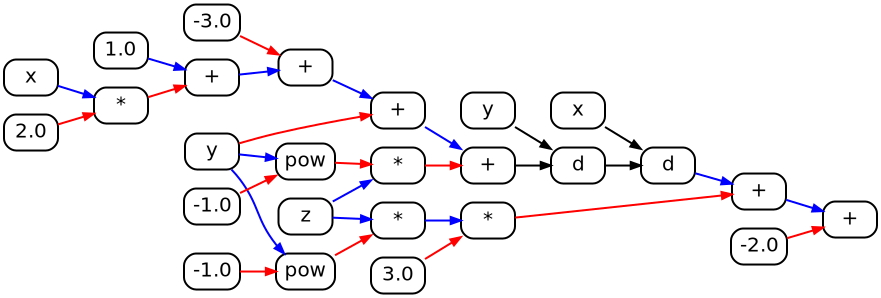
\includegraphics[scale=0.60]{../figures/dataflow.png}
    \input{dfg}
    \caption{Implicit DFG constructed by the original expression, shown above.}
    \label{lst:edsl}
\end{figure}\\\\

\section{Type systems}\label{sec:type-systems}

Early work in type-safe dimension analysis can be found in \citet{kennedy1994dimension, kennedy1996programming} which uses types to encode dimensionality and prevent common bugs related to dimension mismatch from arising, and was later realized in the F\# language~\citep{kennedy2010types}. \citet{jay1996shape}, \citet{rittri1995dimension}, and \citet{zenger1997indexed} explore the application of dimension types for linear algebra. More recently, \citet{kiselyov2005number, kiselyov2010fun} and \citet{griffioen2015type}, show how to manipulate arrays in more complex ways. With the resurgence of interest in tensor algebra and array programming, \citet{chen2017typesafe} and \citet{rink2018modeling} demonstrate how to encode shape-safety for tensor algebra in various type systems.

The problem we attempt to solve can be summarized as follows. Given two values \inline{x} and \inline{y}, and operator \inline{\$}, how do we determine whether the expression \inline{z = x \$ y} is valid, and if so, what is the result type of \inline{z}? For matrix multiplication, when \inline{x} $\in \mathbb{R}^{m \times n}$ and \inline{y} $\in \mathbb{R}^{n \times p}$, the expression is well-typed and we can infer \inline{z} $\in \mathbb{R}^{m \times p}$. More generally, we would like to infer the type of \inline{z} for some operator \inline{@} $: (\mathbb{R}^\mathbf{a}, \mathbb{R}^\mathbf{b}) \rightarrow \mathbb{R}^\mathbf{c}$ where $\mathbf{a} \in \mathbb{N}^q, \mathbf{b} \in \mathbb{N}^r, \mathbf{c} \in \mathbb{N}^s$ and $q, r, s \in \mathbb{N}$. For many linear algebra operations such as matrix multiplication, $\mathcal{T}(\mathbf a, \mathbf b) \stackrel{?}{=} \mathbf c$ is computable in $\mathcal{O}(1)$ -- we can simply check the inner dimensions for equivalence ($\mathbf{a}_2 \stackrel{?}{=} \mathbf{b}_1$).

Shape checking operations on multidimensional arrays is not always decidable. For arbitrary type functions $\mathcal{T}(\mathbf{a}, \mathbf{b})$, checking $\mathcal{T}(\mathbf{a}, \mathbf{b}) \stackrel{?}{=} \mathbf{c}$ requires a Turing machine. If $\mathcal{T}$ is allowed to use the multiplication operator, as in the case of convolutional arithmetic~\citep{dumoulin2016guide}, shape inference becomes equivalent to Peano arithmetic, which is undecidable~\citep{godel1931formal}. Addition, subtraction, indexing and comparison of integers are all decidable operations in Presburger arithmetic~\citep{suzuki1980verification, bradley2006decidable, charlier2011enumeration}. Equality checking is trivially decidable, and can be implemented in most static type systems.

Evaluating an arbitrary $\mathcal{T}$ which uses multiplication or division (e.g.\ convolutional arithmetic) requires a dependently typed language~\citep{xi1998eliminating, pineyro2019structure}, but checking shape equality (e.g. shape checking ordinary arithmetic operations) is feasible in Java and its cousins.\hspace{-.08em}\footnote{Java's type system is known to be Turing complete~\citep{grigore2017java}. Thus, emulation of dependent types in Java is theoretically possible, but likely intractable due to the practical limitations noted by Grigore.} Furthermore, we believe that shape checking ordinary matrix arithmetic is decidable in any type system loosely based on System F${}_{<:}$~\citep{cardelli1991extension}. We propose a type system for enforcing shape-safety which can be implemented in any language with subtyping and generics, such as \href{https://docs.oracle.com/javase/tutorial/java/generics/index.html}{Java}~\citep{naftalin2007java}, \href{https://kotlinlang.org/docs/reference/generics.html}{Kotlin}~\citep{tate2013mixed}, \href{https://www.typescriptlang.org/docs/handbook/advanced-types.html}{TypeScript}~\citep{bierman2014understanding} or \href{https://doc.rust-lang.org/1.7.0/book/generics.html}{Rust}~\citep{crozet2019nalgebra}.

{\tiny
    \begin{table}
        \begin{tabular}{|c|c|c|c|l|}
            \hline
            \multicolumn{1}{|c|}{Math}                             &  Infix                                                                           & Prefix                                                                                    & Postfix                                                                                      & Operator Type Signature                                                                                                                                                                                      \\ \hline
            $A(B)$                                        & \tinline{a(b)}                                                                   &                                                                                           &                                                                                              & $ (\texttt{a}:  \mathbb{R}^{\tau}\rightarrow\mathbb{R}^{\pi}, \texttt{b}: \mathbb{R}^{\lambda} \rightarrow \mathbb{R}^{\tau}) \rightarrow (\mathbb{R}^{\lambda}\rightarrow \mathbb{R}^{\pi})               $ \\ \hline
            $A\pm B$                                      & \begin{tabular}{@{}c@{}}\tinline{a + b}\\\tinline{a - b}\end{tabular}            & \begin{tabular}{@{}c@{}}\tinline{plus(a, b)}\\\tinline{minus(a, b)}\end{tabular}          &                                                                                              & $ (\texttt{a}:  \mathbb{R}^{\tau}\rightarrow\mathbb{R}^{\pi}, \texttt{b}: \mathbb{R}^{\lambda} \rightarrow \mathbb{R}^{\pi}) \rightarrow (\mathbb{R}^{?}\rightarrow \mathbb{R}^{\pi})                      $ \\ \hline
            $A   B$                                       & \begin{tabular}{@{}c@{}}\tinline{a * b}\\\tinline{a.times(b)}\end{tabular}       & \tinline{times(a, b)}                                                                     &                                                                                              & $ (\texttt{a}: \mathbb{R}^{\tau}\rightarrow\mathbb{R}^{m \times n}, \texttt{b}: \mathbb{R}^{\lambda}\rightarrow\mathbb{R}^{n \times p})    \rightarrow (\mathbb{R}^{?}\rightarrow\mathbb{R}^{m \times p})  $ \\ \hline
            \begin{tabular}{@{}c@{}}$\frac{A}{B}$\\$AB^{-1}$\end{tabular}  & \begin{tabular}{@{}c@{}}\tinline{a / b}\\\tinline{a.div(b)}\end{tabular}         & \tinline{div(a, b)}                                                                       &                                                                                              & $ (\texttt{a}: \mathbb{R}^{\tau}\rightarrow\mathbb{R}^{m \times n}, \texttt{b}: \mathbb{R}^{\lambda}\rightarrow\mathbb{R}^{p \times n}) \rightarrow (\mathbb{R}^{?}\rightarrow\mathbb{R}^{m \times p})     $ \\ \hline
            \begin{tabular}{@{}c@{}}$-A$\\$+A$\end{tabular}                &                                                                                  & \begin{tabular}{@{}c@{}}\tinline{-a}\\\tinline{+a}\end{tabular}                           & \begin{tabular}{@{}c@{}}\tinline{a.unaryMinus()}\\\tinline{a.unaryPlus()}\end{tabular}       & $                   (\texttt{a}: \mathbb{R}^{\tau}\rightarrow\mathbb{R}^{\pi}) \rightarrow (\mathbb{R}^{\tau}\rightarrow\mathbb{R}^{\pi})                                                                  $ \\ \hline
%\begin{tabular}{@{}c@{}}sin(a)\\cos(a)\\tan(a)\end{tabular}    &                                                                                  & \begin{tabular}{@{}c@{}}\tinline{sin(a)}\\\tinline{cos(a)}\\\tinline{tan(a)}\end{tabular} & \begin{tabular}{@{}c@{}}\tinline{a.sin()}\\\tinline{a.cos()}\\\tinline{a.tan()}\end{tabular} & $                                            (\texttt{a}: \mathbb{R}\rightarrow\mathbb{R}) \rightarrow (\mathbb{R}\rightarrow\mathbb{R})                                                                   $ \\ \hline
            $\ln(A)$                                       &                                                                                  & \begin{tabular}{@{}c@{}}\tinline{ln(a)}\\\tinline{log(a)}\end{tabular}                    & \begin{tabular}{@{}c@{}}\tinline{a.ln()}\\\tinline{a.log()}\end{tabular}                     & $                  (\texttt{a}: \mathbb{R}^{\tau}\rightarrow\mathbb{R}^{m \times m}) \rightarrow (\mathbb{R}^{\tau}\rightarrow\mathbb{R}^{m \times m})                                                     $ \\ \hline
            $\log_b A$                                      & \tinline{a.log(b)}                                                               & \tinline{log(a, b)}                                                                       &                                                                                              & $       (\texttt{a}: \mathbb{R}^{\tau}\rightarrow\mathbb{R}^{m \times m}, \texttt{b}: \mathbb{R}^{\lambda}\rightarrow\mathbb{R}^{m \times m}) \rightarrow (\mathbb{R}^{?}\rightarrow\mathbb{R})            $ \\ \hline
            $A^{b}$                                        & \tinline{a.pow(b)}                                                               & \tinline{pow(a, b)}                                                                       &                                                                                              & $       (\texttt{a}: \mathbb{R}^{\tau}\rightarrow\mathbb{R}^{m \times m}, \texttt{b}: \mathbb{R}^{\lambda}\rightarrow\mathbb{R}) \rightarrow (\mathbb{R}^{?}\rightarrow\mathbb{R}^{m \times m})            $ \\ \hline
            \begin{tabular}{@{}c@{}}$\sqrt{a}$\\$\sqrt[3]{a}$\end{tabular} & \begin{tabular}{@{}c@{}}\tinline{a.pow(1.0/2)}\\\tinline{a.root(3)}\end{tabular} & \begin{tabular}{@{}c@{}}\tinline{a.pow(1.0/2)}\\\tinline{a.root(3)}\end{tabular}          & \begin{tabular}{@{}c@{}}\tinline{a.sqrt()}\\\tinline{a.cbrt()}\end{tabular}                  & $                        (\texttt{a}: \mathbb{R}^{\tau}\rightarrow\mathbb{R}^{m \times m}) \rightarrow (\mathbb{R}\rightarrow\mathbb{R}^{m \times m})                                                      $ \\ \hline
            \begin{tabular}{@{}c@{}}$\frac{da}{db}$\\$a'(b)$\end{tabular}  & \tinline{a.d(b)}                                                                 & \tinline{grad(a)[b]}                                                                      & \tinline{d(a) / d(b)}                                                                        & $         (\texttt{a}: \mathbb{R}^{\tau}\rightarrow\mathbb{R}^{\pi}, \texttt{b}: \mathbb{R}^{\lambda}\rightarrow\mathbb{R}^{\omega}) \rightarrow (\mathbb{R}^{?}\rightarrow\mathbb{R}^{\pi \times \omega}) $ \\ \hline
        \end{tabular}
        \caption{\label{tab:shape_system}Kotlin$\nabla$'s shape system specifies the output shape for tensor expressions.}
    \end{table}
}
%$\dagger$ \inline{a} and \inline{b} are higher order functions. These may be constants (e.g. 0, 1.0), variables (e.g. \inline{Var("x")}) or expressions (e.g. \inline{x + 1}, \inline{2 * x + y}).

\section{Shape safety}\label{sec:shape-safety}

\noindent There are three broad strategies for handling shape errors in array programming: \\
%
\begin{enumerate}
    \item Conceal the error by implicitly reshaping or \href{https://docs.scipy.org/doc/numpy-1.15.0/user/basics.broadcasting.html}{broadcasting arrays}.
    \item Announce the error at runtime with a relevant message, e.g.~\href{https://www.tensorflow.org/api_docs/python/tf/errors/InvalidArgumentError}{\inline{InvalidArgumentError}}.
    \item Do not allow programs which can result in a shape error to compile. \\
\end{enumerate}
%
Most array programming libraries such as NumPy~\citep{van2011numpy} or TensorFlow~\citep{abadi2016tensorflow} use the first or second strategy. In Kotlin$\nabla$, we adopt the third, which allows an incremental type checker, such as those typically found in modern IDEs, to instantaneously detect when a matrix operation is invalid. Consider the following example:
%
\begin{kotlinlisting}
val vecA = Vec(1.0, 2.0)      // Inferred type: Vec<Int, D2>
val vecB = Vec(1.0, 2.0, 3.0) // Inferred type: Vec<Int, D3>
val vecC = vecB + vecB
val vecD = (*\uwave{vecA + vecB}*) // Compile error: Expected Vec<2>, found Vec<3>
\end{kotlinlisting}
%
Attempting to sum two vectors whose shapes do not match will fail to compile.
%
\begin{kotlinlisting}
val matA = Mat1x4(1.0, 2.0, 3.0, 4.0) // Inferred type: Mat<Double, D1, D4>
val matB = Mat4x1(1.0, 2.0, 3.0, 4.0) // Inferred type: Mat<Double, D4, D1>
val matC = matA * matB
val matD = (*\uwave{matA *\ matC}*) // Compile error: Expected Mat<4, *>, found Mat<1, 1>
\end{kotlinlisting}
%
Similarly, multiplying two matrices whose inner dimensions do not match will not compile.
%
\begin{kotlinlisting}
val matA = Mat2x4(1.0, 2.0, 3.0, 4.0,
                  5.0, 6.0, 7.0, 8.0)
val matB = Mat4x2(1.0, 2.0,
                  3.0, 4.0,
                  5.0, 6.0,
                  7.0, 8.0)
val matC: Mat<Double, D2, D2> = a * b // Types are optional, but encouraged
val matD = Mat2x1(1.0, 2.0)
val matE = matC * matD
val matF = Mat3x1(1.0, 2.0, 3.0)
val matG = (*\uwave{matE *\ matF}*) // Compile error: Expected Mat<1, *>, found Mat<3, 1>
\end{kotlinlisting}
%
It is required to specify the parameter types in a method signature. Explicit return types are optional but encouraged for readability. If omitted, the type system can often infer them:
%
\begin{kotlinlisting}
fun someMatFun(m: Mat<Double, D3, D1>): Mat<Double, D3, D3> = ...
fun someMatFun(m: Mat<Double, D2, D2>) = ...
\end{kotlinlisting}
%
Shape safety is currently supported up to rank-2 tensors, i.e.\ matrices. To perform dimension checking in our type system, first we enumerate a list of integer type literals as a chain of subtypes, $C <: C - 1 <: C - 2 <: \dots <: 1 <: 0$, where $C$ is the largest fixed-length dimension we wish to represent, which can be specified by the user prior to compilation. This guarantees linear space and time complexity for subtype checking, with a constant upper bound.
%
\begin{kotlinlisting}[caption={Shape safe tensor addition for rank-1 tensors, $\forall C\leq2.$}]
interface Nat<T: D0> { val i: Int }
// Integer literals have reified Int values should we need to compare them at runtime
sealed class D0(open val i: Int = 0) { companion object: D0(), Nat<D0> }
sealed class D1(override val i: Int = 1): D0(i) { companion object: D1(), Nat<D1> }
sealed class D2(override val i: Int = 2): D1(i) { companion object: D2(), Nat<D2> }
sealed class D3(override val i: Int = 3): D2(i) { companion object: D3(), Nat<D3> }
//...Code for integer literals should be generated
sealed class D99(override val i: Int = 99): D98(i) { companion object: D99(), Nat<D99> }
\end{kotlinlisting}
%
Next, we overload the call operator to emulate instantiating a collection literal, using arity to infer its dimensionality. Consider the rank-1 case for length inference on vector literals:
%
\begin{kotlinlisting}
open class Vec<E, Len: D1> constructor(val contents: List<E>) {
    companion object {
        operator fun <T> invoke(t: T): Vec<T, D1> = Vec(listOf(t))
        operator fun <T> invoke(t0: T, t1: T): Vec<T, D2> = Vec(listOf(t0, t1))
        operator fun <T> invoke(t0: T, t1: T, t2: T): Vec<T, D3> = Vec(listOf(t0, t1, t2))
    }
}
\end{kotlinlisting}
%
Finally, we overload arithmetical operators using generic shape constraints. Since our type-level integers are a chain of subtypes, we only need to define one operator and can rely on Liskov substitution~\citep{liskov1987} to preserve shape safety for all subtypes.
%
\begin{kotlinlisting}
// <C: D1> will accept 1 <= C <= 99 via Liskov substitution
operator fun <E, C: D1, V: Vec<X, C>> V.plus(v: V): V = TODO()
\end{kotlinlisting}
%
The operator \inline{+} can now be used like so. Incompatible operands will cause a type error:
%
\begin{kotlinlisting}
// Type-checked vector addition with shape inference
val Y = Vec(0, 0) + Vec(0, 0) // Y: Vec<Float, D2>
val X = (*\uwave{Vec(0, 0) + Vec(0, 0, 0)}*) // Compile error: Expected Vec<Int, D2>, found Vec<Int, D3>
\end{kotlinlisting}
%
Dynamic length construction is also permitted, although it may fail at runtime. For example:
%
\begin{kotlinlisting}
val one = Vec(0, 0, 0) + Vec(0, 0, 0) // Always runs safely
val add = Vec(0, 0, 0) + Vec<Int, D3>(listOf(...)) // Compiles, but may fail at runtime
val vec = Vec(0, 0, 0) // Inferred type: Vec<3>
val sum = (*\uwave{Vec(0, 0) + add}*) // Compile error: Expected Vec<Int, D2>, found Vec<Int, D3>
\end{kotlinlisting}
%
Matrices and tensors have a similar syntax. For example, Kotlin$\nabla$ can infer the shape of matrix multiplication, and will not compile if the arguments' inner dimensions disagree:
%
\begin{kotlinlisting}
open class Mat<X, R: D1, C: D1>(vararg val rows: Vec<X, C>)
fun <X> Mat1x2(d0: X, d1: X): Mat<X, D1, D2> = Mat(Vec(d0, d1))
fun <X> Mat2x1(d0: X, d1: X): Mat<X, D2, D1> = Mat(Vec(d0), Vec(d1))

operator fun <X, Q: D1, R: D1, S: D1> Mat<X, Q, R>.times(m: Mat<X, R, S>): Mat<X, Q, S> =
    Mt( *(rows.indices).map { i -> /* ... */ }.toTypedArray() )

val matM = Mat1x2(0, 0)
val matO = (*\uwave{matM *\ matM}*) // Compile error: Expected Mat<2, *>, found Mat<1, 2>
\end{kotlinlisting}
%
A similar technique can be found in nalgebra~\citep{crozet2019nalgebra}, a shape-checked linear algebra library for the Rust language which also uses synthetic type-level integers. This technique originates in Haskell, a language which supports more powerful forms of type-level computation, such as \textit{type arithmetic}~\citep{kiselyov2005number}. Type arithmetic simplifies array concatenation, convolutional arithmetic~\citep{dumoulin2016guide} and other operations which are currently difficult to express in Kotlin$\nabla$, where arbitrary type-level functions $\mathcal{T}(\mathbf a, \mathbf b)$ (ref.~\autoref{sec:type-systems}) can require enumerating up to $C^{q + r}$ Kotlin functions to compute.

\section{Testing}\label{sec:testing}

Kotlin$\nabla$ claims to eliminate certain runtime errors, but how do we know the implementation is not incorrect? One method is known as property-based testing (PBT)~\citep{fink1997property} (\autoref{subsec:property-based-testing}), closely related to the notion of metamorphic testing~\citep{chen1998metamorphic} (\autoref{subsec:metamorphic-testing}). Notable implementations include \href{http://www.cse.chalmers.se/~rjmh/QuickCheck/manual.html}{QuickCheck}~\citep{claessen2011quickcheck}, \href{https://hypothesis.readthedocs.io/en/latest/}{Hypothesis}~\citep{Hypothesis} and \href{https://github.com/kotlintest/kotlintest}{KotlinTest}~\citep{kotlintest}, on which our test suite is based. PBT uses algebraic properties to verify the result of a calculation by constructing semantically equivalent but syntactically distinct expressions. When evaluated on the same inputs, these should produce the same answer, to within numerical precision. Two such equivalences are used to test Kotlin$\nabla$: \\
%
\begin{enumerate}
    \item \textbf{Analytical differentiation}: manually differentiate selected functions and compare the numerical result of evaluating random chosen inputs from their domain with the numerical result obtained by evaluating AD on the same inputs.
    \item \textbf{Finite difference approximation}: sample the space of symbolic differentiable functions, comparing the numerical results suggested by the \hyperref[sec:fdm]{finite difference method} and the equivalent AD result, up to a fixed-precision approximation. \\
\end{enumerate}
%
For example, the following test checks whether the analytical derivative and the automatic derivative, when evaluated at random points, are equal to within numerical precision:
%
\begin{kotlinlisting}
val x = Var("x")
val y = Var("y")
val z = y * (sin(x * y) - x)            // Function under test
val dz_dx = d(z) / d(x)                 // Automatic derivative
val manualDx = y * (cos(x * y) * y - 1) // Manual derivative

"dz/dx should be y * (cos(x * y) * y - 1)" {
    NumericalGenerator.assertAll { x0, y0 ->
    // Evaluate the results at a given seed
    val autoEval = dz_dx(x to x0, y to y0)
        val manualEval = manualDx(x to x0, y to y0)
        autoEval shouldBeApproximately manualEval // Fails iff eps < |adEval - manualEval|
    }
}
\end{kotlinlisting}
%
PBT will search the input space for two numerical values \inline{x0} and \inline{y0}, which violate the specification, then ``shrink'' them to discover pass-fail boundary values. We can construct a similar test using the \hyperref[sec:fdm]{finite difference method}, e.g. $f'(x)=\lim _{h\to 0}{\frac {f(x+h)-f(x)}{h}}$:
%
\begin{kotlinlisting}
val dx = 1E-8
val x = Var("x")
val f = sin(x)
val df_dx = d(f) / d(x)
val fd_dx = (sin(x + dx) - sin(x)) / dx

"d(sin x)/dx should be equal to (sin(x + dx) - sin(x)) / dx" {
    NumericalGenerator.assertAll { x0 ->
    val autoEval = df_dx(x0)
        val fdEval = fd_dx(x0)
        autoEval shouldBeApproximately fdEval // Fails iff eps < |adEval - fdEval|
    }
}
\end{kotlinlisting}
%
There are many other ways to independently verify the numerical gradient, such as dual numbers or the complex step derivative. Another method to validate Kotlin$\nabla$'s implementation would be to compare the numerical output against the output of a well-known AD framework, such as TensorFlow. In future work, we intend to conduct a more thorough comparison of numerical accuracy and performance.

\section{Operator overloading}\label{sec:operator-overloading}

\noindent Operator overloading~\citep{corliss1993operator} is one of the simplest ways to implement automatic differentiation. We use Kotlin's \href{https://kotlinlang.org/docs/reference/operator-overloading.html}{operator overloading} functionality on a numeric tower (ref. ~\autoref{sec:numeric-tower}) to provide a concise notation for abstract algebraic operations. For example, suppose we have an interface \inline{Group}, which overloads the operators \inline{+} and \inline{*}:
%
\begin{kotlinlisting}
interface Group<T: Group<T>> {
    operator fun plus(addend: T): T
    operator fun times(multiplicand: T): T
}
\end{kotlinlisting}
%
Here, we specify a recursive type bound using a method known as F-bounded polymorphism~\citep{canning1989f} to ensure that operations return the concrete value of the type variable \inline{T}, rather than something more abstract like \inline{Group} (effectively, \inline{T} is a \inline{self} type). Imagine a class \inline{Fun} which has implemented \inline{Group}. It can be used as follows:
%
\begin{kotlinlisting}
fun <T: Group<T>> cubed(t: T): T = t * t * t
fun <X: Fun<X>> twiceExprCubed(e: X): X = cubed(e) + cubed(e)
\end{kotlinlisting}
%
Like \href{https://docs.python.org/3/reference/datamodel.html#special-method-names}{Python}, Kotlin supports overloading a limited set of operators, which are evaluated using a \href{https://kotlinlang.org/docs/reference/grammar.html#precedence}{fixed precedence}. In the current version of Kotlin$\nabla$, operators do not perform any computation, they simply construct a directed acyclic graph representing the symbolic expression. Expressions are only evaluated when invoked as a function.

\section{First-class functions}\label{sec:first-class-functions}

By supporting higher-order functions and lambdas, Kotlin treats functions as first-class citizens. This allows us to represent mathematical functions and programming functions with the same underlying abstractions (i.e.\ typed FP). Following a number of recent papers in functional AD~\citep{pearlmutter2008reverse,wang2018backpropagation}, all expressions in Kotlin$\nabla$ are treated as functions. For example:

\begin{kotlinlisting}
fun <T: Group<T>> makePoly(x: Var<T>, y: Var<T>) = x * y + y * y + x * x
val x: Var<DoubleReal> = Var()
val y: Var<DoubleReal> = Var()
val f = makePoly(x, y)
val z = f(1.0, 2.0) // Returns a value
println(z) // Prints: 7
\end{kotlinlisting}
%
Currently, it is possible to represent functions where all inputs and outputs share a single data type. It may be possible to extend support for building functions with varying input/output types and enforcing constraints on both, by using covariant and contravariant type bounds.

\section{Numeric Tower}\label{sec:numeric-tower}

Kotlin$\nabla$ uses a numeric tower~\citep{st2012typing}. An early example of this pattern can be found in \href{https://www.gnu.org/software/guile/manual/html_node/Numerical-Tower.html}{Scheme}~\citep{sperber2009revised}. This strategy is also suited to object oriented languages~\citep{niculescu2003design, niculescu2011using, kennedy2005generalized} and applied in libraries such as \href{https://github.com/mipt-npm/kmath}{KMath}~\citep{nozik2019kmath} and \href{https://commons.apache.org/proper/commons-math/}{Apache Commons Math}~\citep{developers2012apache}.

\begin{kotlinlisting}
interface Group<X: Group<X>> {
    operator fun unaryMinus(): X
    operator fun plus(addend: X): X
    operator fun minus(subtrahend: X): X = this + -subtrahend
    operator fun times(multiplicand: X): X
}

interface Field<X: Field<X>> : Group<X> {
    val e: X
    val one: X
    val zero: X
    operator fun div(divisor: X): X = this * divisor.pow(-one)
    infix fun pow(exp: X): X
    fun ln(): X
}
\end{kotlinlisting}
%
The numeric tower allows us to define common behavior such as subtraction and division on abstract algebraic structures, e.g. \inline{Group}, \inline{Ring}, and \inline{Field}. These abstractions are extensible to concrete number systems, such as complex numbers and quaternions. For example, to later define a field over complex numbers or quaternions,\hspace{-.08em}\footnote{ex. In order to calculate derivatives in a quaternion neural network. \citep{isokawa2003quaternion}} one must simply extend the numeric tower and override the default implementation. Most mathematical operations can be defined using a small set of primitive operators, which can be differentiated in a generic fashion, rather than on an ad hoc basis.

\section{Algebraic data types}\label{sec:adts}

\noindent Algebraic data types (ADTs) in the form of \href{https://kotlinlang.org/docs/reference/sealed-classes.html}{sealed classes} (a.k.a.\ sum types) facilitate a limited form of pattern matching over a closed set of subclasses. When matching against subclasses of a sealed class, the compiler forces the author to provide an exhaustive control flow over all concrete subtypes of an abstract class. Consider the following classes:
%
\begin{kotlinlisting}
class Const<T: Fun<T>>(val number: Number) : Fun<T>()
class Sum<T: Fun<T>>(val left: Fun<T>, val right: Fun<T>) : Fun<T>()
class Prod<T: Fun<T>>(val left: Fun<T>, val right: Fun<T>) : Fun<T>()
class Var<T: Fun<T>> : Fun<T>() { override val variables: Set<Var<X>> = setOf(this) }
class Zero<T: Fun<T>> : Const<T>(0.0)
class One<T: Fun<T>> : Const<T>(1.0)
\end{kotlinlisting}
%
When branching on the type of a sealed class, consumers must explicitly handle every case, since incomplete control flow will not compile rather than fail silently at runtime. Let us now consider a simplified definition of \inline{Fun}, a sealed class which defines the behavior of function invocation and differentiation, using a restricted form of pattern matching. It can be constructed with a set of \inline{Var}s, and can be invoked with a numerical value:
%
\begin{kotlinlisting}
sealed class Fun<X: Fun<X>>(open val variables: Set<Var<X>> = emptySet()) : Group<Fun<X>> {
    constructor(vararg fns: Fun<X>): this(fns.flatMap { it.variables }.toSet())
    // Since the subclasses of Fun are a closed set, no `else -> ...` is required.
    operator fun invoke(map: Map<Var<X>, X>): Fun<X> = when (this) {
        is Const -> this
        is Var -> map.getOrElse(this) { this } // Partial application is permitted
        is Prod -> left(map) * right(map) // Smart casting implicitly casts after checking
        is Sum -> left(map) + right(map)
    }

    fun d(variable: Var<X>): Fun<X> = when(this) {
        is Const -> Zero
        is Var -> if (variable == this) One else Zero
        // Product rule: d(u*v)/dx = du/dx * v + u * dv/dx
        is Prod -> left.d(variable) * right + left * right.d(variable)
        is Sum -> left.d(variable) + right.d(variable)
    }

    operator fun plus(addend: Fun<T>) = Sum(this, addend)
    operator fun times(multiplicand: Fun<T>) = Prod(this, multiplicand)
}
\end{kotlinlisting}
%
Kotlin's \href{https://kotlinlang.org/docs/reference/typecasts.html#smart-casts}{smart casting} is an example of flow-sensitive type analysis~\citep{pearce2011implementing} where the abstract type \inline{Fun} can be treated as \inline{Sum} after performing an \inline{is Sum} check. Without smart casting, we would need to write \inline{(this as Sum).left} to access the member, \inline{left}, creating a potential \inline{ClassCastException} if the cast were mistaken.

\section{Multiple Dispatch}\label{sec:multiple-dispatch}

In conjunction with ADTs, Kotlin$\nabla$ uses multiple dispatch to instantiate the most specific result type of an arithmetic operation based on the type of its operands. Although Kotlin does not directly support multiple dispatch, it can be emulated using single dispatch as described by \citet{leavens1998multiple}. Building on \autoref{sec:adts}, suppose we wish to rewrite some algebraic expression, e.g. to reduce expression swell or improve numerical stability. We can use \inline{when} to branch on the type of a subexpression at runtime:

\begin{kotlinlisting}
override fun times(multiplicand: Fun<X>): Fun<X> =
    when {
        this == zero -> this
        this == one -> multiplicand
        multiplicand == one -> this
        multiplicand == zero -> multiplicand
        this == multiplicand -> pow(two)
        // w/o smart cast: Const((this as Const).number * (multiplicand as Const).number)
        this is Const && multiplicand is Const -> Const(number * multiplicand.number)
        // Further simplification is possible using rules of replacement
        else -> Prod(this, multiplicand)
    }

val result = Const(2.0) * Sum(Var(2.0), Const(3.0))
//         = Sum(Prod(Const(2.0), Var(2.0)), Const(6.0))
\end{kotlinlisting}
%
Multiple dispatch allows us to put all related control flow on a single abstract class which is inherited by subclasses, simplifying readability, debugging and refactoring.

\section{Extension Functions}\label{sec:extension-functions}

\href{https://kotlinlang.org/docs/reference/extensions.html}{Extension functions} augment external classes with new fields and methods. By using context-oriented programming~\citep{hirschfeld2008context}, we can expose custom extensions (e.g.\ through \inline{DoubleContext}) to consumers without requiring subclassing or inheritance.
%
\begin{kotlinlisting}[caption={We can provide numerical extensions, wrapped in a context.}]
object DoubleContext {
    operator fun Number.times(expr: Fun<Double>) = Const(toDouble()) * expr
}
\end{kotlinlisting}
%
Now, we can use the context to define another extension, \inline{Fun.multiplyByTwo()}, which computes the product inside a \inline{DoubleContext}, using the operator overload defined above:
%
\begin{kotlinlisting}
fun Fun<Double>.multiplyByTwo() = with(DoubleContext) { 2 * this }
\end{kotlinlisting}
%
Extensions can also be defined in another file or context and imported on demand, an approach borrowed from \href{https://github.com/mipt-npm/kmath}{KMath}~\citep{nozik2019kmath}, another mathematical library for Kotlin. This approach is also suitable for defining convenience methods for variable assignment and type adapters for numerical primitives in a context sensitive manner. For example:
%
\begin{kotlinlisting}
object DoubleContext: Proto<DConst, Double>() {
    override val Const<DConst, Number>.value: Double
    get() = c.toDouble()
    override fun wrap(default: Number): DConst = DConst(default.toDouble())
    override val X: X<DConst> = object: X<DConst>(DConst(0.0)) {
        override fun invoke(X: XBnd<DConst>): DConst = X.const
        override fun toString() = "X"
    }
    override val Y: Y<DConst> = object: Y<DConst>(DConst(0.0)) {
        override fun invoke(Y: YBnd<DConst>): DConst = Y.const
        override fun toString() = "Y"
    }
    override infix fun X<DConst>.to(c: Double) = XBnd(DConst(c))
    override infix fun Y<DConst>.to(c: Double) = YBnd(DConst(c))
}
\end{kotlinlisting}
%
This DSL, which is used to support variable capture and currying, can be used as follows:
%
\begin{kotlinlisting}
with(DoubleContext) {
    val t = X + Y + 0.0
    val l = t(X to 1.0, Y to 2.0)
    val r = t(X to 1.0)(Y to 3.0) // Currying
    val o = X + Z + 0.0
    val p = o(X to 1.0) // Partial application
    val k = (*\uwave{o(Y to 4.0)}*) // Does not compile
}
\end{kotlinlisting}

\section{Automatic, Symbolic Differentiation}

It has long been claimed by the AD literature that automatic differentiation is not symbolic differentiation~\citep{baydin2015survey}. Many, including the author of this thesis, have suspected this claim to be misleading. Recently, the claim has been questioned~\citep{wang2018demystifying} and refuted~\citep{laue2019equivalence}. While it may be true that certain implementations of automatic differentiation interleave numerical evaluation and symbolic differentiation at runtime, this interleaving is certainly not a prerequisite for a differentiation library to be considered \textit{automatic}. Nor, as suggested by prior literature~\citep{baydin2014ad}, is the problem of expression swell unique to symbolic differentiation~\citep{laue2019equivalence}, whose findings we can numerically reproduce as shown in ~\autoref{fig:pbt_comparison}.

The distinction between AD and SD becomes increasingly blurry when we consider more flexible execution models~\citep{wang2018demystifying} and hybrid ADs~\citep{abadi2016tensorflow} which are capable of both eager~\citep{agrawal2019tensorflow} and lazy evaluation. Instead, we take the view that symbolic differentiation is a type of automatic differentiation which the AD literature has been too quick to dismiss. SD in particular, affords the compiler far more flexibility to perform global optimizations such as algebraic simplification~\citep{bergstra2010theano}, loop vectorization~\citep{agarwal2019static} and tensor comprehension~\citep{vasilache2018tensor}. These optimizations would otherwise be impossible if their symbolic differentiation and numerical evaluation were performed in lockstep, when the dataflow graph is only partially available.

\section{Coroutines}\label{sec:coroutines}

Coroutines are a generalization of subroutines for non-preemptive multitasking, typically implemented using continuations~\citep{haynes1984continuations}. Continuations are a mechanism that allow functions to access and modify subsequent computation. In continuation-passing style~\citep{sussman1975scheme} (CPS), every function, in addition to its usual arguments, takes another function representing the subsequent routine. Rather than returning to its caller after completion, the function invokes its continuation, and the process is restarted.

One form of continuation, known as delimited continuations, are sufficient for implementing reverse-mode AD with operator overloading alone (without any additional data structures) as described by \citet{wang2018demystifying} and later in \citet{wang2018backpropagation}. Delimited continuations can be implemented with \href{https://kotlinlang.org/docs/reference/coroutines-overview.html}{Kotlin Coroutines}, and merits further investigation.

\section{Comparison}\label{sec:comparison}

Inspired by \href{https://github.com/Functional-AutoDiff/STALINGRAD}{Stalin$\nabla$}~\citep{pearlmutter2008using}, \href{https://github.com/HIPS/autograd/}{Autograd}~\citep{maclaurin2015autograd, maclaurin2016phd}, \href{http://deeplearning.net/software/theano/}{Theano}~\citep{bergstra2010theano}, \href{https://github.com/mila-iqia/myia}{Myia}~\citep{breuleux2017automatic, vanmerrienboer2018ad}, \href{https://github.com/uniker9/JAutoDiff/}{JAutoDiff}~\citep{nureki2012jautodiff}, \href{https://tongfei.me/nexus/}{Nexus}~\citep{chen2017typesafe}, \href{https://feiwang3311.github.io/Lantern/}{Lantern}~\citep{wang2018demystifying}, \href{https://github.com/google/tangent}{Tangent}~\citep{van2018tangent}, \citet{elliott2018simple}, \href{https://people.csail.mit.edu/tzumao/gradient_halide/}{Halide}~\citep{li2018halide} et al., Kotlin$\nabla$ attempts to port recent developments in automatic differentiation (AD) to the Kotlin language. In the process, it introduces a number of experimental ideas, including \hyperref[sec:shape-safety]{compile-time shape-safety}, \hyperref[sec:multiple-dispatch]{algebraic simplification} and numerical stability checking through \hyperref[sec:testing]{property-based testing}. Prior work, including \href{https://pytorch.org/}{PyTorch}~\citep{paszke2017automatic}, \href{https://www.tensorflow.org/}{TensorFlow}~\citep{abadi2016tensorflow}, \href{https://chainer.org/}{Chainer}~\citep{chainer}, \href{https://deeplearning4j.org/}{DL4J}~\cite{team2016dl4j} and others have developed general-purpose AD libraries in less safe languages.

Unlike most existing AD implementations, Kotlin$\nabla$ is a purely symbolic, graph-based AD that does not require any template metaprogramming, compiler augmentation or runtime reflection to ensure type safety. As we have seen, this approach is primarily achieved through \hyperref[sec:operator-overloading]{operator overloading}, parametric polymorphism, and \hyperref[sec:adts]{pattern matching}. The practical advantage of this approach is that it can be implemented as a simple library or embedded domain-specific language (eDSL), thereby leveraging the host language's type system to receive code completion and type inference for free. Our approach is particularly well-suited to functional programming, and employs several functional programming concepts, including lambda expressions, higher order functions, partial application, currying and algebraic data types. For a more detailed comparison of Kotlin$\nabla$ with existing AD libraries, see \autoref{tab:ad_comparison}.\\

\begin{table}
    \begin{tabular}{llllllllll}
        Framework & Language &
        \rot{Symbolic Differentiation} &
        \rot{Automatic Differentiation} &
        \rot{Differentiable Programming} &
        \rot{Functional Programming} &
        \rot{Type-Safe} &
        \rot{Shape-Safe} &
        \rot{Dependently-Typed} &
        \rot{Multiplatform}
        \\ \hline
        \href{https://github.com/breandan/kotlingrad}{Kotlin$\nabla$}                    & Kotlin  & \cmark & \cmark & \wmark & \cmark & \cmark & \cmark & \xmark & \wmark \\
        \href{https://diffsharp.github.io/DiffSharp/}{DiffSharp}                          & F\#     & \xmark & \cmark & \cmark & \cmark & \cmark & \xmark & \xmark & \xmark \\
        \href{https://github.com/fsprojects/fsharp-ai-tools}{TensorFlow.FSharp}          & F\#     & \xmark & \cmark & \cmark & \cmark & \cmark & \cmark & \xmark & \xmark \\
%\href{https://github.com/ThoughtWorksInc/DeepLearning.scala}{DeepLearning.scala} & Scala   & \xmark & \cmark & \cmark & \cmark & \cmark & \xmark & \xmark & \xmark \\
        \href{https://tongfei.me/nexus/}{Nexus}                                          & Scala   & \xmark & \cmark & \cmark & \cmark & \cmark & \cmark & \xmark & \xmark \\
        \href{https://feiwang3311.github.io/Lantern/}{Lantern}                           & Scala   & \xmark & \cmark & \cmark & \cmark & \cmark & \xmark & \xmark & \xmark \\
%\href{https://github.com/HuwCampbell/grenade}{Grenade}                           & Haskell & \xmark & \cmark & \xmark & \cmark & \cmark & \cmark & \xmark & \xmark \\
        \href{https://github.com/leopiney/tensor-safe}{Tensor Safe}                      & Haskell & \xmark & \cmark & \xmark & \cmark & \cmark & \cmark & \cmark & \xmark \\
        \href{https://github.com/hasktorch/hasktorch}{Hasktorch}                         & Haskell & \xmark & \cmark & \cmark & \cmark & \cmark & \cmark & \xmark & \xmark \\
        \href{https://deeplearning4j.org}{Eclipse DL4J}                                  & Java    & \xmark & \cmark & \xmark & \xmark & \cmark & \xmark & \xmark & \xmark \\
        \href{https://uniker9.github.io/JAutoDiff/}{JAutoDiff}                            & Java    & \cmark & \cmark & \xmark & \xmark & \cmark & \xmark & \xmark & \xmark \\
%\href{https://halide-lang.org}{Halide}                                           & C++     & \xmark & \cmark & \cmark & \xmark & \cmark & \xmark & \xmark & \xmark \\
        \href{https://github.com/Functional-AutoDiff/STALINGRAD}{Stalin$\nabla$}         & Scheme  & \xmark & \cmark & \xmark & \xmark & \xmark & \xmark & \xmark & \xmark \\
        \href{https://github.com/mila-iqia/myia}{Myia}                                   & Python  & \cmark & \cmark & \cmark & \cmark & \xmark & \xmark & \xmark & \wmark \\
% \href{https://github.com/HIPS/autograd/}{Autograd}                               & Python  & \xmark & \cmark & \xmark & \xmark & \xmark & \xmark & \xmark & \xmark \\
        \href{https://github.com/google/jax}{JAX}                                        & Python  & \xmark & \cmark & \cmark & \cmark & \xmark & \xmark & \xmark & \wmark \\
        \href{https://github.com/google/tangent}{Tangent}                                & Python  & \xmark & \cmark & \xmark & \xmark & \xmark & \xmark & \xmark & \xmark \\

    \end{tabular}
    \caption{\label{tab:ad_comparison} Comparison of AD libraries. The \wmark symbol indicates work in progress.}
\end{table}

\vspace{-20pt}\section{Future work}\label{sec:future-work}

%\vspace{40pt}\setlength{\epigraphwidth}{0.80\textwidth}
%\epigraph{``It is well known that the central problem of the whole of modern mathematics is the study of the transcendental functions defined by differential equations.''}{\begin{flushright}--Felix \citet{klein1893lectures}, \textit{Lectures on mathematics}\end{flushright}}

\vspace{2pt}\setlength{\epigraphwidth}{0.65\textwidth}
\epigraph{``The derivative, as this notion appears in the elementary differential calculus, is a familiar mathematical example of a function for which both [the domain and the range] consist of functions.''}{\begin{flushright}--Alonzo \citet{church1941calculi}, \href{https://archive.org/details/AnnalsOfMathematicalStudies6ChurchAlonzoTheCalculiOfLambdaConversionPrincetonUniversityPress1941}{\textit{The Calculi of Lambda Conversion}}\end{flushright}}

The derivative, as it is most commonly used, is usually associated with the calculus of infinitesimals. But the same rules for symbolic differentiation introduced by Leibniz and Newton over three centuries ago have reappeared in strange and marvelous places throughout computer science. In \citet{brzozowski1964derivatives}, we encounter an example of symbolic differentiation in a discrete setting, i.e. regular expressions. Brzozowski's work has important and far-reaching applications in automata theory~\citep{berry1986regex, antimirov1996partial, champarnaud1999regular} and incremental parsing~\citep{might2011parsing, moss2014derivatives}. Later in \citet{thayse1981boolean} the boolean differential calculus was first introduced,\hspace{-.08em}\footnote{Although early work on the subject can be traced back to \citet{talantsev1959analysis} and \citet{sellers1968analyzing}} a branch of boolean algebra which has important applications in switching theory~\citep{thayse1973boolean} and synthesis of digital circuits~\citep{steinbach2017boolean}. Symbolic differentiation has useful applications in other mathematical settings, including $\lambda$-calculus~\citep{ehrhard2003differential, cai2014theory, kelly2016evolving, brunel2020backpropagation}, incremental computation~\citep{alvarez2019fixing, alvarez2019change}, type theory~\citep{mcbride2001derivative, mcbride2008clowns, chen2012type}, category theory~\citep{blute2006differential, blute2009cartesian}, domain theory~\citep{edalat2002domain}, probability theory~\citep{kac1951probability} and linear logic~\citep{ehrhard2018introduction, clift2018derivatives}.

Many further examples of symbolic differentiation can be found in unrelated bodies of literature. This pattern seems unlikely to be mere coincidence, and suggests an unrealized connection between differential and algebraic geometry, perhaps holding important insights for differentiable programming and the study of change propagation in computation graphs.

The work described in this chapter establishes a framework for exploring symbolic differentiation using algebraic structures like \inline{Group}, \inline{Ring}, and \inline{Field} (\autoref{sec:numeric-tower}). In future work, we hope to explore the relationship between differentiable programming and symbolic differentiation in other topologies. Perhaps there exists an analogous mechanism to gradient descent which can be exploited to accelerate optimization in such spaces, e.g. for learning boolean variables and other data structures like graphs and trees.

As shown in prior literature~\citep{bergstra2010theano, baydin2015survey, laue2019equivalence}, intermediate expression swell is a pernicious issue in computer algebra and automatic differentiation. The ad-hoc algebraic simplification procedure described in \autoref{sec:multiple-dispatch} is almost certainly inadequate for general use cases. One interesting direction would be training a model to minimize numerical drift, by applying general-purpose rewriting rules. There exists a long list of prior work in rewriting algorithms for numerical stability, dating back to \citet{kahan1965summation, dekker1971floating, ogita2005accurate} and more recently explored by \citet{zaremba2014learning, zaremba2016learning} and ~\citet{wang2019global} from a machine learning perspective.

Providing a type for matrix structure (e.g.\ \inline{Singular}, \inline{Symmetric}, \inline{Orthogonal}) would allow specializations of the matrix derivative (\S 2.8 of~\citet{petersen2012matrix} for a detailed review of specific techniques for differentiating structured matrices). In terms of enhancing the type system, \citet{makwana2018numlin} have developed a linearly-typed encoding of linear algebra which would also be interesting to explore.

From a performance standpoint, migrating to a dedicated linear algebra backend such as \href{https://deeplearning4j.org/docs/latest/nd4j-overview}{ND4J}~\citep{team2016nd4j}, \href{https://commons.apache.org/proper/commons-math/}{Apache Commons Math}~\citep{developers2012apache}, \href{http://ejml.org}{EJML}~\citep{abeles2010efficient} or \href{http://jblas.org/}{JBlas}~\citep{braun2011jblas} would likely yield some speedup. Ultimately, we plan to compile to a dedicated intermediate representation such as \href{https://docs.tvm.ai/dev/relay_intro.html}{RelayIR}~\citep{roesch2018relay} in order to receive hardware acceleration on other platforms.

\section{Conclusion}

In this chapter, we have demonstrated Kotlin$\nabla$, an embedded domain specific language for differentiable programming and its implementation in the Kotlin programming language. Using our DSL as a vehicle, we explored some interesting topics in automatic differentiation and shape safe array programming. The author wishes to thank Hanneli Tavante, Alexander Nozik, Erik Meijer, Maxime Chevalier-Boisvert and Kiran Gopinathan for their valuable feedback during the development of this project.




\chapter{Testing intelligent systems}\label{ch:difftest}

\setlength{\epigraphwidth}{0.80\textwidth}
\epigraph{Si nous utilisons, pour atteindre nos objectifs, un organisme mécanique dont nous ne pouvons pas interférer efficacement avec le fonctionnement des points, nous devons être sûrs que l'objectif mis dans la machine est celui que nous désirons vraiment.''}{\begin{flushright}--Norbert \citet{wiener1960some}, \href{https://www.ias.ac.in/article/fulltext/reso/004/01/0080-0088}{\textit{\conséquences morales et techniques de l'automatisation}}~\end{flushright}}

Les réseaux neuronaux profonds actuels sont capables d'apprendre un large éventail de fonctions, mais présentent des faiblesses spécifiques. La formation des réseaux neuronaux qui peuvent être transférés de manière robuste vers de nouveaux domaines où les distributions de formation et de test sont très dissemblables pose un défi important. Ces modèles sont souvent susceptibles d'échouer lorsqu'ils sont présentés avec des entrées soigneusement élaborées. Cependant, les mêmes techniques d'optimisation basées sur les gradients utilisées pour l'entraînement des réseaux neuronaux peuvent également être exploitées pour sonder leurs modes de défaillance.

Dans le domaine du génie logiciel, les techniques de test des logiciels sont de plus en plus automatisées et polyvalentes. Les tests aident à prévenir les comportements régressifs et constituent une forme de spécification dans laquelle le développeur communique le résultat escompté de l'exécution d'un programme. Bien qu'ils soient d'une importance capitale, les tests sont souvent lourds à mettre en œuvre. Les techniques récentes de tests automatisés ont permis aux développeurs d'écrire moins de tests avec une couverture plus importante.

Dans ce chapitre, nous proposons un nouvel algorithme de test basé sur les propriétés (PBT) pour les programmes différenciables, et nous montrons que notre méthode améliore empiriquement l'efficacité de l'échantillon par rapport aux tests probabilistes natifs, telle que mesurée par sa capacité à détecter une plus grande proportion d'erreurs violant les contraintes du test dans un budget donné. Notre algorithme peut être utilisé à la fois pour identifier les limites des régions de confiance, et pour attaquer un modèle préformé étant donné l'accès entrée-sortie et quelques échantillons de la distribution de formation. Nous explorons plus avant la relation entre les méthodes antagonistes dans l'apprentissage machine et le PBT, et montrons comment l'apprentissage antagoniste peut être considéré comme une extension d'une technique PBT connue sous le nom de test métamorphique (MT).

\section{Background}

Dans les sections suivantes, nous présentons une série de méthodologies de test de logiciels, par ordre décroissant de complexité cognitive. Nous émettons l'hypothèse que les méthodes suivantes permettent aux développeurs d'atteindre le même niveau d'assurance avec un effort progressivement moindre.

\subsection{Tests unitaires}

\noindent Dans les tests unitaires traditionnels, chaque sous-programme est accompagné d'un seul test:
%
\begin{kotlinlisting}
fun unitTest(subroutine: (Input) -> Output) {
    val input = Input() // Construct an input
    val expectedOutput = Output() // Construct an output
    val actualOutput = subroutine(input)
    assert(expectedOutput == actualOutput) { "Expected $expectedOutput, got $actualOutput" }
}
\end{kotlinlisting}
%
Les tests unitaires sont efficaces pour valider les convictions d'une personne sur les conditions préalables et postérieures. Le problème, c'est que quelqu'un doit rédiger un tas de cas de tests. Les effets secondaires comprennent une agilité réduite, une aversion pour le remaniement ou le rejet de travaux antérieurs lorsque les tests deviennent obsolètes.

\subsection{Tests d'intégration}

\noindent Dans les tests d'intégration, nous sommes plus préoccupés par le comportement global d'un programme, plutôt que par le comportement spécifique de ses sous-programmes. Prenons l'exemple suivant:

\begin{kotlinlisting}
fun <I, O> integrationTest(program: (I) -> O, inputs: Set<I>, checkOutput: (O) -> Boolean) =
    inputs.forEach { input: I ->
        try {
            val output: O = program(input)
            assert(checkOutput(output)) { "Postcondition failed on $input, $output" }
        } catch (exception: Exception) {
            assert(false) { exception }
        }
    }
\end{kotlinlisting}
%
Avec cette stratégie, il y a moins de tests à écrire, puisque nous ne nous soucions que du comportement de bout en bout. Les tests d'intégration vérifient simplement un programme pour mettre fin aux exceptions et aux simples conditions de post. Pour cette raison, il est souvent trop grossier.

Pour simplifier, dans les sections suivantes, nous ne considérerons que des exemples de programmes qui sont de pures fonctions, c'est-à-dire qui n'ont pas d'état externe et ne produisent pas d'effets secondaires.

\subsection{Fuzz testing}

Le test Fuzz est une méthodologie de test automatisée qui génère des entrées aléatoires pour tester un programme donné. Prenons par exemple le test suivant:
%
\begin{kotlinlisting}
fun <I, O> fuzzTest(program: (I) -> O, oracle: (I) -> O, rand: () -> I) =
    repeat(1000) {
        val input: I = rand()
        assert(program(input) == oracle(input)) { "Oracle and program disagree on $input" }
    }
\end{kotlinlisting}
%
Le problème, c'est qu'il nous faut un \textit{oracle}, une hypothèse souvent déraisonnable. C'est ce qu'on appelle le problème de l'oracle. Mais même si nous avions un oracle, puisque l'espace des entrées est souvent grand, il peut falloir beaucoup de temps pour trouver une sortie où ils ne sont pas d'accord. Comme un seul appel à \inline{program(i)} peut être assez coûteux en pratique, cette méthode peut également être assez inefficace.

\subsection{Property-based testing}\label{subsec:property-based testing}

Test basé sur la propriété~\citep{fink1997property} (PBT) tente d'atténuer le problème de l'oracle de test en utilisant les \textit{propriétés}. Il se compose de deux phases, la recherche et la réduction. Les utilisateurs spécifient une propriété sur toutes les sorties et le test échoue si un contre-exemple peut être trouvé:
%
\begin{kotlinlisting}
fun <I, O> gen(program: (I) -> O, property: (O) -> Boolean, rand: () -> I) =
    repeat(1000) {
        val randomInput: I = rand()

        assert(property(program(randomInput))) {
            val shrunken = shrink(randomInput, program, property)
            "Minimal input counterexample of property: $shrunken"
        }
    }
\end{kotlinlisting}
%
En gros, \inline{shrink} tente de minimiser le contre-exemple.
%
\begin{kotlinlisting}
tailrec fun <I, O> shrink(failure: I, program: (I) -> O, property: (O) -> Boolean): I =
    if (property(program(decrease(failure)))) failure // Property holds once again
    else shrink(decrease(failure), program, property) // Decrease until property holds
\end{kotlinlisting}
%
Par exemple, dans le cas d'un programme \inline{program: (Float) -> Any}, nous pourrions implémenter \inline{decrease} comme ça:
%
\begin{kotlinlisting}
fun decrease(failure: Float): Float = failure - failure / 2
\end{kotlinlisting}
%
\begin{figure}
\begin{tikzpicture}
\begin{axis}[title={Erreurs de log entre AD et SD sur $f(x) = \frac{\sin(\sin(\sin(x)))}{x} + x\sin(x) + \cos(x) + x$}, width=0.95\textwidth, height=10cm, xlabel=$x$, ylabel=$\log_{10}(\Delta)$, legend pos=south east, align=center]
\addplot table [mark=none, x index=0, y index=1, col sep=comma] {../data/adsd_comparison.csv};
\addlegendentry{$\Delta$(SD, AP) $\approx\Delta$(AD, IP)}
\addplot table [mark=none, x index=0, y index=2, col sep=comma] {../data/adsd_comparison.csv};
\addlegendentry{$\Delta$(AD, SD)}
\addplot table [mark=none, x index=0, y index=3, col sep=comma] {../data/adsd_comparison.csv};
\addlegendentry{$\Delta$(FD, AP)}
\end{axis}
\end{tikzpicture}
\caption{Nous comparons la dérive numérique entre AD et SD sur une expression gonflée en utilisant une précision fixe et une précision arbitraire (AP). AD et SD présentent toutes deux des erreurs relatives (c'est-à-dire l'une par rapport à l'autre) inférieures de plusieurs ordres de grandeur à leur erreur absolue. Ces résultats sont conformes aux conclusions de ~\citet{laue2019equivalence}.\vspace{-10pt}}
\label{fig:pbt_comparison}
\end{figure}
%
Considérons \autoref{fig:pbt_comparison}, qui représente la différence logarithmique entre diverses formes de différenciation informatique (évaluées avec une précision standard de 32 bits) et AP (calculée à 30 chiffres significatifs).\hspace{-.08em}\footnote{Pour calculer AP, nous dérivons symboliquement la fonction et l'évaluons numériquement en utilisant \hyperref[sec:fdm]{approximation par différence définie} et l'expansion en série de MacLaurin du sinus et du cosinus à une précision numérique arbitraire.} Étant donné les deux algorithmes de calcul de la dérivée, un test basé sur les propriétés pourrait vérifier si l'erreur est limitée sur toutes les entrées.

Le problème est de savoir quelles sont les bonnes propriétés à tester. Cela demande beaucoup d'efforts et une expertise spécifique au domaine. En outre, l'utilisateur doit spécifier un rétrécisseur personnalisé, ce qui n'est pas clair quant à la manière de le mettre en œuvre efficacement. Et s'il y avait une meilleure façon de procéder?

\subsection{Metamorphic testing}\label{subsec:metamorphic-testing}

Il arrive souvent que l'on veuille tester le comportement d'un programme sans en préciser complètement les propriétés. De nombreux processus générateurs naturels présentent une sorte d'invariance locale: de petites modifications de l'entrée ne changent pas radicalement la sortie. Nous pouvons exploiter cette propriété pour concevoir des méthodes de floutage à usage général en ne tenant compte que de quelques entrées et sorties. Le test métamorphique (MT) est une approche de test basée sur la propriété qui aborde le problème de l'oracle de test et le défi de découvrir à moindre coût des bogues dans le régime de données basses. Elle a été appliquée avec succès dans les tests de voitures sans conducteur~\citep{zhou2019metamorphic, pei2017deepxplore, tian2018deeptest} et d'autres systèmes d'apprentissage profond avec état~\citep{du2018deepcruiser}.

Examinons tout d'abord l'exemple concret suivant, emprunté à \citet{tian2018deepcruiser}: supposons que nous ayons mis en œuvre un programme qui prend une image d'un véhicule pendant la conduite, et prédit l'angle de braquage simultané du véhicule. Étant donné une seule image et l'angle de braquage correspondant de l'oracle (par exemple un conducteur humain ou un simulateur), notre programme devrait préserver l'invariance sous diverses transformations d'image, telles que des changements d'éclairage limités, des transformations linéaires ou un bruit additif en dessous d'un certain seuil. Intuitivement, l'angle de braquage doit rester approximativement constant, indépendamment de toute transformation ou séquence de transformations appliquée à l'image originale qui satisfont aux critères que nous avons choisis. Si ce n'est pas le cas, cela indique clairement que notre programme n'est pas suffisamment robuste et pourrait ne pas bien répondre au type de variabilité qu'il pourrait rencontrer dans un cadre opérationnel.

Les tests de métamorphose peuvent être exprimés comme suit: Étant donné un oracle $\mathbf P: \mathcal I \rightarrow \mathcal O$, et un ensemble d'entrées $\mathbf X = \{\mathbf{x}^{(1)}, \dots, \mathbf{x}^{(z)}\}$ et de sorties $\mathbf Y = \{\mathbf{y}^{(1)} = \mathbf{P}(\mathbf{x}^{(1)}), \dots, \mathbf{y}^{(z)} = \mathbf{P}(\mathbf{x}^{(z)})\}$, une relation métamorphique (MR) est une relation $\mathcal R \subset \mathcal I^z \times \mathcal O^z$ où $z \geq 2$. Dans le cas le plus simple, une MR est une relation d'équivalence $\mathcal R$, c'est-à-dire: $\langle \mathbf x, \mathbf y, \mathbf x', \mathbf y' \rangle \in \mathcal R \Leftrightarrow \mathbf x \sim_{\mathcal R} \mathbf x' \Flèche gauche-droite \mathbf P(\mathbf x) \approx \mathbf P(\mathbf x')$.

Supposons que notre RM soit de $\forall \varphi \in \mathcal I: ||\mathbf\varphi|| \leq \varepsilon, \mathbf P(\mathbf x) \approx \mathbf P(\mathbf x' = \mathbf x + \varphi) \approx \mathbf y$. Étant donné un programme $\mathbf{\hat P}$ et un ensemble relativement petit d'entrées $\mathbf X$ et de sorties $\mathbf Y$ de notre oracle $\mathbf P$, le MR produit un ensemble $\mathbf X', |\mathbf X| \ll |\mathbf X'|$ sur lequel on peut tester $\mathbf{\hat P}$, sans exiger de sorties correspondantes de $\mathbf P$. Si nous pouvons montrer que $\exists \mathbf x' \in \mathbf X' \mid \mathbf{\hat P}(\mathbf x') \not\approx \mathbf P(\mathbf x)$, cela implique au moins l'un des éléments suivants:

\begin{enumerate}
\item $\langle \mathbf x, \mathbf P(\mathbf x), \mathbf x', \mathbf P(\mathbf x')\rangle \notin \mathcal R$, c'est-à-dire que nos hypothèses étaient invalides
\item $\mathbf{\hat P}(\mathbf x') \not\approx \mathbf{P}(\mathbf x')$, c'est-à-dire que le programme testé n'est pas sain
\end{enumerate}
%
Dans les deux cas, nous avons obtenu des informations utiles. Si nos hypothèses n'étaient pas valables, nous pouvons renforcer l'invariant, $\mathcal R$, en supprimant le contre-exemple. Dans le cas contraire, nous avons détecté une erreur et pouvons ajuster le programme pour assurer la conformité - ces deux résultats sont utiles.

Considérons l'exemple suivant d'une MT qui utilise un MR basé sur l'équivalence:

\begin{kotlinlisting}
fun <I, O> mrTest(program: (I) -> O, mr: (I, O, I, O) -> Boolean, rand: () -> Pair<I, O>) =
    repeat(1000) {
        val (input: I, output: O) = rand()
        val tx: (I) -> I = genTX(program, mr, input, output)
        val txInput: I = tx(input)
        val txOutput: O = program(txInput)
        assert(mr(input, output, txInput, txOutput)) {
            "<$input, $output> not related to <$txInput, $txOutput> by $mr ($tx)"
        }
    }
\end{kotlinlisting}
%
Le problème est que la génération de transformations valables est un exercice non trivial. Nous pourrions essayer de générer des transformations aléatoires jusqu'à ce que nous en trouvions une qui réponde à nos critères:
%
\begin{kotlinlisting}
fun <I, O> genTX(program: (I) -> O, mr: (I, O, I, O) -> Boolean, i: I, o: O): (I) -> I {
    while (true) {
        val tx: (I) -> I = sampleRandomTX()
        val txInput: I = tx(i)
        val txOutput: O = program(txInput)
        if (mr(i, o, txInput, txOutput)) return tx
    }
}
\end{kotlinlisting}

Mais cela serait très inefficace et, selon le type d'entrée et de sortie, n'est pas garanti de se terminer. Nous pourrions procéder à une transformation artisanale, mais cela nécessite une connaissance approfondie du domaine. Nous devrions plutôt chercher une méthode plus efficace sur le plan du calcul, fondée sur des principes, et plus générale, pour muter une entrée dans notre ensemble de données afin de découvrir des sorties non valides.

\subsection{Adversarial testing}

Cela nous conduit à des tests contradictoires. Dans le cas général, on nous donne une paire entrée-sortie d'un oracle et un programme se rapprochant de l'oracle, mais pas nécessairement l'oracle lui-même. Notre objectif est de trouver une petite modification de l'entrée d'une fonction, qui produit la plus grande modification de sa sortie, par rapport à la sortie originale.

Imaginez une fonction $\mathbf{\hat P}: \mathbb R^m \rightarrow \mathbb R$, chaque composante $g_1, ..., g_{m}$ que nous cherchons à modifier d'un montant fixe afin de produire directement la plus grande valeur de sortie $\mathbf{\hat P}(g'_1, ..., g'_{m})$. Supposons que pour chaque paramètre d'entrée $g_1, \ldots, g_{m}$, nous ayons l'un des trois choix suivants: soit nous augmentons la valeur de $c$, soit nous la diminuons de $c$, soit nous la laissons inchangée. On ne nous donne pas d'autres informations sur $\mathbf{\hat P}$. Considérons la solution na\"ive, qui essaie toutes les combinaisons de perturbations variables et sélectionne l'entrée correspondant à la plus grande valeur de sortie:

\begin{algorithm}[H]
\caption{Brute Force Adversary}
\label{alg:bf_adversary}
\begin{algorithmic}[1]
\Procedure{BfAdversary}{$\mathbf{\hat P}: \mathbb{R}^m \rightarrow \mathbb{R}$, $c: \mathbb R$, $g_1: \mathbb R$, $g_2: \mathbb R$, $\ldots$, $g_{m}: \mathbb R$}: $\mathbb{R}^m$
\If {$m = 1$} \Comment{Evaluate $\mathbf{\hat P}$ and return the best variable perturbation}
\State \Return $\operatorname{argmax}\{\mathbf{\hat P}(g_1 + c), \mathbf{\hat P}(g_1 - c), \mathbf{\hat P}(g_1)\}$
\Else \Comment{Appliquer partiellement la perturbation et recurse}
\State \Return $\operatorname{argmax}\{\mathbf{\hat P}(g_1 + c) \circ$\Call{BfAdversary}{$\mathbf{\hat P}(g_1 + c), c, g_2, \ldots, g_{m}$},\newline
\hspace*{10em} $\mathbf{\hat P}(g_1 - c)\circ$\Call{BfAdversary}{$\mathbf{\hat P}(g_1 - c), c, g_2, \ldots, g_{m}$},\newline
\hspace*{10em} $\mathbf{\hat P}(g_1)\circ$\Call{BfAdversary}{$\mathbf{\hat P}(g_1), c, g_2, \ldots, g_{m}$}$\}$
\EndIf
\EndProcedure
\end{algorithmic}
\end{algorithm}

Comme on peut le voir, \autoref{alg:bf_adversary} est $\mathcal{O}(3^m)$ par rapport à $\dim \mathbf g$ -- ce n'est pas une routine de recherche très efficace, surtout si l'on veut considérer un ensemble de perturbations plus important. Il est clair que si nous voulons trouver la meilleure direction pour mettre à jour $\mathbf g$, nous devons être plus prudents lors de la recherche.

Même si nous ne pouvons pas calculer une forme fermée pour $\nabla_{\mathbf g}\mathbf{\hat P}$, si $\mathbf{\hat P}$ est différenciable presque partout, nous pouvons toujours utiliser la différenciation numérique pour approximer les valeurs ponctuelles du gradient. Considérons \autoref{alg:fd_fuzz}, qui utilise la \hyperréférence[sec:fdm]{méthode de la différence finie} pour approcher $\nabla_{\mathbf g}\mathbf{\hat P}$. Cela nous indique comment modifier au minimum l'entrée pour produire la plus grande sortie à portée, sans avoir besoin de vérifier exhaustivement chaque perturbation comme dans \autoref{alg:bf_adversary}.

\begin{algorithm}[H]
\caption{Finite Difference Adversary}
\label{alg:fd_fuzz}
\begin{algorithmic}[1]
\Procedure{FdAdversary}{$\mathbf{\hat P}: \mathbb{R}^m \rightarrow \mathbb{R}$, $c: \mathbb R$, $g_1: \mathbb R$, $g_2: \mathbb R$, $\ldots$, $g_{m}: \mathbb R$}: $\mathbb{R}^m$
\If {$m = 1$} \Comment{Calculez la différence finie (centrée) et effectuez la montée du gradient}
\State \Return $g_1 + \frac{\mathbf{\hat P}(g_1 - c) - \mathbf{\hat P}(g_1 + c)}{2c}$
\Else \Comment{Appliquer un gradient de montée en une seule étape en utilisant la différence finie par composante}
\State \Return $g_1 + \frac{\mathbf{\hat P}(g_1 - c, 0, \ldots) - \mathbf{\hat P}(g_1 + c, 0, \ldots)}{2c}$, \Call{FdAdversary}{$\mathbf{\hat P}, c, g_2, \ldots, g_{m}$}
\EndIf
\EndProcedure
\end{algorithmic}
\end{algorithm}

Nous avons maintenant une procédure qui est $\mathcal{O}(m)$ par rapport à $\mathbf{\hat P}$, mais qui doit être recalculée pour chaque entrée -- nous pouvons encore faire mieux en supposant une structure supplémentaire sur $\mathbf{\hat P}$. En outre, nous n'avons pas encore intégré de contrainte sur les valeurs d'entrée. Nous pouvons peut-être combiner la notion de test de métamorphose vue dans \autoref{subsec:metamorphic-testing} avec l'optimisation sous contrainte pour accélérer la recherche d'exemples contradictoires.

Lors de la rétropropagation, nous effectuons une descente de gradient sur une fonction différenciable en fonction de ses paramètres pour un ensemble spécifique d'entrées. Dans les tests contradictoires basés sur des gradients, nous effectuons une montée de gradient sur une fonction de perte par rapport aux entrées en utilisant un paramétrage fixe. Supposons que nous ayons une fonction vectorielle différenciable $\mathbf{\hat P}: \mathbb{R}^m\rightarrow\mathbb{R}^n$, définie comme suit:
%
\begin{equation} \tag{\autoref{eq:recursive_parametric_eq} revisited}
\mathbf{\hat P}_k(\mathbf{x}; \bm\Theta) = \begin{cases} \mathbf{\hat p}_1(\Theta_1)\circ\mathbf{x} &\text{if } k=1\\ \mathbf{\hat p}_k(\Theta_k)\circ \mathbf{\hat P}_{k}(\bm\Theta_{[1, k]})\circ\mathbf{x}&\text{if } k > 1 \end{cases} \\
\end{equation}
%
Dans l'apprentissage profond, les paires données $\mathbf{X} = \{\mathbf{x}^{(1)}, \dots, \mathbf{x}^{(z)}\}, \mathbf{Y} = \{\mathbf{y}^{(1)} = \mathbf{P}(\mathbf{x}^{(1)}), \dots, \mathbf{y}^{(z)} = \mathbf{P}(\mathbf{x}^{(z)})\}$ nous voulons trouver $\bm\Theta^* = \argmin{\boldsymbol{\Theta}}\mathcal{L}\big(\mathbf{\hat P}_k(\mathbf{x}^{(i)}; \bm\Theta), \mathbf{y}^{(i)}\big)$ qui est généralement obtenu en effectuant une descente stochastique du gradient sur la perte par rapport aux paramètres du modèle:
%
\begin{equation} \tag{\autoref{eq:stochastic_grad_descent} revisité}
\bm\Theta \leftarrow \bm\Theta - \alpha\frac{1}{z}\nabla_{\bm\Theta} \sum_{i=1}^z\mathcal{L}\big(\mathbf{\hat P}_k(\mathbf{x}^{(i)}; \bm\Theta), \mathbf{y}^{(i)}\big)
\end{equation}
%
Nous pouvons résoudre le gradient par rapport à $\bm\Theta$ en multipliant les Jacobiens (\autoref{eq:vfun_chain_rule}), $\mathcal{J}_{\mathbf{p}_1} \cdots \mathcal{J}_{\mathbf{p}_k}$. Dans l'apprentissage contradictoire de la boîte blanche, on nous donne une note fixe $\bm\Theta$~\footnote{ Contrairement à la rétropropagation, où les paramètres $\bm\Theta$ sont mis à jour. } et contrôlent la valeur de $\mathbf x$, de sorte que nous pouvons réécrire $\mathbf{\hat P}_k(\mathbf{x}^{(i)};\bm\Theta)$ à la place comme $\mathbf{\hat P}(\mathbf x)$, et prendre le gradient directement par rapport à $\mathbf x$. Notre objectif est de trouver le "pire" $\mathbf x$ à une faible distance de n'importe quel $\mathbf x^{(i)}$, c'est-à-dire là où $\mathbf{P}(\mathbf x)$ ressemble le moins à $\mathbf{\hat P}(\mathbf x)$. Plus concrètement, cela peut être exprimé comme suit
%
\begin{equation}
\mathbf{x}^* = \argmax{\mathbf{x}}\mathcal{L}\big(\mathbf{\hat P}(\mathbf{x}), \mathbf{y}^{(i)}\big) \text{ subject to } CS = \{\mathbf{x} \in \mathbb{R}^m \text{ s.t. } ||\mathbf{x}^{(i)} - \mathbf{x}||_p    < \epsilon\}
\end{equation}
%
Pour ce faire, nous pouvons initialiser $\mathbf{x} \sim U[CS]$ et effectuer une montée en gradient projetée sur la perte:
%
\begin{equation}\label{eq:projected_gd}
\mathbf x \leftarrow \bm\Phi_{CS}\Big(\mathbf x + \alpha\mathbf\nabla_{\mathbf x} \mathcal{L}\big(\mathbf{\hat P}(\mathbf{x}), \mathbf{y}^{(i)}\big)\Big)
\bm\Phi_{CS}(\mathbf \phi') = \argmin{\mathbf \phi \in CS}\frac{1}{2}||\mathbf \phi - \mathbf \phi'||^2_2
\end{equation}
%

En supposant une connaissance nulle de l'implémentation du programme $\mathbf{\hat P}$ ou de la distribution des données, $D_{\mathbf{\hat P}}$, nous ne pouvons pas faire mieux que la recherche aléatoire~\citep{wolpert1997no}. En supposant que $\mathbf{\hat P}$ est différenciable, étant donné les valeurs d'entrée-sortie, nous pouvons utiliser des techniques d'optimisation d'ordre zéro pour approcher $\nabla_{\mathbf{x}}\mathcal{L}$. En supposant que $\mathbf{\hat P}$ est une source ouverte, nous pourrions utiliser le fuzzing guidé par la couverture pour donner la priorité à la recherche d'entrées plus susceptibles de violer $\mathbf T$. Si $\mathbf{\hat P}$ est à la fois open source et différentiable, nous pouvons accélérer la recherche en utilisant la différentiation automatique. Compte tenu des informations supplémentaires sur la distribution de la formation, nous pourrions initialiser la recherche dans des régions invisibles de l'espace d'entrée, par exemple un échantillon de la distribution inverse $\mathbf x \sim \frac{1}{D_{\mathbf{\hat P}}}$, probablement plus susceptible de provoquer une erreur. Mais tout cela nécessite une grande expertise humaine pour être mis en œuvre efficacement. Et s'il était possible de générer un adversaire au lieu d'en construire un manuellement?

\subsection{Generative adversarial testing}

Quelles sont les propriétés d'un bon adversaire? Pour qu'un adversaire soit considéré comme un bon adversaire, une fraction importante de ses attaques doit enfreindre la spécification du programme. Pour générer des cas de test plausibles, elle doit non seulement être capable d'exploiter les faiblesses du programme, mais aussi, idéalement, posséder une bonne compréhension de $p_{data}$.

Supposons que nous ayons un programme $D: \mathbb{R}^h\rightarrow\mathbb{B}$, c'est-à-dire un classificateur binaire. Comment devrions-nous attaquer sa mise en œuvre, sans adversaire habituel, ou définir une distribution préalable sur les entrées? Une solution, connue sous le nom de réseau générateur d'adversaires~\citep{goodfellow2014gan} (GAN), propose de former un adversaire "générateur" $G: \mathbb{R}^v\rightarrow\mathbb{R}^h$ à côté du modèle formé. L'objectif du GAN vanille peut être exprimé comme un problème d'optimisation minimax:

\begin{equation}
\min_G \max_D V(D, G) = \mathbb{E}_{\mathbf x \sim p_{data}}\big[\log D(\mathbf x)\big] + \mathbb{E}_{\mathbf z \sim p_{\mathbf z}}\Big[\log\Big(1 - D\big(G(\mathbf z^{(i)})\big)\Big)\Big]
\end{equation}

Cet objectif peut être atteint en échantillonnant des minibatchs $\mathbf x \sim p_{data}$ et $\mathbf z \sim p_{G}$, puis en mettant à jour les paramètres de $G$ et $D$ en utilisant leurs gradients stochastiques respectifs:

\begin{equation}
\bm\Theta_D \leftarrow \bm\Theta_D + \nabla_{\bm\Theta_D}\frac{1}{m}\sum_{i=1}^m\Big[\log D(\mathbf x^{(i)}) + \log\Big(1 - D\big(G(\mathbf z^{(i)})\big)\Big)\Big]
\end{equation}

\begin{equation}
\bm\Theta_G \leftarrow \bm\Theta_G - \nabla_{\bm\Theta_G}\frac{1}{m}\sum_{i=1}^m \log\Big(1 - D\big(G(\mathbf z^{(i)})\big)\Big)
\end{equation}
%
\citet{albuquerque2019hgan} propose une version augmentée de ce jeu utilisant plusieurs discriminateurs qui reçoivent chacun une projection fixe et aléatoire $P_k(\cdot)$ de la sortie du générateur, et résout le problème d'optimisation multi-objectifs suivant:
%
\begin{equation} \label{eq:moo_spec}
\min \mathbf{\mathcal{L}}_G(\mathbf x) = \big[l_1(\mathbf z), l_2(\mathbf z), \ldots, l_K(\mathbf z)\big] \text{, where } l_k = -\mathbb E_{z \sim p_z} \log D_k\Big(P_k\big(G(z_k)\big)\Big)
\end{equation}
%
Ce problème peut être résolu en combinant les pertes au moyen d'une forme de maximisation de l'hypervolume:
%
\begin{equation}
\nabla_{\bm\Theta} \mathcal{L}_G = \sum_{k=1}^K \frac{1}{\eta - l_k}\nabla_\Theta l_k
\end{equation}

Où $\eta$ est une limite supérieure commune et fixe pour chaque $l_k$. D'autres variantes du GAN, telles que WGAN~\citep{arjovsky2017wgan}, MHGAN~\citep{turner2019mhgan}, et al. ont proposé des extensions du GAN vanille pour améliorer la stabilité et la diversité des échantillons. Les GAN ont été appliqués avec succès dans divers domaines allant de la parole~\citep{donahue2019wavegan} à la synthèse de graphes~\citep{wang2018graphgan}. Une extension pratique de ce dernier pourrait consister à appliquer le cadre des GAN à la synthèse de programmes et à l'optimisation des compilateurs en choisissant une métrique appropriée et en suivant l'approche proposée par exemple par ~\citet{adams2019learning, mendis2019compiler}.

Le problème avec les GAN est que nous devons former $G$ et $D$ en synchronisation, sinon on devient vite trop fort. Que se passe-t-il si nous voulons attaquer un modèle préformé?
%
\section{Probabilistic adversarial testing}\label{sec:prob_ad_test}

\noindent Désormais, nous appellerons $\mathcal{L}\big(\mathbf{\hat P}(\mathbf{x}), \mathbf{y}\big)$ comme $\mathcal{L}(\mathbf x)$. Imaginez un seul test $\mathbf{T}: \mathbb{R}^m \rightarrow \mathbb{B}$:
%
\begin{equation} \label{eq:output_constraint_example}
\mathbf T(\mathbf{x}) = \mathcal{L}(\mathbf{x}) < C
\end{equation}
%
Notre objectif est de trouver un ensemble d'entrées qui satisfont à notre test, compte tenu d'un budget de calcul $\mathcal{B}_e$ (c'est-à-dire un nombre fixe d'évaluations de programmes) et d'un budget d'étiquetage $\mathcal{B}_l$ (c'est-à-dire un nombre fixe d'étiquettes).
%
\begin{equation}
\{ D_\mathbf T: \mathbf x \in CS \mid \mathcal{L}(\mathbf{x}) < C\}, \text{ maximize } |D_\mathbf T| \text { subject to } \mathcal{B}_e, \mathcal{B}_l
\end{equation}
%

Considérons une extension des méthodes classiques de fuzzing à des fonctions différenciables sur des variables aléatoires continues. Tout d'abord, nous échantillonnons une entrée $\mathbf{x}_j: \mathbb{R}^m \sim \mathcal S_m$ (par ex. \ uniformément). Si $\mathcal{L}(\mathbf{x}_j)$ satisfait \autoref{eq: output_constraint_example}, on monte la perte suivant $\nabla_{\mathbf x}\mathcal{L}$, sinon on descend et on répète jusqu'à ce que le test "bascule", le gradient disparaisse, ou qu'un nombre fixe de pas $I_{max}$ soit atteint avant de rééchantillonner $\mathbf{x}_{j+1}$ à partir de $\mathcal S_m$. Cette procédure est décrite dans \autoref{alg:prob_adversary}.

Nous émettons l'hypothèse que si la mise en œuvre de $\mathbf{\hat P}$ était imparfaite et qu'il existait un contre-exemple à \autoref{eq:output_constraint_example}, à mesure que la taille de l'échantillon augmenterait, un sous-ensemble de trajectoires ne convergerait pas du tout, un sous-ensemble convergerait vers l'optima local, et les trajectoires restantes découvriraient la limite.

\begin{algorithm}[ht]
\caption{Probabilistic Generator}
\label{alg:prob_adversary}
\begin{algorithmic}[1]
\Procedure{ProbGen}{$\mathcal L: \mathbb R^m \rightarrow \mathbb R$, $\mathcal S_m$, $\mathbf{T}: \mathbb{R}^m \rightarrow \mathbb{B}$, $\mathcal{B}_e: \mathbb R$}
\State $D_\mathbf T \gets \{\}, j \gets 0$
\While{$0 < \mathcal{B}_e$}\Comment{Iterate until computational budget exhausted}
\State $\mathbf{x}_j \sim \mathcal S_m$\Comment{Sample from $\mathcal S_m$}
\If {$\mathbf T\big(\mathbf{x}_j, C\big)$} \Comment{Inside feasible set, perform gradient ascent}
\State $D_\mathbf T \gets D_\mathbf T$ $\cup$ \Call{DiffShrink}{$-\mathcal L, \mathbf{x}_j, \mathbf T$}
\Else \Comment{En dehors de l'ensemble réalisable, effectuer une descente en pente}
\State $D_\mathbf T \gets D_\mathbf T$ $\cup$  \Call{DiffShrink}{$\mathcal L, \mathbf{x}_j, \mathbf T$}
\EndIf
\State $\mathcal{B}_e \gets \mathcal{B}_e - 1$
\EndWhile
\State \Return $D_\mathbf T$
\EndProcedure
\end{algorithmic}
\end{algorithm}

\begin{algorithm}[ht]
\caption{Differential Shrinker}
\label{alg:diff_adversary}
\begin{algorithmic}[1]
\Procedure{DiffShrink}{$\mathcal L: \mathbb R^m \rightarrow \mathbb R$, $\mathbf{x}_1: \mathbb R^m$, $\mathbf{T}: \mathbb{R}^m \rightarrow \mathbb{B}$}
\State $i \gets 1, t_i \gets \mathbf T\big(\mathbf x_i, C\big)$ \Comment{Store initial state to detect when test flips.}
\Do
    \State $i \gets i + 1, \mathbf x_i \gets \bm\Phi_{CS}\big(\mathbf x_{i-1} - \alpha\mathbf\nabla_{\mathbf x} \mathcal{L}(\mathbf{x}_{i-1})\big)$ \Comment{PGD step (\autoref{eq:projected_gd})}
    \If {$\mathbf T\big(\mathbf{x}_i, C\big) \neq t_1$} \Comment{Boundary value was found.}
    \State \Return \textbf{if } $t_1$ \textbf{ then } $\{\mathbf{x}_{i}\}$ \textbf{ else } $\{\mathbf{x}_{i-1}\}$ \textbf{ end if} \Comment{Always return violation.}
    \EndIf
\doWhile {$i \leq I_{max}$ \textbf{and} $\epsilon < \mathbf |\mathcal{L}(\mathbf x_i) - \mathcal{L}(\mathbf x_{i-1})|$} \Comment{While not converged.}
\State \Return \textbf{if } $\neg t_1$ \textbf{ then } $\{\mathbf x_{i-1}\}$ \textbf{ else } $\varnothing$ \Comment{Return last iterate or $\varnothing$ if test passed.}
\EndProcedure
\end{algorithmic}
\end{algorithm}

Nous évaluons notre algorithme dans le cadre de la régression, où $\mathbf{\hat P}$ est un régresseur polynomial (cf. \autoref{sec:poly_reg}) et $\mathcal{L}$ est la perte d'erreur quadratique moyenne.

Notre ensemble d'apprentissage est constitué de paires d'entrées-sorties provenant d'un ensemble d'expressions algébriques aléatoires. Ces expressions sont produites en générant des arbres binaires parfaits de profondeur 5, dont les nœuds de feuilles contiennent avec une probabilité égale soit (1) une variable alphabétique, soit (2) un nombre aléatoire IEEE 754 en virgule flottante de 64 bits échantillonné uniformément dans la plage $[-1, 1]$. Les nœuds internes contiennent avec une probabilité égale un opérateur aléatoire dans l'ensemble $\{+, \times\}$. Notre générateur d'expression (\autoref{eq:btree_gen}) de type $G_e: \mathbb{N}^+\times\mathbb{Z} \rightarrow \mathbb{R}^{[1, 26]} \rightarrow \mathbb{R}$ prend une profondeur $\delta: \mathbb{N}^+$, une graine aléatoire $\psi: \mathbb{Z}$, et renvoie une fonction à valeur scalaire.

\begin{equation}\label{eq:btree_gen}
G_e(\delta, \psi) = \begin{cases}
    \delta \leq 0 \begin{cases}
    \delta\sim_\psi\{a,b,..z\} \text{ if } \gamma\sim_\psi\{\text{True, False}\},\\
    \chi\sim_\psi U(-1, 1) \text{ otherwise.}
    \end{cases} \\
    \delta > 0 \begin{cases}
    G(\delta-1, \psi + 1) + G(\delta-1, \psi - 1) \text{ if } \gamma\sim_\psi\{\text{True, False}\},\\
    G(\delta-1, \psi + 1) \times G(\delta-1, \psi - 1) \text{ otherwise.}
    \end{cases}
\end{cases}
\end{equation}

Une implémentation Kotlin du générateur d'arbres d'expression dans \autoref{eq:btree_gen} est présentée ci-dessous:
%
\begin{kotlinlisting}
val sum = { left: SFun<DReal>, right: SFun<DReal> -> left + right }
val mul = { left: SFun<DReal>, right: SFun<DReal> -> left * right }
val operators = listOf(sum, mul)
val variables = ('a'..'z').map { SVar<DReal>(it) }

infix fun SFun<DReal>.wildOp(that: SFun<DReal>) = operators.random(rand)(this, that)

fun randomBiTree(height: Int): SFun<DReal> =
  if (height == 0) (listOf(wrap(rand.nextDouble(-1.0, 1.0))) + variables).random(rand)
  else randomBiTree(height - 1) wildOp randomBiTree(height - 1)
\end{kotlinlisting}

Notre ensemble de formation est constitué de paires entrée-sortie produites en liant l'ensemble des variables libres à des valeurs, et en évaluant numériquement l'expression sur des valeurs d'entrée échantillonnées à partir de $[-1, -0. 2] \cup [0,2, 1]$, puis en redimensionnant toutes les sorties à $[-1, 1]$ en utilisant la normalisation min-max, c'est-à-dire $\tilde{G}_e(\delta, \psi)= \frac{G_e(\delta, \psi)}{\max |G_e(\delta, \psi)[-1, 1]|}$. Chaque expression a un ensemble de validation unique $x_i \sim [-0,2, 0,2]$.

Dans \autoref{fig:loss_curves}, nous voyons des pertes de train et de validation pour 200 trajectoires de l'élan SGD à travers l'espace des paramètres. Pour compenser la différence de magnitude entre l'erreur d'entraînement et de validation, nous normalisons toutes les pertes par leurs valeurs respectives à $t_0$. Sur la base de la perte de validation, nous appliquons un arrêt anticipé à environ 50 époques.

\begin{algorithm}[ht]
\caption{Attaque de substitution}
\label{alg:surrogate_attack}
\begin{algorithmic}[1]
\Procedure{SurrogateAttack}{$\bm\Theta: \mathbb{R}^k$, $\mathbf{\hat f}: \mathbb R^m \times \mathbb R^k\rightarrow \mathbb R^n$, $\mathcal S_m$, $\mathbf{T}: \mathbb{R}^m \rightarrow \mathbb{B}$, $\mathcal{B}_l: \mathbb R$}
\State $\bm\Theta' \gets \bm\Theta$
\Do
    \State $\mathbf{x} \sim \mathcal S_m, \mathbf{y} \gets \mathcal{O}(\mathbf{x}), \mathcal{B}_l \gets \mathcal{B}_l - 1$ \Comment{Ask for new label from the oracle.}
    \State $\bm\Theta' \gets \bm\Theta - \alpha\nabla_{\bm\Theta}||\mathbf{\hat f}(\mathbf{x}; \bm\Theta') - \mathbf{y}||_2,$ \Comment{Mettre à jour les paramètres en utilisant le gradient de perte.}
\doWhile {$0 < \mathcal{B}_l$} \Comment{Itérer jusqu'à épuisement du budget d'étiquetage.}
\State $\mathcal{\hat{L}} \gets ||\mathbf{\hat f}(\bm\Theta') - \mathbf{\hat f}(\bm\Theta)|||_2$ \Comment{Construire la perte de substitution.}
\State \Return \Call{ProbGen}{$\mathcal{\hat{L}}, \mathcal S_m, \mathbf T, \mathcal{B}_e$}
\EndProcedure
\end{algorithmic}
\end{algorithm}

\begin{figure}[H]
\centering
\begin{tikzpicture}
\begin{axis}[title={Courbes de perte moyenne pour la régression polynomiale en utilisant le moment SGD}, width=\textwidth, height=10cm, xlabel=Epochs, ylabel=$t_0$-normalisé MSE, legend pos=north east, align=center]
\addplot[smooth, blue] table [mark=none, x=x, y=y1, col sep=comma] {../data/poly_train_loss.csv};
\addlegendentry{Training}
\addplot[smooth, red] table [mark=none, x=x, y=y2, col sep=comma] {../data/poly_train_loss.csv};
\addlegendentry{Validation}
\addplot [smooth, name path=upper1,draw=none] table[x=x, y1=y1, y1_err=y1_err, y expr=\thisrow{y1}+\thisrow{y1_err}, col sep=comma] {../data/poly_train_loss.csv};
\addplot [smooth, name path=lower1,draw=none] table[x=x, y1=y1, y1_err=y1_err, y expr=\thisrow{y1}-\thisrow{y1_err}, col sep=comma] {../data/poly_train_loss.csv};
\addplot [fill=blue!10] fill between[of=upper1 and lower1];
\addplot [smooth, name path=upper2,draw=none] table[x=x, y2=y2, y2_err=y2_err, y expr=\thisrow{y2}+\thisrow{y2_err}, col sep=comma] {../data/poly_train_loss.csv};
\addplot [smooth, name path=lower2,draw=none] table[x=x, y2=y2, y2_err=y2_err, y expr=\thisrow{y2}-\thisrow{y2_err}, col sep=comma] {../data/poly_train_loss.csv};
\addplot [fill=red!10] fill between[of=upper2 and lower2];
\end{axis}
\end{tikzpicture}
\caption{Pour chaque expression de notre ensemble de données, nous formons un régresseur polynomial à la convergence.}
\label{fig:loss_curves}
\end{figure}

\begin{table}[H]
\begin{tabular}{ll}
\input{btree0} & \begin{tikzpicture} \begin{axis}[title={}, width=0.4\textwidth, height=5cm, xlabel=$x$, ylabel=$y$, align=center] \addplot table [mark=none, x index=0, y index=1, col sep=comma] {../data/btree_rand0.csv}; \end{axis} \end{tikzpicture} \\
\digraph[scale=0.2]{btree1} { graph ["rankdir"="LR","bgcolor"="transparent"]; "306115458" ["color"="black","fontcolor"="black","fontname"="Helvetica","fontsize"="20","style"="setlinewidth(2)","label"="*"]; "944427387" ["color"="black","fontcolor"="black","fontname"="Helvetica","fontsize"="20","style"="setlinewidth(2)","label"="*"]; "521081105" ["color"="black","fontcolor"="black","fontname"="Helvetica","fontsize"="20","style"="setlinewidth(2)","label"="+"]; "1907431275" ["color"="black","fontcolor"="black","fontname"="Helvetica","fontsize"="20","style"="setlinewidth(2)","label"="+"]; "1637061418" ["color"="black","fontcolor"="black","fontname"="Helvetica","fontsize"="20","style"="setlinewidth(2)","label"="+"]; "1686100174" ["color"="black","fontcolor"="black","fontname"="Helvetica","fontsize"="20","style"="setlinewidth(2)","label"="+"]; "22671767" ["color"="black","fontcolor"="black","fontname"="Helvetica","fontsize"="20","style"="setlinewidth(2)","label"="+"]; "2024453272" ["color"="black","fontcolor"="black","fontname"="Helvetica","fontsize"="20","style"="setlinewidth(2)","label"="0.108"]; "x" ["color"="black","fontcolor"="black","fontname"="Helvetica","fontsize"="20","style"="setlinewidth(2)"]; "1374026904" ["color"="black","fontcolor"="black","fontname"="Helvetica","fontsize"="20","style"="setlinewidth(2)","label"="*"]; "536765369" ["color"="black","fontcolor"="black","fontname"="Helvetica","fontsize"="20","style"="setlinewidth(2)","label"="+"]; "317071334" ["color"="black","fontcolor"="black","fontname"="Helvetica","fontsize"="20","style"="setlinewidth(2)","label"="+"]; "1224347463" ["color"="black","fontcolor"="black","fontname"="Helvetica","fontsize"="20","style"="setlinewidth(2)","label"="+"]; "1472465" ["color"="black","fontcolor"="black","fontname"="Helvetica","fontsize"="20","style"="setlinewidth(2)","label"="+"]; "2129221032" ["color"="black","fontcolor"="black","fontname"="Helvetica","fontsize"="20","style"="setlinewidth(2)","label"="*"]; "1831477404" ["color"="black","fontcolor"="black","fontname"="Helvetica","fontsize"="20","style"="setlinewidth(2)","label"="+"]; "1580297332" ["color"="black","fontcolor"="black","fontname"="Helvetica","fontsize"="20","style"="setlinewidth(2)","label"="-"]; "1966250569" ["color"="black","fontcolor"="black","fontname"="Helvetica","fontsize"="20","style"="setlinewidth(2)","label"="-"]; "1125381564" ["color"="black","fontcolor"="black","fontname"="Helvetica","fontsize"="20","style"="setlinewidth(2)","label"="+"]; "370440646" ["color"="black","fontcolor"="black","fontname"="Helvetica","fontsize"="20","style"="setlinewidth(2)","label"="*"]; "2005733474" ["color"="black","fontcolor"="black","fontname"="Helvetica","fontsize"="20","style"="setlinewidth(2)","label"="-"]; "511717113" ["color"="black","fontcolor"="black","fontname"="Helvetica","fontsize"="20","style"="setlinewidth(2)","label"="+"]; "98394724" ["color"="black","fontcolor"="black","fontname"="Helvetica","fontsize"="20","style"="setlinewidth(2)","label"="-0.64"]; "2085002312" ["color"="black","fontcolor"="black","fontname"="Helvetica","fontsize"="20","style"="setlinewidth(2)","label"="0.186"]; "1791045777" ["color"="black","fontcolor"="black","fontname"="Helvetica","fontsize"="20","style"="setlinewidth(2)","label"="0.308"]; "2130772866" ["color"="black","fontcolor"="black","fontname"="Helvetica","fontsize"="20","style"="setlinewidth(2)","label"="0.638"]; "728739494" ["color"="black","fontcolor"="black","fontname"="Helvetica","fontsize"="20","style"="setlinewidth(2)","label"="0.119"]; "1237550792" ["color"="black","fontcolor"="black","fontname"="Helvetica","fontsize"="20","style"="setlinewidth(2)","label"="0.518"]; "1712943792" ["color"="black","fontcolor"="black","fontname"="Helvetica","fontsize"="20","style"="setlinewidth(2)","label"="1.0"]; "842741472" ["color"="black","fontcolor"="black","fontname"="Helvetica","fontsize"="20","style"="setlinewidth(2)","label"="pow"]; "1766505436" ["color"="black","fontcolor"="black","fontname"="Helvetica","fontsize"="20","style"="setlinewidth(2)","label"="2.930"]; "1164440413" ["color"="black","fontcolor"="black","fontname"="Helvetica","fontsize"="20","style"="setlinewidth(2)","label"="-"]; "1" ["color"="black","fontcolor"="black","fontname"="Helvetica","fontsize"="20","style"="setlinewidth(2)","label"="One"]; "944427387" -> "306115458" ["color"="blue","arrowhead"="normal","style"="setlinewidth(2)"]; "521081105" -> "944427387" ["color"="blue","arrowhead"="normal","style"="setlinewidth(2)"]; "1907431275" -> "521081105" ["color"="blue","arrowhead"="normal","style"="setlinewidth(2)"]; "1637061418" -> "1907431275" ["color"="blue","arrowhead"="normal","style"="setlinewidth(2)"]; "1686100174" -> "1637061418" ["color"="blue","arrowhead"="normal","style"="setlinewidth(2)"]; "22671767" -> "1686100174" ["color"="blue","arrowhead"="normal","style"="setlinewidth(2)"]; "2024453272" -> "22671767" ["color"="blue","arrowhead"="normal","style"="setlinewidth(2)"]; "x" -> "22671767" ["color"="red","arrowhead"="normal","style"="setlinewidth(2)"]; "x" -> "1374026904" ["color"="red","arrowhead"="normal","style"="setlinewidth(2)"]; "x" -> "317071334" ["color"="blue","arrowhead"="normal","style"="setlinewidth(2)"]; "x" -> "317071334" ["color"="red","arrowhead"="normal","style"="setlinewidth(2)"]; "x" -> "1224347463" ["color"="red","arrowhead"="normal","style"="setlinewidth(2)"]; "x" -> "1831477404" ["color"="blue","arrowhead"="normal","style"="setlinewidth(2)"]; "x" -> "1966250569" ["color"="black","arrowhead"="normal","style"="setlinewidth(2)"]; "x" -> "1125381564" ["color"="blue","arrowhead"="normal","style"="setlinewidth(2)"]; "x" -> "2005733474" ["color"="black","arrowhead"="normal","style"="setlinewidth(2)"]; "1374026904" -> "536765369" ["color"="blue","arrowhead"="normal","style"="setlinewidth(2)"]; "536765369" -> "1637061418" ["color"="red","arrowhead"="normal","style"="setlinewidth(2)"]; "317071334" -> "536765369" ["color"="red","arrowhead"="normal","style"="setlinewidth(2)"]; "1224347463" -> "1472465" ["color"="blue","arrowhead"="normal","style"="setlinewidth(2)"]; "1472465" -> "2129221032" ["color"="blue","arrowhead"="normal","style"="setlinewidth(2)"]; "2129221032" -> "1907431275" ["color"="red","arrowhead"="normal","style"="setlinewidth(2)"]; "1831477404" -> "1580297332" ["color"="black","arrowhead"="normal","style"="setlinewidth(2)"]; "1580297332" -> "1472465" ["color"="red","arrowhead"="normal","style"="setlinewidth(2)"]; "1966250569" -> "1831477404" ["color"="red","arrowhead"="normal","style"="setlinewidth(2)"]; "1125381564" -> "370440646" ["color"="blue","arrowhead"="normal","style"="setlinewidth(2)"]; "370440646" -> "2129221032" ["color"="red","arrowhead"="normal","style"="setlinewidth(2)"]; "2005733474" -> "511717113" ["color"="red","arrowhead"="normal","style"="setlinewidth(2)"]; "511717113" -> "370440646" ["color"="red","arrowhead"="normal","style"="setlinewidth(2)"]; "98394724" -> "1686100174" ["color"="red","arrowhead"="normal","style"="setlinewidth(2)"]; "2085002312" -> "1374026904" ["color"="blue","arrowhead"="normal","style"="setlinewidth(2)"]; "1791045777" -> "1224347463" ["color"="blue","arrowhead"="normal","style"="setlinewidth(2)"]; "2130772866" -> "1125381564" ["color"="red","arrowhead"="normal","style"="setlinewidth(2)"]; "728739494" -> "511717113" ["color"="blue","arrowhead"="normal","style"="setlinewidth(2)"]; "1237550792" -> "521081105" ["color"="red","arrowhead"="normal","style"="setlinewidth(2)"]; "1712943792" -> "944427387" ["color"="red","arrowhead"="normal","style"="setlinewidth(2)"]; "842741472" -> "306115458" ["color"="red","arrowhead"="normal","style"="setlinewidth(2)"]; "1766505436" -> "842741472" ["color"="blue","arrowhead"="normal","style"="setlinewidth(2)"]; "1164440413" -> "842741472" ["color"="red","arrowhead"="normal","style"="setlinewidth(2)"]; "1" -> "1164440413" ["color"="black","arrowhead"="normal","style"="setlinewidth(2)"]; } & \begin{tikzpicture} \begin{axis}[title={}, width=0.4\textwidth, height=5cm, xlabel=$x$, ylabel=$y$, align=center] \addplot table [mark=none, x index=0, y index=1, col sep=comma] {../data/btree_rand1.csv}; \end{axis} \end{tikzpicture} \\
\input{btree2} & \begin{tikzpicture} \begin{axis}[title={}, width=0.4\textwidth, height=5cm, xlabel=$x$, ylabel=$y$, align=center] \addplot table [mark=none, x index=0, y index=1, col sep=comma] {../data/btree_rand2.csv}; \end{axis} \end{tikzpicture}
\end{tabular}
\caption{\label{tab:btrees} DFGs générés par \autoref{eq:btree_gen} avec des tracés en 2D qui les accompagnent.}
\end{table}

%\begin{figure}
%\begin{tikzpicture} \begin{axis}[title={Erreurs moyennes par 1k évaluations pour la stratégie d'échantillonnage aléatoire}, width=\textwidth, height=5cm, xlabel=$\text{Error threshold}$, ylabel=$\text{Errors/eval}$, align=center] \addplot table [mark=none, x index=0, y index=1, col sep=comma] {../data/urand_eff0.csv}; \end{axis} \end{tikzpicture} \\
%\end{figure}
Ci-dessous, un extrait d'une mise en œuvre de la dynamique SGD dans la DSL Kotlin$\nabla$:
%
\begin{kotlinlisting}
val model = Vec(D30) { x pow (it + 1) } dot weights
var update = Vec(D30) { 0.0 }

batches.forEach { i, batch ->
  val batchInputs = arrayOf(xBatchIn to batch.first, label to batch.second)
  val batchLoss = (model - label).magnitude()(*batchInputs)
  val weightGrads = (d(batchLoss) / d(weights))(*newWeights)
  update = beta * update + (1 - beta) * weightGrads
  newWeights = newWeights - alpha * update
}
\end{kotlinlisting}

\begin{table}[H]
\begin{tabular}{l}
\begin{tikzpicture} \begin{axis}[title={Oracle vs. Regression Model}, width=\textwidth, height=0.4\textwidth, xlabel=$x$, ylabel=$y$, legend style={at={(0.5,0.03)},anchor=south}, align=center] \addplot table [mark=none, x=x, y=oracle, col sep=comma] {../data/oracle_vs_model.csv}; \addlegendentry{Oracle $(f)$} \addplot table [mark=none, x=x, y=model, col sep=comma] {../data/oracle_vs_model.csv}; \addlegendentry{Model $(\hat{f})$} \end{axis} \end{tikzpicture} \\
\begin{tikzpicture} \begin{axis}[title={True vs. Surrogate Loss}, width=\textwidth, height=0.4\textwidth, xlabel=$x$, ylabel=Loss, legend style={at={(0.5,0.97)},anchor=north}, align=center] \addplot table [mark=none, x=x, y=true, col sep=comma] {../data/true_vs_surrogate_loss.csv}; \addlegendentry{True Loss $(\mathcal{L})$} \addplot table [mark=none, x=x, y=surrogate, col sep=comma] {../data/true_vs_surrogate_loss.csv} [postaction={decorate, decoration={markings,mark=between positions 0.8 and 0.97 step 0.01 with {\arrow[red,line width=.5pt]{>};}}}]; \addlegendentry{Surrogate Loss $(\hat{\mathcal{L}})$} \end{axis} \end{tikzpicture}
\end{tabular}
\caption{\label{tab:oracle_vs_model} Au-dessus: Vérité de base et prédictions de modèles entraînés pour une seule expression. En bas: Une particule unique attaque le modèle en cherchant une erreur plus élevée sur la perte de substitution.}
\end{table}

Notre adversaire (\autoref{alg:surrogate_attack}) prend comme entrée le modèle de régression formé $\hat{f}$, un ensemble de nouvelles paires entrée-sortie de l'expression de vérité de terrain, et reprend la procédure de formation originale sur $\hat{f}$ en utilisant les points de données fournis pour un nombre fixe d'époques, pour produire un nouveau modèle $\hat{f}'$. Nous utilisons $\hat{f}'$ pour construire une perte de substitution $\hat{\mathcal{L}}(x) = \big(\hat{f}(x) - \hat{f}'(x)\big)^2$, qui peut être maximisée en utilisant \autoref{alg:diff_adversary}. La maximisation de la perte de substitution nous permet de construire des exemples contradictoires sans accès direct à l'oracle, une hypothèse souvent peu pratique dans le monde réel. Pour les tests contradictoires et les stratégies d'échantillonnage uniformes, nous comparons le nombre moyen de violations détectées par évaluation.

\begin{figure}[H]
\begin{tikzpicture}
\begin{axis}[title={Efficacité moyenne au seuil d'erreur $\sigma$ écarts types au-dessus de l'ESM}, width=\textwidth, height=7cm, xlabel=$\sigma$, ylabel=Erreurs moyennes détectées par étiquette, legend pos=north east, align=center, xtick distance=0.5]
\addplot[smooth, blue] table [mark=none, x=x, y=y1, col sep=comma] {../data/seff.csv};
\addlegendentry{Probabilistic Generator}
\addplot[smooth, red] table [mark=none, x=x, y=y2, col sep=comma] {../data/seff.csv};
\addlegendentry{Differential Adversary}
\addplot [smooth, name path=upper1,draw=none] table[x=x, y1=y1, y1_err=y1_err, y expr=\thisrow{y1}+\thisrow{y1_err}, col sep=comma] {../data/seff.csv};
\addplot [smooth, name path=lower1,draw=none] table[x=x, y1=y1, y1_err=y1_err, y expr=\thisrow{y1}-\thisrow{y1_err}, col sep=comma] {../data/seff.csv};
\addplot [fill=blue!10] fill between[of=upper1 and lower1];
\addplot [smooth, name path=upper2,draw=none] table[x=x, y2=y2, y2_err=y2_err, y expr=\thisrow{y2}+\thisrow{y2_err}, col sep=comma] {../data/seff.csv};
\addplot [smooth, name path=lower2,draw=none] table[x=x, y2=y2, y2_err=y2_err, y expr=\thisrow{y2}-\thisrow{y2_err}, col sep=comma] {../data/seff.csv};
\addplot [fill=red!10] fill between[of=upper2 and lower2];
\end{axis}
\end{tikzpicture}
\caption{By construction, our shrinker detects a greater number of errors per evaluation than one which does not take the gradient into consideration.}
\label{fig:pbt_comparison}
\end{figure}

Ci-dessus, nous montrons le nombre de violations dépassant le seuil d'erreur $\sigma$ écarts types au-dessus de l'erreur quadratique moyenne (EQM) sur la perte réelle $\mathcal{L}(x) = \big(f(x) - \hat{f}(x)\big)^2$. En moyenne, notre adversaire affiche une amélioration de 28\% par rapport à la base de référence probabiliste pour tous les seuils. Nous émettons l'hypothèse que la formation de la perte de substitution à la convergence élargirait encore cette marge, bien que potentiellement au prix d'une généralisation sur d'autres expressions.

De plus, nous supposons que si une fraction suffisamment importante de l'espace d'entrée existait où les $T$ étaient faux, alors en échantillonnant à partir de cet espace, la probabilité de détection approcherait 1:
%
% \begin{equation}
% (\forall i \in I^\dagger, p(i) \implies \neg T) \implies \lim_{|x|\to \infty}Prob(\hat{T}=Faux) = 1
% \end{equation}

Supposons qu'un service d'apprentissage machine dispose d'un budget de $B$ et de coûts fixes de $C$ pour l'étiquetage d'un seul point de données. Étant donné un seuil d'erreur $e_{min}$ et un accès aux nouvelles entrées $\frac{B}{C}$ de l'oracle, supposons que notre méthode détecte plus d'erreurs qu'une stratégie d'échantillonnage aléatoire uniforme sur l'espace d'entrée. Inversement, pour détecter le même nombre d'erreurs, nous avons besoin d'un budget inférieur à celui d'une stratégie d'échantillonnage aléatoire.

\section{Conclusion}

Dans ce chapitre, nous avons examiné quelques idées intéressantes pour valider les systèmes intelligents du point de vue du génie logiciel et de l'apprentissage machine. Nous avons constaté une curieuse ressemblance entre certaines idées nouvelles et anciennes dans le domaine des tests de fuzz et de l'apprentissage contradictoire. Nous avons proposé un nouveau cadre pour évaluer les programmes différentiables de manière peu coûteuse et avons montré que notre approche est plus efficace en termes de données qu'une stratégie de recherche aléatoire, utilisée par la plupart des cadres de test automatisés. Cela nous permet de détecter un plus grand nombre d'erreurs avec un budget de calcul et de collecte de données plus faible. L'auteur tient à remercier Liam Paull pour ses nombreuses suggestions très utiles et Stephen Samuel pour l'excellente bibliothèque \href{https://github.com/kotlintest/kotlintest}{KotlinTest}~\citep{kotlintest}. Ce travail a été en partie inspiré par \citet{lample2019deep}, en particulier le générateur d'arbres d'expression de ~\autoref{sec:prob_ad_test}.


\chapter{Outils pour la robotique reproductible}\label{ch:ducker}

\setlength{\epigraphwidth}{0.93\textwidth}
\epigraph{La seule façon de réaliser des progrès substantiels dans un domaine quelconque est de s'appuyer sur le travail des autres. Pourtant, la programmation informatique reste une industrie artisanale car les programmeurs insistent pour réinventer des programmes pour chaque nouvelle application, au lieu d'utiliser ce qui existe déjà. Nous devons encourager une manière de regrouper les programmes de manière à ce qu'ils puissent être perçus comme des outils standard, chacun accomplissant sa tâche spécialisée suffisamment bien et s'interfacant avec d'autres outils de manière si pratique que les programmeurs ressentent rarement le besoin de créer leur propre version à partir de zéro.''}{\begin{flushright}--\citet{kernighan1976software}, \href{https://dl.acm.org/doi/10.1145/1010726.1010728}{\textit{Software tools}}\end{flushright}}

Dans ce chapitre, nous abordons le défi de la reproductibilité des logiciels et la manière dont les meilleures pratiques du génie logiciel, telles que les outils d'intégration continue et de conteneurisation, peuvent aider les chercheurs à atténuer la variabilité associée à la construction et à la maintenance des logiciels de robotique. D'une manière générale, nos travaux tentent d'isoler les sources de variabilité computationnelle, et n'envisagent pas les notions de variabilité statistique découlant de l'incertitude aléatoire ou épistémique~\citep{diaz2018interactive}. Cependant, la réduction de la variabilité informatique (qui entrave souvent la reproductibilité expérimentale) est une étape clé pour permettre aux chercheurs d'identifier et de diagnostiquer plus rapidement ces variables plus insaisissables en robotique et en apprentissage machine.

Afin d'aborder la question de la reproductibilité des logiciels, nous avons rassemblé un ensemble d'outils et de flux de développement représentant les meilleures pratiques en matière de génie logiciel. Ces outils sont principalement basés sur la \textit{containerisation}, une technologie de virtualisation largement adoptée dans l'industrie du logiciel. Pour abaisser la barrière d'entrée pour les nouveaux contributeurs et minimiser la variabilité entre les plates-formes matérielles, nous avons développé une infrastructure de conteneurs de pointe basée sur Docker~\citep{merkel2014docker}, un moteur de conteneurs très populaire. Docker permet aux utilisateurs de mettre en place des artefacts de déploiement versionnés qui figent efficacement un système de fichiers entier, et de gérer les contraintes de ressources via un environnement d'exécution en "sandboxed".

Le contenu de ce chapitre est organisé comme suit. Dans \autoref{sec:dependency-management} nous introduisons le problème de la résolution des dépendances et le défi de la construction d'artefacts logiciels reproductibles. Dans \autoref{sec:os-and-virtualization}, nous décrivons une solution générale à ce problème, la virtualisation des logiciels. Ensuite, dans \autoref{sec:containerization}, nous discutons d'une approche légère de la virtualisation, connue sous le nom de conteneurisation. Dans \autoref{sec:docker-intro}, nous faisons une visite guidée à travers une implémentation de conteneur, appelée Docker. Enfin, dans \autoref{sec:ros-docker}, nous présentons DuckieOS, un environnement dockerisé pour la construction d'applications robotiques reproductibles pour la recherche et l'utilisation pédagogique.

\section{Dependency management}\label{sec:dependency-management}

Une source commune de variabilité dans le développement de logiciels est la dépendance des logiciels. Pendant de nombreuses années, les développeurs ont eu du mal à gérer les dépendances avant qu'on ne découvre que le problème de résolution des dépendances était NP-complete~\citep{abate2012dependency}. Si nous supposons qu'aucune version de la même dépendance ne peut être installée simultanément, alors pour un ensemble donné de logiciels qui doivent être installés, et de dépendances nécessaires pour les installer, la détermination de la version cohérente la plus récente des dépendances est aussi difficile que les problèmes les plus difficiles de NP. Officieusement, ce problème est connu sous le nom de \textit{dependency hell} et devient de plus en plus problématique à mesure que les projets logiciels se développent et introduisent de nouvelles dépendances.

L'enfer des dépendances ne se produit pas seulement à l'intérieur des projets logiciels individuels, mais aussi à travers les projets et les environnements de développement. Des centaines de gestionnaires de paquets ont été développés pour divers systèmes d'exploitation, langages de programmation et cadres de développement. Ubuntu dispose du \href{https://help.ubuntu.com/lts/serverguide/apt.html}{Advanced Package Tool} (\inline{apt}), macOS a \href{https://brew.sh/}{Homebrew} (\inline{brew}), Windows a \href{https://chocolatey.org/}{Chocolatey} (\inline{choco}). La plupart des écosystèmes de langage de programmation ont leurs propres gestionnaires de paquets sur mesure ; \href{https://conan.io/}{Conan} pour C/C++, \href{https://maven.apache.org}{Maven} pour Java, et \href{https://www.haskell.org/cabal/}{Cabal} pour Haskell. Python a développé de nombreuses solutions qui se chevauchent pour la gestion des paquets, notamment \href{https://pypi.org/project/pip/}{pip}, \href{https://www.anaconda.com/}{Anaconda}, \href{https://github.com/pyenv/pyenv}{PyEnv}, \href{https://virtualenv.pypa.io/}{Virtualenv}, et d'autres. Certains d'entre eux installent des paquets pour l'ensemble du système, et d'autres fournissent des environnements en ligne de commande. Au cours de la vie d'un système informatique, à mesure que les paquets sont installés et partiellement supprimés, il devient difficile de suivre les changements et leurs effets secondaires.

Le problème provient essentiellement de l'exigence selon laquelle aucune version de la même dépendance ne peut être installée simultanément. En outre, les installateurs de logiciels ont tendance à pulvériser des fichiers dans le système de fichiers, qui peuvent être corrompus et sont difficiles à supprimer complètement si le besoin s'en fait sentir. Pour résoudre ces problèmes, il faut une certaine notion de "contrôle", de sorte que lorsqu'un nouveau logiciel est installé, toute modification ultérieure puisse être retracée et annulée. Des sauvegardes matérielles feraient l'affaire, mais elles sont lourdes à gérer et ne conviennent pas à des fins de développement. Il serait plutôt pratique de disposer d'un outil permettant aux applications de créer un système de fichiers privé, d'installer leurs dépendances et d'éviter de contaminer le système d'exploitation hôte.

\section{Operating systems and virtualization}\label{sec:os-and-virtualization}

Avec la croissance des opérations de développement (devops), un certain nombre de solutions ont émergé pour la construction et l'exécution d'artefacts logiciels génériques. La plupart de ces solutions sont des émulateurs, qui simulent complètement une architecture de processeur étrangère, et donc tout logiciel qui s'exécute sur celle-ci. Une autre solution est celle des machines virtuelles (VM), une sorte d'environnement d'exécution isolé qui utilise un \textit{hypervisor} pour faciliter l'accès au matériel, mais qui fonctionne généralement sur du métal nu. L'inconvénient de ces deux méthodes est leur efficacité. Les machines virtuelles contiennent des systèmes d'exploitation à part entière et sont donc lourdes à exécuter et à déboguer. Cela est particulièrement inutile pour construire et exécuter une petite application sur un système d'exploitation étranger. Les émulateurs fonctionnent beaucoup plus lentement que le code machine natif, selon les architectures hôte et cible.

En 2006, Linux a introduit plusieurs nouvelles fonctionnalités du noyau pour contrôler des groupes de processus, sous l'égide de \textbf{cgroups}~\citep{menage2007adding}. Collectivement, ces fonctionnalités prennent en charge une forme de virtualisation légère, présentant de nombreux avantages des machines virtuelles (VM) tels que le contrôle des ressources et l'isolation de l'espace de noms, sans les surcharges de calcul associées à la virtualisation complète. Ces fonctionnalités ont ouvert la voie à un ensemble d'outils qui sont aujourd'hui connus sous le nom de conteneurs. Contrairement aux machines virtuelles, les conteneurs partagent un noyau commun, mais restent isolés de leur système d'exploitation hôte et des conteneurs frères et sœurs. Alors que les machines virtuelles nécessitent souvent du matériel de type serveur pour fonctionner correctement, les conteneurs conviennent à une catégorie beaucoup plus large de plateformes mobiles et embarquées en raison de leur faible empreinte sur les ressources.

\begin{figure}
\centrer
\includegraphics[width=0.70\textwidth]{../figures/vms_containers_emulators.png}
\caption{La virtualisation complète est un processus très gourmand en ressources. La conteneurisation est moins coûteuse, car elle partage un noyau avec le système d'exploitation hôte. L'émulation nous permet d'émuler le matériel comme un logiciel. Chacune de ces méthodes peut être utilisée en conjonction avec n'importe quelle autre.\vspace{-10pt}}
\label{fig:vms_containers_emulators}
\end{figure}

\section{Containerization}\label{sec:containerization}

L'un des défis du développement de logiciels distribués sur des plates-formes hétérogènes est le problème de la variabilité. L'accélération du rythme de développement des logiciels s'accompagne d'une charge supplémentaire de maintenance des logiciels. À mesure que les piles de matériel et de logiciels évoluent, le code source doit être périodiquement mis à jour pour être construit et fonctionner correctement. Maintenir une base de code stable et bien documentée peut représenter un défi considérable, en particulier dans un cadre universitaire où les contributeurs rejoignent et quittent fréquemment un projet. Ensemble, ces défis constituent des obstacles importants à la reproductibilité expérimentale et à la collaboration scientifique.

\begin{figure}[ht]
\centrer
\includegraphics[width=0.65\textwidth]{../figures/user_kernel_hardware.png}
\caption{Containers live in user space. Par défaut, ils sont mis en bac à sable à partir de l'OS hôte et des conteneurs frères et sœurs, mais contrairement aux VM, ils partagent un noyau commun entre eux et avec l'OS hôte. Tous les appels système sont passés par le noyau hôte.}
\label{fig:user_kernel_hardware}
\end{figure}

Les conteneurs Docker sont des environnements d'exécution en bac à sable qui sont portables, reproductibles et dont la version est contrôlée. Chaque environnement contient toutes ses dépendances, mais reste isolé du système d'exploitation et du système de fichiers hôte. Docker fournit un mécanisme pour contrôler les ressources auxquelles chaque conteneur est autorisé à accéder, et fournit un espace de noms Linux séparé pour chaque conteneur, isolant efficacement le réseau, les utilisateurs et les montages du système de fichiers du système d'exploitation hôte. Contrairement aux machines virtuelles, les outils de virtualisation basés sur des conteneurs comme Docker sont adaptés aux SBC portables et peuvent fonctionner avec une surcharge proche de zéro par rapport aux processus Linux natifs. Un seul Raspberry Pi est capable d'exécuter simultanément des centaines de conteneurs sans dégradation notable des performances. Espace{-.08em}\footnote{\url{https://blog.docker.com/2015/09/update-raspberry-pi-dockercon-challenge/}}

Si la conteneurisation simplifie considérablement le processus de création et de déploiement des applications, elle introduit également une certaine complexité supplémentaire dans le cycle de vie du développement des logiciels. Docker, comme la plupart des plates-formes de conteneur, utilise un système de fichiers en couches. Cela permet à Docker de prendre une "image" existante et de la modifier en installant de nouvelles dépendances ou en modifiant ses fonctionnalités. Les images sont généralement construites comme une séquence de couches, chacune devant être mise à jour périodiquement. Il faut veiller, lors de la conception du pipeline de développement, à ce que ces mises à jour ne brisent pas silencieusement une couche suivante, comme nous le décrivons dans \autoref{sec:retrospective}.

\section{Introduction to Docker}\label{sec:docker-intro}

Supposons qu'il existe un programme connu pour fonctionner sur un ordinateur quelconque. Il serait bon de donner à un autre ordinateur -- n'importe quel ordinateur connecté à Internet -- une courte chaîne de caractères ASCII, d'appuyer sur les touches \keys{\return}, et de revenir pour voir ce même programme s'exécuter. Peu importe où le programme a été construit ou quel logiciel était en cours d'exécution à ce moment-là. Cela peut sembler trivial, mais c'est un problème monumental de génie logiciel. Divers gestionnaires de paquets ont tenté de résoudre ce problème, mais même lorsqu'ils fonctionnent comme prévu, ils ne prennent en charge que les binaires compilés en natif sur les systèmes d'exploitation ayant le même gestionnaire de paquets.

Docker\footnote{Le tutoriel suivant utilise Docker, mais le flux de travail décrit est similaire à celui de la plupart des plateformes de conteneurs.} est un outil de calcul portable et reproductible. Avec Docker, les utilisateurs peuvent exécuter n'importe quel programme Linux sur presque tous les appareils informatiques en réseau de la planète, quel que soit le système d'exploitation ou l'architecture matérielle sous-jacents. Toutes les étapes de préparation, d'installation et de configuration de l'environnement peuvent être automatisées du début à la fin. Selon la largeur de bande disponible sur le réseau, cela peut prendre un certain temps, mais les utilisateurs n'auront jamais besoin d'intervenir dans le processus d'installation.

Pour installer Docker lui-même, exécutez la commande suivante sur un shell conforme à POSIX de n'importe quelle \href{https://docs.docker.com/install/#supported-platforms}{Plateforme supportée par Docker}:

\begin{pclisting}
    ~$ curl -sSL https://get.docker.com/ | sh
\end{pclisting}
%
Un Docker \textit{image} est essentiellement un instantané du système de fichiers -- un fichier unique qui contient tout ce qui est nécessaire pour faire fonctionner un certain conteneur du Docker. Les images des Dockers sont hébergées dans des \textit{registres}, similaires aux dépôts Git ou aux serveurs VCS. La commande suivante permet d'extraire une image Docker, par exemple \inline{daphne/duck} du dépôt par défaut \hyperref[subsec:docker_hub]{Docker Hub}:

\begin{pclisting}
    ~$ docker pull (*@\hl{daphne/duck}@*)
\end{pclisting}
%
Chaque image du Docker a un identifiant, un nom et une étiquette:

\begin{pclisting}
~$ docker images
REPOSITORY      TAG        IMAGE ID         CREATED       SIZE
(*@\hl{daphne/duck}@*)     latest     ea2f90g8de9e     1 day ago     869MB
\end{pclisting}
%
Pour lancer un conteneur Docker, utilisez la commande suivante:

\begin{pclisting}
~$ docker run daphne/duck
\end{pclisting}
%
La commande suivante permet de vérifier que le conteneur est bien en cours d'exécution:

\begin{pclisting}
~$ docker ps
CONTAINER ID     IMAGE           ...     NAMES
52994ef22481     daphne/duck     ...     (*@\hl{happy\_hamster}@*)
\end{pclisting}
%
Notez que l'image de Daphné possède un identifiant alphanumérique du conteneur, \inline{52994ef22481}, une image de base, \inline{daphne/duck}, et un nom mémorable, \inline{happy\_hamster}. Ce nom est un alias pour l'ID du conteneur, qui peut être utilisé de manière interchangeable pour faire référence au conteneur.

Les images de docker peuvent être créées de deux manières différentes. Tout d'abord, dans \autoref{subsec:creating-an-image-snapshot}, nous verrons comment créer une image Docker en prenant un instantané d'un conteneur en cours d'exécution, puis dans \autoref{subsec:writing-an-image-recipe}, comment créer un nouveau conteneur Docker en utilisant un type de recette spécial, appelé \href{https://docs.docker.com/engine/reference/builder/}{\inline{Dockerfile}}.

\subsection{Creating an image snapshot}\label{subsec:creating-an-image-snapshot}}, comment créer un nouveau conteneur Docker en utilisant une recette spéciale, appelée \href{}{\inline{Dockerfile}}.

Lorsqu'un conteneur du Docker écrit sur son propre système de fichiers, ces modifications ne sont pas persistantes, sauf si elles sont appliquées à une nouvelle image. Par exemple, démarrez un conteneur avec un shell interactif:

\begin{pclisting}
~$ docker run -it daphne/duck /bin/bash
root@(*@\hl{295fd7879184}@*):/#
\end{pclisting}
%
Notez l'ID du conteneur : \inline{295fd7879184}. Si on écrit sur le disque et qu'on laisse le conteneur,

\begin{pclisting}
root@295fd7879184:/# touch (*@\hl{new\_file}@*) && ls -l
total 0
-rw-r--r-- 1 root root 0 May 21 20:52 (*@\hl{new\_file}@*)
root@295fd7879184:/# exit
\end{pclisting}
%
\inline{new\_file} ne sera pas persisté. Si nous relançons la même commande:

\begin{pclisting}
~$ docker run -it daphne/duck /bin/bash
root@18f13bb4571a:/# ls
root@18f13bb4571a:/# touch new_file1 && ls -l
total 0
-rw-r--r-- 1 root root 0 May 21 21:32 new_file1
\end{pclisting}
%
Il semble que le "nouveau fichier" ait disparu ! Remarquez que l'ID du conteneur (\inline{18f13bb4571a}) est maintenant différent. C'est parce que la commande \inline{docker run daphne/duck} a créé un nouveau conteneur à partir de l'image de base \inline{daphne/duck}, plutôt que de redémarrer le conteneur précédent. Pour voir tous les conteneurs sur un hôte Docker, exécutez la commande suivante:

\begin{pclisting}
~$ docker container ls -a
CONTAINER ID      IMAGE            STATUS             NAMES
295fd7879184      daphne/duck      Exited (130)       merry_manatee
18f13bb4571a      daphne/duck      Up 5 minutes       shady_giraffe
52994ef22481      daphne/duck      Up 10 minutes      happy_hamster
\end{pclisting}
%
Il semble que \inline{295fd7879184} alias \inline{merry\_manatee} ait survécu, mais il ne fonctionne plus. Chaque fois que le processus principal d'un conteneur (rappelons que nous avons exécuté \inline{merry\_manatee} avec \inline{/bin/bash}) se termine, le conteneur s'arrête, mais il ne cesse pas d'exister. En fait, nous pouvons reprendre le conteneur arrêté là où il s'est arrêté:
%
\begin{pclisting}
~$ docker start -a merry_manatee
root@295fd7879184:/# ls -l
total 0
-rw-r--r-- 1 root root 0 May 21 20:52 new_file
\end{pclisting}
%
Rien n'a été perdu ! Pour le vérifier, nous pouvons vérifier quels autres conteneurs sont en cours d'utilisation:

\begin{pclisting}
~$ docker ps
CONTAINER ID       IMAGE             ...       NAMES
295fd7879184       daphne/duck       ...       merry_manatee
18f13bb4571a       daphne/duck       ...       shady_giraffe
52994ef22481       daphne/duck       ...       happy_hamster
\end{pclisting}
%
Supposons maintenant que nous voulions partager le conteneur \inline{shady\_giraffe} avec quelqu'un d'autre. Pour ce faire, nous devons d'abord prendre un instantané du conteneur en cours d'utilisation, ou le placer dans une nouvelle image avec un nom et une balise. Cela créera un point de contrôle que nous pourrons restaurer ultérieurement:

\begin{pclisting}
~$ docker commit -m "forking daphne/duck" (*@\hl{shady\_giraffe}@*) user/duck:v2
\end{pclisting}
%
Pour faire référence au conteneur, on peut utiliser soit \inline{18f13bb4571a} soit le nom désigné, c'est-à-dire \inline{shady\_giraffe}. Ce dépôt d'images sera appelé \inline{user/duck}, et possède un identifiant de version optionnel, \inline{:v2}, qui peut être poussé dans le registre \hyperref[subsec:docker_hub]{Docker Hub}:

\begin{pclisting}
~$ docker push (*@\hl{user/duck:v2}@*)
~$ docker images
REPOSITORY    TAG        IMAGE ID         CREATED          SIZE
daphne/duck   latest     ea2f90g8de9e     1 day ago        869MB
user/duck     v2         d78be5cf073e     2 seconds ago    869MB
~$ docker pull user/duck:v2
~$ docker run user/duck:v2 ls -l
total 0
-rw-r--r-- 1 root root 0 May 21 21:32 new_file1
\end{pclisting}
%
C'est un moyen pratique de partager une image avec des collègues et des collaborateurs. Toute personne ayant accès au dépôt peut retirer cette image et continuer là où nous nous sommes arrêtés, ou créer une autre image basée sur le dessus.

\subsection{Writing an image recipe}\label{subsec:writing-an-image-recipe}

La deuxième façon de créer une image Docker est d'écrire une recette, appelée \inline{Dockerfile}. Un \inline{Dockerfile} est un fichier texte qui spécifie les commandes requises pour créer une image du Docker, généralement en modifiant une image de conteneur existante à l'aide d'une interface de script. Ils comportent également des \href{https://docs.docker.com/engine/reference/builder/}{mots-clés} spéciaux (qui sont traditionnellement \inline{CAPITALIZED}), comme \href{https://docs.docker.com/engine/reference/builder/#from}{\inline{FROM}}, \href{https://docs.docker.com/engine/reference/builder/#from}{\inline{RUN}}, \href{https://docs.docker.com/engine/reference/builder/#entrypoint}{\inline{ENTRYPOINT}} et ainsi de suite. Par exemple, créez un fichier appelé \inline{Dockerfile}} avec le contenu suivant:

\begin{dockerlisting}
FROM daphne/duck      # Defines the base image
RUN touch new_file1   # new_file1 will be part of our snapshot
CMD ls -l             # Default command run when container is started
\end{dockerlisting}
%
Maintenant, pour construire l'image, nous pouvons simplement courir:

\begin{pclisting}
~$ docker build -t user/duck:v3 (*@\hl{.}@*)
\end{pclisting}
%
Le \inline{.} indique le répertoire courant, qui doit être le même que celui contenant notre \inline{Dockerfile}. Cette commande devrait produire quelque chose comme la sortie suivante:

\begin{pclisting}
Sending build context to Docker daemon  2.048kB
Step 1/3 : FROM daphne/duck
--- ea2f90g8de9e
Step 2/3 : RUN touch new_file1
--- e3b75gt9zyc4
Step 3/3 : CMD ls -l
--- Running in 14f834yud59
Removing intermediate container 14f834yud59
--- 05a3bd381fc2
Successfully built 05a3bd381fc2
Successfully tagged user/duck:v3
\end{pclisting}
%
La commande, \inline{docker images} devrait afficher une image appelée \inline{user/duck:v3}:

\begin{pclisting}
~$ docker images
REPOSITORY    TAG        IMAGE ID         CREATED          SIZE
daphne/duck   latest     ea2f90g8de9e     1 day ago        869MB
user/duck     v2         d78be5cf073e     5 minutes ago    869MB
user/duck     v3         05a3bd381fc2     2 seconds ago    869MB
\end{pclisting}
%
Cette procédure est identique à la technique d'instantané réalisée dans \autoref{subsec:creating-an-image-snapshot}, mais le résultat est plus propre. Plutôt que de conserver une image de 869 Mo, on peut se contenter de stocker le fichier texte de 4 Ko. Pour exécuter l'image résultante, nous pouvons simplement utiliser la même commande qu'auparavant:

\begin{pclisting}
~$ docker run -it (*@\hl{user/duck:v3}@*)
total 0
-rw-r--r-- 1 root root 0 May 21 21:35 new_file1
\end{pclisting}
%
Notez que dès que nous lançons le conteneur, Docker exécute la commande \inline{ls -l} comme spécifié par le \inline{Dockerfile}, révélant que \inline{new\_file1} a bien été stocké dans l'image. Cependant, cette commande par défaut peut être remplacée par une commande personnalisée:

\begin{pclisting}
~$ docker run -it user/duck:v3 (*@\hl{[custom command]}@*)
\end{pclisting}
%
\subsection{Layer caching}

\href{https://docs.docker.com/storage/storagedriver/#images-and-layers}{Layers} sont un concept important à comprendre quand on travaille avec Docker. Une façon de penser à une couche est comme un commit Git -- un ensemble de modifications à une image ou une couche précédente, identifiée de façon unique par un code de hachage. Dans un \inline{Dockerfile}, les calques commencent par un \href{https://docs.docker.com/engine/reference/builder/#from}{mot-clé}.

\begin{dockerlisting}
FROM daphne/duck
RUN touch new_file1                            # Defines a new layer
RUN mkdir config && mv new_file1 config        # Layers can chain commands
RUN apt-get update && apt-get install -y wget  # Install a dependency
RUN wget https://get.your.app/install.sh       # Download a script
RUN chmod +x install.sh && ./install.sh        # Run the script
\end{dockerlisting}
%
Pour construire cette image, nous pouvons exécuter la commande suivante:

\begin{pclisting}
~$ docker build -t user/duck:v4 .
Sending build context to Docker daemon  2.048kB
Step 1/6 : FROM daphne/duck
---> cd6d8154f1e1
...
Removing intermediate container 8fb56ef38bc8
---> 3358ca1b8649
Step 5/6 : RUN wget https://get.your.app/install.sh
---> Running in e8284ff4ec8b
...
2018-10-30 06:47:57 (89.9 MB/s) - 'install.sh' saved [13847/13847]
Removing intermediate container e8284ff4ec8b
---> 24a22dc2900a
Step 6/6 : RUN chmod +x install.sh && ./install.sh
---> Running in 9526651fa492
# Executing install script, commit: 36b78b2
...
Removing intermediate container 9526651fa492
---> a8be23fea573
Successfully built a8be23fea573
Successfully tagged user/duck:v4
\end{pclisting}
%
Les couches sont mises en cache de manière pratique par le \href{https://docs.docker.com/engine/reference/commandline/dockerd/}{Docker daemon}. Si nous devons exécuter deux fois la même commande, Docker utilisera le cache au lieu de reconstruire l'image entière:

\begin{pclisting}
Sending build context to Docker daemon  2.048kB
Step 1/6 : FROM daphne/duck
---> cd6d8154f1e1
Step 2/6 : RUN touch new_file1
---> (*@\hl{Using cache}@*)
---> 0473154b2004
...
Step 6/6 : RUN chmod +x index.html && ./index.html
---> (*@\hl{Using cache}@*)
---> a8be23fea573
Successfully built a8be23fea573
Successfully tagged user/duck:v4
\end{pclisting}
%
Si nous devons apporter une modification au \inline{Dockerfile}, Docker ne reconstruira l'image qu'à partir de la première étape modifiée. Supposons que nous ajoutions une nouvelle commande \inline{RUN} à la fin de notre \inline{Dockerfile} et que nous déclenchions une reconstruction de la même manière:

\begin{pclisting}
~$ echo 'RUN echo "(*@\hl{Change here!}@*)"' >> Dockerfile
~$ docker build -t user/duck:v4 .
Sending build context to Docker daemon  2.048kB
...
Step 6/7 : RUN chmod +x index.html && ./index.html
---> Using cache
---> a8be23fea573
Step 7/7 : RUN echo "Change here!"
---> Running in 80fc5c402304
(*@\hl{Change here!}@*)
Removing intermediate container 80fc5c402304
---> c1ec64cef9c6
Successfully built c1ec64cef9c6
Successfully tagged user/duck:v4
\end{pclisting}
%
Si Docker devait relancer l'ensemble du [fichier] en ligne de haut en bas à chaque reconstruction, cela serait lent et peu pratique. Au lieu de cela, Docker met en cache les étapes non modifiées par défaut, et ne refait que le minimum d'étapes nécessaires à la reconstruction. Cela peut parfois donner des résultats inattendus, surtout lorsque la cache est périmée. Pour ignorer le cache et forcer une reconstruction propre, utilisez l'indicateur \inline{-{}-no-cache} lors de la construction d'un \inline{Dockerfile}.

Que prend en compte Docker pour décider d'utiliser le cache? Tout d'abord, le \inline{Dockerfile} lui-même - lorsqu'une étape d'un \inline{Dockerfile} change, elle et toutes les étapes suivantes devront être relancées lors de la compilation. Docker vérifie également le \href{https://docs.docker.com/engine/reference/commandline/build/#extended-description}{contexte de construction} pour les changements. Lorsque \inline{docker build -t TAG .} est écrit, le \inline{.} indique le contexte de construction, ou le chemin où la construction doit avoir lieu. Souvent, ce chemin contient des artefacts de compilation. Par exemple:

\begin{dockerlisting}
FROM daphne/duck
COPY duck.txt .
RUN cat duck.txt
\end{dockerlisting}
%
Maintenant, si nous ajoutons un message dans \inline{duck.txt} et reconstruisons notre image, le fichier sera copié dans l'image du Docker, et son contenu sera imprimé:

\begin{pclisting}
~$ echo "(*@\hl{Make way!}@*)" > duck.txt && docker build -t user/duck:v5 .
Sending build context to Docker daemon  3.072kB
Step 1/3 : FROM daphne/duck
---> cd6d8154f1e1
Step 2/3 : COPY duck.txt .
---> e0e03d9e1791
Step 3/3 : RUN cat duck.txt
---> Running in 590c5420ce29
(*@\hl{Make way!}@*)
Removing intermediate container 590c5420ce29
---> 1633e3e10bef
Successfully built 1633e3e10bef
Successfully tagged user/duck:v5
\end{pclisting}
%
Tant que les trois premières lignes du \inline{Dockerfile} et du \inline{duck.txt} ne sont pas modifiées, ces couches seront mises en cache et Docker ne les reconstruira pas. Si le contenu du fichier \inline{duck.txt} est modifié par la suite, cela déclenchera une reconstruction. Par exemple, si nous ajoutons au fichier et le reconstruisons, seules les deux dernières étapes devront être exécutées:

\begin{pclisting}
~$ echo "(*@\hl{Thank you. Have a nice day!}@*)" >> duck.txt
~$ docker build -t user/duck:v5 .
Sending build context to Docker daemon  3.072kB
Step 1/3 : FROM ubuntu
---> cd6d8154f1e1
Step 2/3 : COPY duck.txt .
---> f219efc150a5
Step 3/3 : RUN cat duck.txt
---> Running in 7c6f5f8b73e9
(*@\hl{Make way!}@*)
(*@\hl{Thank you. Have a nice day!}@*)
Removing intermediate container 7c6f5f8b73e9
---> e8a1db712aee
Successfully built e8a1db712aee
Successfully tagged user/duck:v5
\end{pclisting}
%
Une erreur courante lors de l'écriture de \inline{Dockerfile}s consiste à \inline{COPY} plus de fichiers que ce qui est strictement nécessaire pour effectuer l'étape de construction suivante. Par exemple, si \inline{COPY . .} est écrit au début du \inline{Dockerfile}, chaque fois qu'un fichier est modifié dans le contexte de la compilation, cela déclenchera une reconstruction de toutes les étapes de compilation suivantes. Afin de maximiser la réutilisation du cache et de réduire au minimum le temps de reconstruction, les utilisateurs doivent être aussi prudents que possible et ne \inline{COPY} que le minimum de fichiers nécessaires pour accomplir l'étape de construction suivante.

% Comme le \inline{.gitignore} de Git, Docker a également un fichier \inline{.dockerignore}. Si nous ajoutons une ligne au fichier \inline{.dockerignore}, alors tous les chemins correspondant à cette ligne dans le contexte de compilation seront ignorés. Docker accepte également d'autres motifs comme les expressions régulières et la négation.~\footnote{Further details : \url{https://docs.docker.com/engine/reference/builder/#dockerignore-file}}

\subsection{Volume sharing}\label{subsec:volume_sharing}

Il existe une deuxième méthode pour déposer les données dans un conteneur, qui ne nécessite pas de les intégrer dans l'image mère au moment de la compilation. Cette méthode est plus appropriée pour les données qui sont nécessaires au moment de l'exécution, mais non essentielles pour la construction. Elle prend la forme suivante:

\begin{pclisting}
~$ docker run user/duck:v6 (*@\hl{-v HOST\_PATH:TARGET\_PATH}@*)
\end{pclisting}
%
Supposons que nous ayons un \inline{Dockerfile} qui fournit une instruction \inline{CMD} par défaut:

\begin{dockerlisting}
de daphne/duck
CMD /bin/bash -c "/launch.sh"
\end{dockerlisting}
%
Si nous construisions cette image et essayions de l'exécuter, le fichier \inline{/launch.sh} serait manquant:

\begin{pclisting}
~$ docker build -t user/duck:v6 && docker run user/duck:v6
bash: (*@\hl{/launch.sh}@*): No such file or directory
\end{pclisting}
%
Au lieu de cela, lorsque nous utilisons le conteneur, nous devons partager le fichier via le Docker CLI:

\begin{pclisting}
~$ echo -e '#!/bin/bash\necho Launching...' >> launch.sh && \
   chmod 775 launch.sh && \
   docker run user/duck:v6 (*@\hl{-v launch.sh:/launch.sh}@*)
Launching...
\end{pclisting}
%
De cette façon, le fichier local \inline{launch.sh} sera disponible pour être utilisé à l'intérieur du conteneur au chemin désigné, \inline{/launch.sh}.

\subsection{Multi-stage builds}

Le système de fichiers de Docker est additif, donc chaque couche ne fera qu'augmenter la taille de l'image finale. Pour cette raison, il est souvent nécessaire de mettre de l'ordre dans les fichiers inutiles après l'installation. Par exemple, lors de l'installation de dépendances sur des images basées sur Debian, il est courant de les exécuter:

\begin{dockerlisting}
RUN apt-get update && apt-get install ... && (*@\hl{rm -rf /var/lib/apt/lists/*}@*)
\end{dockerlisting}
%
Cela garantit que la liste des paquets n'est pas intégrée à l'image (Docker ne vérifie le calque qu'une fois chaque étape terminée). Les constructions peuvent souvent consommer plusieurs étapes, bien qu'elles ne produisent qu'un seul artefact. Au lieu d'enchaîner plusieurs commandes et de nettoyer les changements en une seule étape, les constructions à plusieurs étapes nous permettent de construire une série d'images à l'intérieur d'un \inline{Dockerfile}, et de copier les ressources de l'une à l'autre, en éliminant tous les artefacts de construction intermédiaires:

\begin{dockerlisting}
FROM user/duck:v3 as template1

FROM daphne/duck as template2
COPY --from=template1 new_file1 new_file2
FROM donald/duck as template3
COPY --from=template2 new_file2 (*@\hl{new\_file3}@*)
CMD ls -l
\end{dockerlisting}
%
Nous pouvons maintenant construire et faire fonctionner cette image comme suit:

\begin{pclisting}
~$ docker build . -t user/duck:v4
Sending build context to Docker daemon  2.048kB
Step 1/6 : FROM user/duck:v3 as template1
--- e3b75ef8ecc4
Step 2/6 : FROM daphne/duck as template2
--- ea2f90g8de9e
Step 3/6 : COPY --from=template1 new_file1 new_file2
---> 72b96668378e
Step 4/6 : FROM donald/duck:v3 as template3
---> e3b75ef8ecc4
Step 5/6 : COPY --from=template2 new_file2 (*@\hl{new\_file3}@*)
---> cb1b84277228
Step 6/6 : CMD ls
---> Running in cb1b84277228
Removing intermediate container cb1b84277228
---> c7dc5dd63e77
Successfully built c7dc5dd63e77
Successfully tagged user/duck:v4
~$ docker run -it user/duck:v4
total 0
-rw-r--r-- 1 root root 0 Jul  8 15:06 (*@\hl{new\_file3}@*)
\end{pclisting}
%
Une des applications des constructions en plusieurs étapes consiste à compiler une dépendance de projet à partir de son code source. En plus de tout le code source, le processus de compilation pourrait introduire des gigaoctets d'artefacts de construction et de dépendances transitives, juste pour construire un seul binaire. Les compilations multi-étapes nous permettent de construire le fichier, et de le copier sur une nouvelle couche, libérée des fichiers intermédiaires.

\section{ROS and Docker}\label{sec:ros-docker}

\begin{figure}[ht]
\centering
\includegraphics[width=0.48\textwidth]{../figures/docker_stack_1.png}
\includegraphics[width=0.48\textwidth]{../figures/docker_stack_2.png}
\caption{Infrastructure des conteneurs. \textbf{Gauche} : La pile ROS cible deux architectures primaires, x86 et ARM. Pour simplifier le processus de construction, nous construisons des artefacts ARM sur x86 en utilisant \href{https://www.qemu.org}{QEMU}~\citep{bellard2005qemu}. \textbf{Right} : Pile d'apprentissage de renforcement. Les artefacts de construction sont formés sur un GPU, et transférés sur le CPU pour évaluation. Les modèles d'apprentissage profond peuvent également être exécutés sur un dispositif ARM à l'aide d'un \href{https://software.intel.com/en-us/neural-compute-stick}{accélérateur}.}
\label{fig:docker}
\end{figure}

\citet{white2017ros-docker} a précédemment exploré les ROS Dockerizing, dont les travaux constituent la base des nôtres, qui étendent leur mise en œuvre à la plateforme Duckietown~\citep{paull2017duckietown}, un ensemble d'applications ROS plus spécifiques au matériel et au domaine.

La \href{https://www.duckietown.org}{platforme Duckietown} supporte deux architectures de jeu d'instructions primaires : x86 et ARM. Pour assurer la compatibilité d'exécution des paquets de Duckietown, nous effectuons une construction croisée en utilisant la virtualisation matérielle pour garantir que les artefacts de construction peuvent être exécutés sur l'une ou l'autre des architectures cibles. L'émulation en temps réel d'artefacts étrangers est également possible, en utilisant une technique similaire. Pour plus d'informations, cette technique est décrite plus en détail à l'URL suivante : \url{https://www.balena.io/blog/building-arm-containers-on-any-x86-machine-even-dockerhub/}.} Par souci de performance et de simplicité, nous n'utilisons l'émulation que lorsque cela est nécessaire (par exemple sur les appareils x86). Sur ARM-native, le système d'exploitation de base est \hyperref[subsec:hypriot]{HypriotOS}, une distribution Debian légère pour le Raspberry Pi et autres SBCs basés sur ARM, avec un support natif pour Docker. Pour les systèmes x86 et ARM, Docker est la plate-forme de conteneur sous-jacente sur laquelle toutes les applications utilisateur sont exécutées, à l'intérieur d'un conteneur. Comme ROS et Docker ont tous deux des interfaces de ligne de commande étendues, une interface unifiée, le \href{https://github.com/duckietown/duckietown-shell}{Duckietown Shell} (\inline{dts}), est fourni pour envelopper leur fonctionnalité et effectuer des tâches communes.

\section{Duckiebot development using Docker}

\noindent Le développement du logiciel pour la plate-forme Duckietown nécessite les objets physiques suivants:
%
\begin{enumerate}
\item Duckiebot (y compris appareil photo, roues et Raspberry Pi 3B+)\footnote{La liste complète des matériaux peut être trouvée à l'URL suivante : \url{https://get.duckietown.org/}}
\item Carte Micro SD (16GB+ recommandé)
\item Ordinateur personnel
\item Routeur Internet
\item Adaptateur de carte MicroSD
\end{enumerate}
%
En outre, nous supposons que les dépendances logicielles suivantes ont été installées sur (3):
%
\begin{enumerate}[label=(\alph*)]
\item \href{https://get.docker.com}{Docker CE}
\item POSIX-compliant shell
\item \inline{dts}, the Duckietown shell\footnote{May be obtained at the following URL : \url{https://github.com/duckietown/duckietown-shell}}
\item un navigateur Web (par exemple \href{https://www.google.com/chrome/}{Chrome} ou \href{https://mozilla.org/firefox/}{Firefox})
\item \inline{wget}/\inline{curl}
\end{enumerate}

\noindentent Le flux de travail suivant a été testé de manière approfondie sur des hôtes Linux fonctionnant sous Ubuntu 16.04 (et dans une moindre mesure, sous Mac OS X et VM). Aucune autre dépendance n'est supposée ou requise.

\subsection{Flashing a bootable disk}

L'une des premières étapes du Duckiebook exige des utilisateurs qu'ils installent manuellement un système d'exploitation personnalisé sur un support amorçable, un processus fastidieux et long. Le script d'installation suivant a été écrit pour automatiser ce processus, permettant aux utilisateurs de configurer plus facilement un environnement logiciel reproductible:

\begin{pclisting}
~$ bash -c "(*@\$@*)(wget -O- h.ndan.co)"
\end{pclisting}
%
Maintenant, avec le \href{https://github.com/duckietown/duckietown-shell}{Duckietown Shell}, la commande suivante est tout ce qu'il faut:
%
\begin{dtslisting}
dt> init_sd_card [--hostname "DUCKIEBOT_NAME"] [--wifi "username:password"]
\end{dtslisting}
%
Les utilisateurs doivent insérer une carte SD et suivre les instructions fournies. Une fois terminée, la carte est retirée et insérée dans la fente pour carte SD du Raspberry Pi. Au premier démarrage, il faut veiller à ce que l'appareil soit alimenté en continu pendant au moins dix minutes afin de permettre la fin de l'installation et d'éviter la corruption du système de fichiers.

\subsection{Web interface}

Pour accéder à l'interface web de DuckieOS, les utilisateurs peuvent visiter l'URL suivante dans n'importe quel navigateur web compatible JavaScript : \url{http://DUCKIEBOT_NAME:9000/}. Si le processus d'installation s'est achevé avec succès et que le réseau est correctement configuré, l'application web affichée dans~\autoref{fig:portainer_ui} devrait être accessible. Cette application permet aux utilisateurs non familiers avec le CLI de gérer les conteneurs Docker depuis leur navigateur préféré.

\begin{figure}
\includegraphics[width=0.80\textwidth]{../figures/portainer_screenshot.png}
\caption{Interface de navigation pour les Duckiebots individuels. Elle est fournie par \href{https://www.portainer.io/}{Portainer}, un tableau de bord web RESTful, qui enveloppe le CLI du Docker et offre un support pour la gestion des conteneurs, la configuration, la mise en réseau et l'émulation des terminaux (montré ci-dessus). \menu{{\url{http://DUCKIEBOT_NAME:9000/#/container/container_name}} > > > \faMousePointer}}
\label{fig:portainer_ui}
\end{figure}

\subsection{Testing ROS}

\noindent Pour vérifier que Docker fonctionne correctement, lancez un conteneur à distance, de manière interactive, comme ceci:

\begin{pclisting}
~$ docker (*@\hl{-H DUCKIEBOT\_NAME}@*) run -it --privileged --net host \
   duckietown/rpi-ros-kinetic-base:master18
\end{pclisting}
%
Le drapeau \inline{-H} indique un hôte Docker distant sur le réseau local où la commande Docker doit être exécutée. Pour que l'adresse \inline{DUCKIEBOT\_NAME} fonctionne, mDNS doit être correctement configuré dans les paramètres du réseau, sinon une adresse IP est nécessaire.

\subsection{Build and deployment}

Les images du Docker peuvent être compilées de manière croisée en incluant la partie spécifique à l'ARM du \inline{Dockerfile} avec les instructions \inline{RUN ["cross-build-start" ]} et \inline{RUN ["cross-build-end" ]}. La commande suivante peut être utilisée pour le déploiement:

\begin{pclisting}
~$ docker save TAG_NAME | ssh -C duckie@DUCKIEBOT_NAME docker load
\end{pclisting}
%
Il est également possible de construire directement sur les appareils ARM en créant un fichier nommé, par exemple \inline{Dockerfile.arm}, en ajoutant une image de base et des instructions de construction, puis en exécutant la commande:

\begin{rpilisting}
~$ docker build --file=FILE_PATH/Dockerfile.arm [--tag TAG_NAME] .
\end{rpilisting}
%
\subsection{Multi-architecture support}

À partir de la version 18.09.6 de Docker, les fichiers ARM spécifiques \inline{Dockerfile} ne seront pas construits sur les machines x86,\footnote{À l'exception du client Docker de Mac OS, qui offre \href{https://docs.docker.com/docker-for-mac/multi-arch/}{support multi-architecture}. Des versions plus récentes de Docker Desktop pour Mac OS et Windows ont \href{https://engineering.docker.com/2019/04/multi-arch-images/}{introduit une émulation ARM native}.}, et tenter d'en construire une produira l'erreur suivante lors de l'exécution de \inline{docker build}:

\begin{pclisting}
standard_init_linux.go:175: exec user process caused "exec format error"
\end{pclisting}
%
Afin de contourner cette restriction, les \inline{Dockerfile} spécifiques à l'ARM peuvent être portés pour fonctionner sur x86 en utilisant les directives \inline{RUN ["cross-build-start" ]} et \inline{RUN ["cross-build-end" ]}, après les instructions \inline{FROM} et avant les instructions \inline{CMD}. Voir \autoref{subsec:balena} pour plus de détails.

Toutes les images du Docker de Duckietown sont envoyées avec l'émulateur \href{https://www.qemu.org}{QEMU}~\citep{bellard2005qemu} -- cela nous permet d'exécuter directement des images ARM sur x86. Pour exécuter un nœud ROS de calcul pur (c'est-à-dire qui ne nécessite aucun accès à une caméra ou à un moteur) sur une plate-forme x86, les développeurs doivent fournir un point d'entrée personnalisé à Docker lors de l'exécution de l'image en utilisant le drapeau de point d'entrée comme suit:

\begin{pclisting}
~$ docker run ... (*@\hl{-{}-entrypoint=qemu3-arm-static}@*) IMAGE [RUN_COMMAND]
\end{pclisting}
%
Ici, \inline{RUN\_COMMAND} peut être un shell tel que \inline{/bin/bash} ou une autre commande telle que \inline{/bin/bash -c "roscore"}. Le point d'entrée fait référence à l'émulateur ARM intégré dans l'image de base, \inline{duckietown/rpi-ros-kinetic-base}, qui permet aux binaires ARM d'être exécutés sur des hôtes x86.

\subsection{Exécution d'un simple serveur de fichiers HTTP}

\noindent Toutes les données persistantes sont stockées dans \inline{/data}. Pour servir ce répertoire, un serveur web est fourni:

\begin{pclisting}
~$ docker -H DUCKIEBOT_NAME run -d (*@\hl{-v /data:/data}@*) -p 8082:8082 \
   duckietown/rpi-simple-server:master18
\end{pclisting}
%
Pour accéder ensuite à ce répertoire, visitez l'URL suivante : \url{http://DUCKIEBOT_NAME:8082/}

\subsection{Test de la caméra}

\noindent La commande suivante peut être utilisée pour tester le bon fonctionnement de la caméra. Par défaut, les images seront hébergées sur : \url{http://DUCKIEBOT_NAME:8081/figures/image.jpg}

\begin{pclisting}
~$ docker -H DUCKIEBOT_NAME run -d --privileged -v /data:/data -p 8081:8081
duckietown/rpi-docker-python-picamera:master18
\end{pclisting}
%
Comme la plupart des commandes, un shell en Python est fourni pour le confort de l'utilisateur:

\begin{dtslisting}
dt> duckiebot demo --demo_name camera --duckiebot_name DUCKIEBOT_NAME
\end{dtslisting}
%
\subsection{Outils d'interface utilisateur graphique}

Pour utiliser les outils d'interface graphique, il faut d'abord autoriser les connexions X entrantes de l'hôte. Sur les hôtes Linux, cela peut se faire en exécutant \inline{xhost +} en dehors du Docker.\hspace{-.08em}\footnote{See \url{https://wiki.ros.org/docker/Tutorials/GUI#The_safer_way} pour une alternative plus sûre.} Un conteneur avec des plugins ROS GUI communs peut être lancé avec la commande suivante:

\begin{pclisting}
~$ docker run -it --rm --net host \
   --env ROS_MASTER_URI=http://DUCKIEBOT_IP:11311 \
   --env ROS_IP=LAPTOP_IP \
   --env="DISPLAY" \
   --env="QT_X11_NO_MITSHM=1" \
   --volume="/tmp/.X11-unix:/tmp/.X11-unix:rw" \
   duckietown/rpi-gui-tools
\end{pclisting}
%
Cette image contient des plugins ROS courants qui peuvent être exécutés dans des environnements graphiques. Un shell est également fourni pour plus de commodité:

\begin{dtslisting}
dt> start_gui_tools DUCKIEBOT_NAME rqt_image_view
\end{dtslisting}
%
La commande ci-dessus ouvre un shell ROS qui se connectera au nœud maître ROS de \inline{DUCKIEBOT}. Pour tester le fonctionnement de la connexion ROS, lancez \inline{roswtf}.

\subsection{Remote control}

\noindent Le conteneur suivant lance la démo du joystick (le joystick USB doit être connecté):

\begin{pclisting}
~$ docker -H DUCKIEBOT_NAME run --privileged --net host -v /data:/data \
   duckietown/rpi-duckiebot-joystick-demo:master18
\end{pclisting}
%
\begin{dtslisting}
dt> duckiebot demo --demo_name joystick --duckiebot_name DUCKIEBOT_NAME
\end{dtslisting}
%
\begin{dtslisting}
dt> duckiebot keyboard_control DUCKIEBOT_NAME
\end{dtslisting}
%
\subsection{Camera calibration}

\noindent Le conteneur suivant va lancer la procédure de calibrage extrinsèque:

\begin{pclisting}
~$ docker -H DUCKIEBOT_NAME run -it --privileged --net host (*@\hl{-v /data:/data}@*)
duckietown/rpi-duckiebot-calibration:master18
\end{pclisting}
%
Le passage \inline{-v /data:/data} est nécessaire pour que tous les paramètres d'étalonnage soient préservés. Lorsqu'elles sont placées sur le modèle de calibrage, les commandes suivantes lanceront une séquence de calibrage interactive pour la caméra.

\begin{dtslisting}
dt> duckiebot calibrate_extrinsics DUCKIEBOT_NAME
\end{dtslisting}
%
\begin{dtslisting}
dt> duckiebot calibrate_intrinsics DUCKIEBOT_NAME
\end{dtslisting}
%
\subsection{Calibrage des roues}

\noindent Pour calibrer le gain et le trim des moteurs de roue, les commandes suivantes sont nécessaires:

\begin{dtslisting}
dt> duckiebot demo --demo_name base --duckiebot_name DUCKIEBOT_NAME
\end{dtslisting}
\begin{pclisting}
~$ rosservice call /DUCKIEBOT_NAME/inverse_kinematics_node/set_gain --GAIN
\end{pclisting}
\begin{pclisting}
~$ rosservice call /DUCKIEBOT_NAME/inverse_kinematics_node/set_trim --TRIM
\end{pclisting}
%
\subsection{Lane following}

\noindent Une fois calibré, le couloir suivant la démo peut être lancé comme suit:

\begin{pclisting}
~$ docker -H DUCKIEBOT_NAME run -it --privileged --net host -v /data:/data
duckietown/rpi-duckiebot-lanefollowing-demo:master18
\end{pclisting}
%
\begin{dtslisting}
dt> duckiebot demo --demo_name lane_following --duckiebot_name DUCKIEBOT_NAME
\end{dtslisting}
%
\section{Retrospective}\label{sec:retrospective}

Un des problèmes rencontrés lors du développement de l'infrastructure du Docker de Duckietown était de savoir s'il fallait stocker le code source à l'intérieur ou à l'extérieur du conteneur (comme décrit par exemple dans \autoref{subsec:volume_sharing}). S'il est stocké à l'extérieur, un développeur peut toujours charger le code source dans un volume partagé et le reconstruire au démarrage du conteneur. Les deux approches peuvent produire des artefacts reproductibles si elles sont correctement versionnées, mais les images Docker se lancent plus rapidement lorsque les images sont entièrement pré-construites et ont tendance à être plus inspectables avec les sources incluses.

Au départ, nous avons pris la décision explicite d'expédier le code source de l'utilisateur directement à l'intérieur de l'image. En conséquence, toute modification du code source déclencherait une reconstruction ultérieure, liant les sources et l'image Docker ensemble. Bien que l'inclusion des sources facilite le dépannage et les diagnostics, elle ajoute également une certaine friction au cours du développement, ce qui a entraîné des problèmes de configuration de l'environnement et du Docker pour les utilisateurs.

\begin{figure}
\includegraphics[width=0.80\textwidth]{../figures/image_provenance.png}
\caption{Premier prototype de la hiérarchie d'images de Docker. L'enchaînement de constructions automatiques non versionnées sans essais unitaires disciplinés crée un effet domino potentiel qui permet aux changements de rupture de se propager en aval, entraînant une cascade de défaillances silencieuses.}
\label{fig:early_prototype}
\end{figure}

La cause profonde de cette friction est le produit d'un versionnage imprécis et d'une sur-automatisation. Comme les balises de version ont été initialement omises, toutes les images ont été extraites et construites à partir du dernier commit sur la branche de développement principale. La fonction de construction automatique du serveur de CI a entraîné des modifications en amont pour la cascade d'images en aval. Notre solution à court terme a été de désactiver la construction automatique et de pousser manuellement les constructions locales vers le serveur, mais la correction a nécessité de repenser le rôle du versionnage et du test des constructions Docker dans la chaîne d'outils CI.

\begin{figure}
\includegraphics[width=0.40\textwidth]{../figures/aido_logo.png}
\caption{The \href{https://www.duckietown.org/research/ai-driving-olympics}{AI Driving Olympics}, un cas d'utilisation primaire pour le système décrit ci-dessus.}
\label{fig:aido_logo}
\end{figure}

Une solution plus stable consiste à stocker toutes les sources sur l'environnement de développement local et à ne reconstruire l'image que lorsque ses dépendances en amont changent. L'image ne contient que ses dépendances en amont compilées et n'est couplée avec le code source qu'au moment de l'exécution.

L'un des principaux cas d'utilisation de l'infrastructure de conteneurs de Duckietown est une compétition biannuelle de robotique autonome appelée AI Driving Olympics~\citep{aido2018} (AIDO). Pour participer, les concurrents doivent soumettre une image Docker (différents modèles sont fournis pour \href{https://github.com/duckietown/challenge-aido_LF-baseline-RL-sim-pytorch}{apprentissage de renforcement}, \href{https://github.com/duckietown/challenge-aido_LF-baseline-IL-logs-tensorflow}{apprentissage de simulation} et \href{https://github.com/duckietown/challenge-aido_LF-template-ros}{robotique classique}). L'image soumise, avec un dépôt Git et un hachage de commit, constitue une soumission AIDO. La soumission est récupérée par les organisateurs et évaluée sur une carte aléatoire dans le \href{https://github.com/duckietown/gym-duckietown}{simulateur}~\citep{gym_duckietown} de Duckietown. Cette évaluation produit un score numérique dans plusieurs catégories. Les soumissions valides peuvent également être effectuées sur un \textit{robotarium} physique. Les soumissions les mieux classées sont évaluées lors d'un tour final au NeurIPS et à l'ICRA.

\subsection{Remarques sur la sécurité}

Un défaut technique regrettable du système Docker est sa dépendance aux privilèges des super-utilisateurs. Bien que Docker prenne toute une série de mesures préventives pour s'assurer que les habitants des conteneurs ne puissent pas obtenir des privilèges accrus, de nombreuses attaques par évasion ont été découvertes~\citep{martin2018docker} dans la nature. Tout processus pouvant contourner la sécurité des conteneurs obtient un accès sans entrave au système d'exploitation hôte, ce qui rend Docker particulièrement inadapté au déploiement dans les environnements de cloud computing, de grille et de cluster computing.

En outre, Docker fournit un mécanisme permettant de contourner ses propres mesures de sécurité, permettant aux applications du conteneur de s'exécuter comme si elles étaient des processus racine sur le système d'exploitation hôte : le drapeau \href{https://docs.docker.com/engine/reference/run/#security-configuration}{\inline{-{}-privileged}. Cette caractéristique, ajoutée au fait que la plupart des utilisateurs de Docker ne sont pas qualifiés pour vérifier les images en amont, qui sont susceptibles d'inclure des paquets de provenance douteuse~\citep{martin2018docker}, rend Docker particulièrement inadapté aux environnements de calcul partagé.

Les privilèges inutilement élevés de Docker et sa vulnérabilité aux abus sont des problèmes sérieux. Bien que les erreurs de l'opérateur puissent être en partie responsables, ces vulnérabilités sont principalement le résultat de mauvais choix de mise en œuvre. La violation flagrante par Docker du principe du moindre privilège~\citep{saltzer1975protection} compromet effectivement l'ensemble du modèle de sécurité de Linux.

Pour résoudre ces problèmes, diverses plates-formes de conteneurs, dont \href{https://docs.nersc.gov/programming/shifter/overview/}{Shifter}~\citep{gerhardt2017shifter} et \href{https://sylabs.io/docs/}{Singularity}~\citep{kurtzer2017singularity}, ont émergé et gagné en popularité dans la communauté du calcul scientifique, en raison de leurs privilèges moindres et de leur compatibilité avec les distributions Linux héritées utilisées par de nombreux environnements informatiques universitaires. Depuis lors, Docker a également introduit un \href{https://engineering.docker.com/2019/02/experimenting-with-rootless-docker/}{mode sans racine}, mais il reste expérimental au moment de la rédaction de cette thèse.

\section{Travaux futurs}

Duckietown encourage les utilisateurs à former des modèles d'apprentissage de renforcement à l'intérieur d'un simulateur de conduite. Comme les agents apprennent une politique pour conduire un Duckiebot, nous envisageons qu'il est également possible de former un agent à effectuer des tâches dans l'environnement Docker. Les agents, dotés de commandes shell rudimentaires, recevraient une récompense basée sur le code de sortie d'un programme souhaité que nous souhaitons exécuter. Cela peut être étendu à un environnement entièrement automatisé, où l'agent a accès à un clavier et une souris virtuels et apprend à configurer un environnement de bureau pour exécuter un programme souhaité. Actuellement, ce processus implique qu'un étudiant diplômé essaie diverses commandes de StackOverflow. Il est évident que le même résultat peut être obtenu par tout processus stochastique qui sélectionne des commandes à partir d'une base de connaissances et qui apprend de l'expérience passée. Des travaux préliminaires dans ce domaine sont déjà en cours~\citep{henkel2020learning}, probablement par un étudiant diplômé dans une situation similaire.

\section{Conclusion}

Dans ce chapitre, nous avons fait une visite guidée du processus de conteneurisation et démontré l'efficacité des conteneurs pour la construction de logiciels de robotique reproductibles - une étape clé dans la quête plus large de la reproductibilité expérimentale. Nous proposons un ensemble de meilleures pratiques et de leçons apprises lors de la conception, du développement et du déploiement des conteneurs Docker pour la plate-forme Duckietown~\citep{paull2017duckietown}. Nous recommandons également un certain nombre d'outils et de techniques pour la reproductibilité des logiciels, un élément clé dans la quête plus large de la reproductibilité de la recherche. L'auteur tient à remercier Rusi Hristov pour son assistance technique inestimable au cours des premières étapes de ce projet et Florian Golemo pour la planification et l'assistance architecturale. Pour plus d'informations sur la plate-forme Duckietown et le développement de logiciels reproductibles à l'aide de Docker, veuillez consulter le site \url{https://docs.duckietown.org}


\chapter{Conclusion}\label{ch:conclusion}
\setlength{\epigraphwidth}{0.90\textwidth}
\epigraph{``We are all shaped by the tools we use, in particular: the formalisms we use shape our thinking habits, for better or for worse, and that means that we have to be very careful in the choice of what we learn and teach, for unlearning is not really possible.''}{\begin{flushright}--Edsger W. \citet{dijkstra2000answers}, \href{https://www.cs.utexas.edu/~EWD/transcriptions/EWD13xx/EWD1305.html}{\textit{Answers to questions from students of Software Engineering}}\end{flushright}}

In this thesis, we explored four different programming tools from software engineering for the development of intelligent systems, broadly addressing cognitive complexity arising in four phases of Royce's Waterfall method~\autoref{fig:waterfall_model}. These tools have varying degrees of practicality, from highly theoretical (e.g. adversarial testing of differentiable programs ~\autoref{ch:difftest}) to more pragmatic (e.g. containerization ~\autoref{ch:ducker}). In each chapter, we provide some motivating examples which demonstrate key deficiencies in state-of-the-art programming tools for intelligent systems and propose viable solutions which address a few of those shortcomings. While we hope that intelligent system programmers (e.g. roboticists and machine learning practitioners) may derive some value from the tools themselves, our intention is to be \textit{illustrative} rather than \textit{prescriptive}.

In building tools and validating their effectiveness on toy applications, it is our hope that tool developers will carefully consider how software tools can reduce cognitive complexity. Tools can augment the cognitive capacity of humans to reason about facts in the presence of uncertainty~\citep{famelis2012partial}, and provide ergonomic debugging and visualization assistance (e.g. \autoref{ch:hatchery}). We also hope to convey the importance of notation. Good notation forces authors to think carefully about their abstractions, makes logical errors conspicuous, and helps them to understand the implications of early design choices. We hope that the programming tools presented in this thesis will inspire developers to re-imagine the potential for computer-aided programming in designing software for intelligent systems.

By complementing the cognitive abilities of human programmers -- who excel at creative problem solving and high-level abstract reasoning -- with the raw symbolic processing abilities of programming tools, we can accelerate the design~\autoref{ch:hatchery}, development~\autoref{ch:kotlingrad}, validation~\autoref{ch:difftest} and deployment~\autoref{ch:ducker} of intelligent systems in real-world applications. This process is a virtuous cycle which deserves domain-specific tools and practices due to the opportunities which intelligent systems afford and the unique interplay between human and machine intelligence. As we begin to develop autonomous systems which play increasingly active roles in society, both software engineers and machine learning practitioners must play an active role in shaping the behavior of those systems.

Software engineers have a number of lessons to learn from intelligent systems. Language designers would do well to consider the value of smart developer tools (\autoref{ch:hatchery}) in facilitating the dialogue between human and computer interaction. Languages should strive to incorporate human knowledge via differentiable programming and expert [type] systems to reason about compositionality over those programs (\autoref{ch:kotlingrad}). Automated testing via simulators and property testing frameworks are needed to reason about correctness without exhaustive user specification (\autoref{ch:difftest}). Finally, continuous integration, automated testing and best practices in developer operations (\autoref{ch:ducker}) are needed to ensure reproducible artifacts in the presence of software and hardware variability.

Machine learning practitioners also have a number of lessons to learn from software engineering. Traditional software engineering prescribes a rigorous process model and testing methodology (\autoref{fig:waterfall_model}) which has guided many generations of software projects. To become a true engineering discipline, machine learning will need a more disciplined approach to building autonomous systems. Machine learning models are trained on \textit{objective functions}, which are typically low-dimensional functions measuring the performance of a system, returning a scalar value known as an \textit{error} or \textit{loss}. In practice, intelligent systems must satisfy a multiobjective set of criteria~\citep{censi2015mathematical}, including energy efficiency~\citep{paull2010novel}, memory~\citep{memory2013mitliagkas}, re/usability~\citep{breuleux2017automatic,deleu2019torchmeta}, predictability~\citep{turner2017well}, latency~\citep{ravanelli2018twin}, robustness~\citep{pineau2003policy}, explainability~\citep{turner2016model}, traceability~\citep{guo2017semantically, tsirigotis2018orion}, un/certainty~\citep{diaz2018interactive}, simplicity~\citep{kastner2019representation}, trustworthiness~\citep{xu2017efficient}, transferability~\citep{mehta2019active}, scalability~\citep{luan2019break} and many other factors.

In traditional software engineering, it is reasonable to assume those who are implementing a new system have some implicit domain knowledge and are well-intentioned human beings working towards a common goal -- given a coarse description, they can fill in the blanks. When building an intelligent system, we would be safer to assume the requirements are implemented by a devious genie. Given some data and an optimization metric, it will take every available shortcut to grant our wishes. If we are not careful about correctly stating our requirements, this entity will produce a solution that simply does not work (in the best case), or appears to work but is truly cursed~\citep{bellman1957dynamic}.

When building an intelligent system, developers must carefully ask, ``What is the expected behavior of the system we are designing?'' This question is often very troublesome, for the requirements cannot be loosely specification, but precise constraints on the solution space. For example, when designing a self-driving vehicle, we must clearly optimize for passenger safety, however doing so na\"ively will train a vehicle that never moves, or always yields to passing vehicles. Short of exhaustively specifying the requirements, how can we be assured the resulting system satisfies our requirements? Most humans are capable of safely driving a vehicle, but even the best engineers struggle to write a driving algorithm. Labeling the data by hand is too expensive. Formal verification is right out the window.

\begin{figure}
    \centering
    \includegraphics[width=0.60\textwidth]{../figures/verification_complexity.png}
    \caption{Complexity of detecting various types of programming errors.}
    \label{fig:verification_complexity}
\end{figure}

Type systems, compilers and fuzzers are all part of a broader class of validation and verification tools. The goal of these tools is to trade cognitive complexity for computational complexity. Some errors (e.g. syntactical errors), are minor nuisances and can be detected with a good incremental parser (\autoref{subsec:the-parser}). Others, as shown in~\autoref{fig:verification_complexity}, have higher cognitive complexity but can be detected by spending computation. We argue this computational cost is often justified as computation is cheap and undetected bugs can have catastrophic consequences. Studies show the earlier bugs are detected, the more likely they are to be fixed~\citep{distefano2019scaling} -- saving minutes in development could save lives during operation. Spending computation frees up valuable cognitive resources for other tasks.

Fuzz testing remains an economically and computationally efficient alternative to formal verification. As we show in \autoref{sec:prob_ad_test}, by making practical assumptions about the model and oracle, we can spend a fixed computational budget to detect more severe errors with lower fiscal and computational overhead. As today's engineers begin to incorporate learning in tomorrow's safety-critical robotic systems, we believe the increased assurance provided by intelligent validation and verification tools will be indispensable for the widespread deployment of these complex adaptive cyberphysical systems.

Much work remains for the interested reader. A great deal of work in machine learning is designing representations which are suitable for downstream tasks and loss functions which accurately measure performance on those tasks. Building representations and loss functions which capture the full range of objectives can be a painstaking process to debug. We encourage engineers to think carefully the process of debugging machine learning models and how it can be accelerated.

Machine learning researchers would do well to consider the value of denotational semantics for grounding specifications. Their abstractions are very powerful. Computer aided reasoning tools will both play an important role in the development of intelligent systems. We encourage the reader to look carefully at value type systems provide, and when they fall short, consider using property checking techniques and continuous integration methods for ensuring correctness.

\section{Contributions}

There are many interesting codesign problems at the intersection of tools, languages and systems~\autoref{fig:venn_triagram}. In this work, we consider the theory and implementation of programming tools for intelligent systems. The opposite direction is also an intriguing subject, but remains outside the scope of this thesis. PL designers have recently begun to explore the meaning of ``toolable'' languages and tooling-enhanced languages~\citep{chatley2019next}. Other tools for intelligent systems include notebooks~\citep{chattopadhyays2020notebooks}, REPLs and interactive programming environments. Each of these would be an interesting thesis in its own right.

\begin{figure}

    \begin{tikzpicture}[{every node/.style={black,font=\sffamily\Large}}]
        \def\firstcircle{(0,0) circle (3cm)}
        \def\secondcircle{(3.6,0) circle (3cm)}
        \def\thirdcircle{(1.8,3.6) circle (3cm)}
        \def\boundingbox{(-3,-3) rectangle (6,4.5)}

        \definecolor{handsome}{HTML}{C8CADF}
        \definecolor{jerk}{HTML}{EF3A43}
        \definecolor{batman}{HTML}{FBC405}
        \definecolor{dumb}{HTML}{B7CA54}
        \definecolor{smart}{HTML}{C7DAC4}
        \definecolor{nerd}{HTML}{4C4B6B}
        \definecolor{nice}{HTML}{E4B1AD}

        % fill circles
        \fill[smart] \firstcircle node[xshift=-1.7cm, yshift=-0.3cm, text width=1cm] {Intelligent\\Systems};
        \fill[nice] \secondcircle node[xshift=0.15cm, yshift=-0.3cm, text width=1cm] {Programming\\Languages};
        \fill[handsome] \thirdcircle node[yshift=-0.5cm, yshift=1cm] {Developer Tools};

        \drawcircle
        % fill intersections
        % intersection of first and second
        \begin{scope}
            \clip \boundingbox \thirdcircle;
            \clip \firstcircle;
            \fill[nerd] \secondcircle node[black, xshift=-1.5cm, yshift=-.5cm];
        \end{scope}
        % intersection of first and third
        \begin{scope}
            \clip \boundingbox \secondcircle;
            \clip \firstcircle;
            \fill[jerk] \thirdcircle node[xshift=-1.8cm, yshift=-1cm];
        \end{scope}
        % intersection of second and third
        \begin{scope}
            \clip \boundingbox \firstcircle;
            \clip \secondcircle;
            \fill[dumb] \thirdcircle node[xshift=1.8cm, yshift=-1cm];
        \end{scope}
        % intersection of first, second and third
        \begin{scope}
            \clip \firstcircle;
            \clip \secondcircle;
            \clip \thirdcircle;
            \fill[batman] \boundingbox;
        \end{scope}
        \node at (1.2,1.2)[text width=0.2cm, align=center] {Thesis};
    \end{tikzpicture}
    \caption{Many interesting applications lie at the intersection of these three fields.}
    \label{fig:venn_triagram}
\end{figure}

Our contributions in this particular thesis are fourfold. In \autoref{ch:hatchery}, we introduce a new plugin for the IntelliJ Platform, an integrated development environment with support for the Robot Operating System. Several domain specific languages for intelligent systems have recently emerged~\autoref{sec:differentiable-programming} for differentiable and probabilistic programming. In \autoref{ch:kotlingrad} we introduce one more, an embedded DSL in the Kotlin language allowing users to write shape-safe differentiable programs in a mathematically idiomatic notation.

Reproducibility is a broad challenge in intelligent systems design, requiring a multi-pronged solution. We believe testing and validation of intelligent systems will play an important role in safety-critical applications. Automated testing and simulation, as well reproducible build and deployment tools will be essential for robustness. In \autoref{ch:difftest}, we introduce a general purpose property-based testing algorithm and empirically show an improvement in data efficiency by detecting a greater fraction of errors in a fixed computational budget. Finally, in \autoref{ch:ducker}, we present a fully-containerized build environment and continuous integration workflow, improving the re/usability and re/producibility of software deployment for the Duckietown platform. Together, these contributions help to alleviate cognitive complexity when designing, developing, testing and deploying autonomous systems.

\bibliography{thesis}
\bibliographystyle{plainnat}

\appendix
\chapter{Type-safe differentiable programming}

\section{Grammar}

Below is an approximately complete BNF grammar for Kotlin$\nabla$:

\newcommand{\mor}{\ensuremath{\;\mid\;}}
\newcommand{\code}[1]{\ensuremath{\text{\inline{#1}}}}
\newcommand{\bnfrl}[1]{\ensuremath{\langle#1\rangle}}
\allowdisplaybreaks
\begin{eqnarray*}
    \bnfrl{type} & ::= & \code{Double} \mor \code{Float} \mor \code{Int} \mor \code{BigInteger} \mor \code{BigDouble} \\
    \bnfrl{nat} & ::= & \code{1} \mor \ldots \mor \code{99} \\
    \bnfrl{output} & ::= & \code{Fun<}\bnfrl{type}\code{Real>} \mor \code{VFun<}\bnfrl{type}\code{Real,}\bnfrl{nat}\code{>} \mor \code{MFun<}\bnfrl{type}\code{Real,}\bnfrl{nat}\code{,}\bnfrl{nat}\code{>} \\
    \bnfrl{int} & ::= & \code{0} \mor \bnfrl{nat}\bnfrl{int} \\
    \bnfrl{float} & ::= & \bnfrl{int}\code{.}\bnfrl{int} \\
    \bnfrl{num} & ::= & \bnfrl{type}\code{(}\bnfrl{int}\code{)} \mor \bnfrl{type}\code{(}\bnfrl{float}\code{)} \\
    \bnfrl{var} & ::= & \code{x} \mor \code{y} \mor \code{z} \mor \code{ONE} \mor \code{ZERO} \mor \code{E} \mor \code{Var()} \\
\bnfrl{signOp} & ::= & \code{+} \mor \code{-} \\
\bnfrl{binOp} & ::= & \bnfrl{signOp} \mor \code{*} \mor \code{/} \mor \code{pow} \\
\bnfrl{trigOp} & ::= & \code{sin} \mor \code{cos} \mor \code{tan} \mor \code{asin} \mor \code{acos} \mor \code{atan} \mor \code{asinh} \mor \code{acosh} \mor \code{atanh} \\
\bnfrl{unaryOp} & ::= & \bnfrl{signOp} \mor \bnfrl{trigOp} \mor \code{sqrt} \mor \code{log} \mor \code{ln} \mor \code{exp} \\
\bnfrl{exp} & ::= & \bnfrl{var} \mor \bnfrl{num} \mor \bnfrl{unaryOp}\bnfrl{exp} \mor \bnfrl{var}\bnfrl{binOp}\bnfrl{exp} \mor \code{(} \bnfrl{exp} \code{)} \\
\bnfrl{expList} & ::= & \bnfrl{exp} \mor \bnfrl{exp} \code{,} \bnfrl{expList} \\
\bnfrl{linOp} & ::= & \bnfrl{signOp} \mor \code{*} \mor \code{ dot } \\
\bnfrl{vec} & ::= & \code{Vec(} \bnfrl{expList} \code{)} \mor \code{Vec} \bnfrl{nat} \code{(} \bnfrl{expList} \code{)} \\
\bnfrl{vecExp} & ::= & \bnfrl{vec} \mor \bnfrl{signOp}\bnfrl{vecExp} \mor \bnfrl{exp} \code{*} \bnfrl{vecExp} \mor \bnfrl{vec} \bnfrl{linOp} \bnfrl{vecExp} \mor \\
&&\bnfrl{vecExp}\code{.norm(}\bnfrl{int}\code{)} \\
\bnfrl{mat} & ::= & \code{Mat} \bnfrl{nat} \code{x} \bnfrl{nat} \code{(} \bnfrl{expList} \code{)} \\
\bnfrl{matExp} & ::= & \bnfrl{mat} \mor \bnfrl{signOp}\bnfrl{matExp} \mor \bnfrl{exp}\bnfrl{linOp}\bnfrl{matExp} \mor \\
&&\bnfrl{vecExp}\bnfrl{linOp}\bnfrl{matExp} \mor \bnfrl{mat} \bnfrl{linOp} \bnfrl{matExp} \\
\bnfrl{anyExp} & ::= & \bnfrl{exp} \mor \bnfrl{vecExp} \mor \bnfrl{matExp} \mor \bnfrl{derivative} \mor \bnfrl{invocation} \\
\bnfrl{bindings} & ::= & \bnfrl{exp} \code{ to } \bnfrl{exp} \mor \bnfrl{exp} \code{ to } \bnfrl{exp} \code{,} \bnfrl{bindings} \\
\bnfrl{invocation} & ::= & \bnfrl{anyExp} \code{(} \bnfrl{bindings} \code{)} \\
\bnfrl{derivative} & ::= & \code{d(} \bnfrl{anyExp} \code{) / d(} \bnfrl{exp} \code{)} \mor \bnfrl{anyExp} \code{.d(} \bnfrl{exp} \code{)} \mor \bnfrl{anyExp} \code{.d(} \bnfrl{expList} \code{)} \\
\bnfrl{gradient} & ::= & \bnfrl{exp} \code{.grad()}
\end{eqnarray*}

\chapter{Testing intelligent systems}

\section{Linear regression}\label{sec:lin_reg}

\noindent Recall the matrix equation for linear regression (LR), where $\mathbf{X}: \mathbb{R}^{m \times n}$ and $\bm\Theta: \mathbb{R}^{n \times 1}$:
%
\begin{equation}\label{eq:lin_reg}
\mathbf{\hat f}(\mathbf{X}; \bm\Theta) = \mathbf{X}\bm\Theta
\end{equation}
%
Imagine we are given the following dataset:
%
\begin{equation}
\mathbf{X} =
\begin{bmatrix}
\mathbf{x}_1 \\
\vdots \\
\mathbf{x}_m
\end{bmatrix} =
\begin{pmatrix}
1 & \ldots & x_{1n} \\
\vdots & \ddots & \vdots \\
1 & \ldots & x_{mn}
\end{pmatrix},
\mathbf{Y} =
\begin{bmatrix}
y_2 \\
\vdots \\
y_m
\end{bmatrix}
\end{equation}
%
Our goal in ordinary least squares (OLS) LR is to minimize the loss, or error between the data and the model's prediction:
%
\begin{equation}
\mathcal{L}(\mathbf{X}, \mathbf{Y}; \bm\Theta) = ||\mathbf{Y} - \mathbf{\hat f}(\mathbf{X}; \bm\Theta)||^2
\end{equation}
%
\begin{equation}
\bm\Theta^* = \underset{\bm\Theta}{\operatorname{argmin}}\mathcal{L}(\mathbf{X}, \mathbf{Y}; \bm\Theta)
\end{equation}

\subsection{Finite difference method}\label{sec:fdm}

First, we consider the scalar case, where $\mathbf{\hat f}(\mathbf{X}; \bm\Theta) = \hat f(x; \theta_2, \theta_1) = \theta_2 x + \theta_1$. Since $\mathbf{X}, \mathbf{Y}$ are considered to be fixed, we can rewrite $\mathcal{L}(\mathbf{X}, \mathbf{Y}; \bm\Theta)$ as simply:
%
\begin{equation}
\mathcal{L}(\bm\Theta) = \mathcal{L}(\theta_2, \theta_1) = \frac{1}{m}\sum_{i=1}^m(y_i - (\theta_2 x_i + \theta_1))^2
\end{equation}
%
To find the minimizer of $\mathcal{L}(\bm\Theta)$, we need $\nabla_{\bm\Theta}\mathcal{L} = \lbrack \frac{\partial\mathcal{L}}{\partial \theta_2}, \frac{\partial\mathcal{L}}{\partial \theta_1}\rbrack$. There are various ways to compute this. First, let's see FDM with centered differences:
%
\begin{align}
\frac{\partial\mathcal{L}}{\partial \theta_1} & = \underset{h \rightarrow 0}{\operatorname{lim}} \frac{\sum_{i=1}^m\left(y_i - \left(\theta_2 x_i + \theta_1 + h\right)\right)^2 - \sum_{i=1}^m\left(y_i - \left(\theta_2 x_i + \theta_1 - h\right)\right)^2}{2hm} \\ & = \underset{h \rightarrow 0}{\operatorname{lim}} \frac{1}{2hm}\sum_{i=1}^m\left(y_i - \left(\theta_2 x_i + \theta_1 + h\right)\right)^2 - \left(y_i - \left(\theta_2 x_i + \theta_1 - h\right)\right)^2 \label{eq:dL_dtheta0} \\
\frac{\partial\mathcal{L}}{\partial \theta_2} & = \underset{h \rightarrow 0}{\operatorname{lim}} \frac{\sum_{i=1}^m\left(y_i - \left((\theta_2 + h) x_i + \theta_1\right)\right)^2 - \sum_{i=1}^m\left(y_i - \left(\left(\theta_2 - h\right) x_i + \theta_1\right)\right)^2}{2hm} \\ & = \underset{h \rightarrow 0}{\operatorname{lim}} \frac{1}{2hm}\sum_{i=1}^m\left(y_i - \left(\left(\theta_2 + h\right) x_i + \theta_1\right)\right)^2 - \left(y_i - \left(\left(\theta_2 - h\right) x_i + \theta_1\right)\right)^2 \label{eq:dL_dtheta1}
\end{align}
%
Using computer algebra, the above equations can be simplified considerably:
%
\begin{align}
\frac{\partial\mathcal{L}}{\partial \theta_1} & = \underset{h \rightarrow 0}{\operatorname{lim}} \frac{1}{2hm}\sum_{i=1}^m\left(4h ( \theta_1 +  \theta_2 x_i - y_i)\right) \tag{\autoref{eq:dL_dtheta0} \href{https://www.wolframalpha.com/input/?i=(y_i-((\%CE\%B8_2\%2Bh)x_i\%2B\%CE\%B8_1))\%5E2-(y_i-((\%CE\%B8_2-h)x_i\%2B\%CE\%B8_1))\%5E2}{simplified}} \\
& = \boxed{\frac{2}{m}\sum_{i=1}^m\left(\theta_1 + \theta_2 x_i - y_i\right)} \\
\frac{\partial\mathcal{L}}{\partial \theta_2} & = \underset{h \rightarrow 0}{\operatorname{lim}} \frac{1}{2hm}\sum_{i=1}^m\left(4hx_i (\theta_2 x_i + \theta_1 - y_i)\right) \tag{\autoref{eq:dL_dtheta1} \href{https://www.wolframalpha.com/input/?i=(y_i-(\%CE\%B8_2*x_i\%2B\%CE\%B8_1\%2Bh))\%5E2\%E2\%88\%92(y_i-(\%CE\%B8_2*x_i\%2B\%CE\%B8_1-h))\%5E2}{simplified}} \\
& = \boxed{\frac{2}{m}\sum_{i=1}^m(x_i)(\theta_2 x_i + \theta_1 - y_i)}
\end{align}
%
%\begin{enumerate}
%\item[] \autoref{eq:dL_dtheta0}: \href{}
%\item[] \autoref{eq:dL_dtheta1}: \href{}
%\end{enumerate}

\subsection{Partial differentiation}

\noindent Alternatively, we can calculate the partials analytically, by applying the chain rule:
%
\begin{align}
\frac{\partial\mathcal{L}}{\partial \theta_1} & = \frac{\partial}{\partial \theta_1}\frac{1}{m}\sum_{i=1}^m(y_i - (\theta_2 x_i + \theta_1))^2 \\ & = \frac{1}{m}\sum_{i=1}^m 2 (y_i - (\theta_2 x_i + \theta_1))\frac{\partial}{\partial \theta_1}(y_i - (\theta_2 x_i + \theta_1)) \\ & = \frac{2}{m}\sum_{i=1}^m(y_i - (\theta_2 x_i + \theta_1))(-1) \\ & = \boxed{\frac{2}{m}\sum_{i=1}^m(\theta_2 x_i + \theta_1 - y_i)}
\end{align}
%
\begin{align}
\frac{\partial\mathcal{L}}{\partial \theta_2} & = \frac{\partial}{\partial \theta_2}\frac{1}{m}\sum_{i=1}^m(y_i - (\theta_2 x_i + \theta_1))^2 \\ & = \frac{1}{m}\sum_{i=1}^m 2(y_i - (\theta_2 x_i + \theta_1)) \frac{\partial}{\partial \theta_2}(y_i - (\theta_2 x_i + \theta_1)) \\ & = \frac{2}{m}\sum_{i=1}^m(y_i - (\theta_2 x_i + \theta_1))(-x_i) \\ & = \boxed{\frac{2}{m}\sum_{i=1}^m(x_i)(\theta_2 x_i + \theta_1 - y_i)}
\end{align}
%
Notice how analytical differentiation gives us the same answer as the \hyperref[sec:fdm]{finite difference method} (this is not by accident), with much less algebra. We can rewrite these two solutions in gradient form, i.e. as a column vector of partial derivatives:
%
\begin{equation}
\nabla_{\bm\Theta}\mathcal{L} =
\begin{bmatrix}
\frac{\partial\mathcal{L}}{\partial \theta_1} \\
\frac{\partial\mathcal{L}}{\partial \theta_2}
\end{bmatrix} = \frac{2}{m}
\begin{bmatrix}
\sum_{i=1}^m(\theta_2 x_i + \theta_1 - y_i) \\ \sum_{i=1}^m(x_i)(\theta_2 x_i + \theta_1 - y_i)
\end{bmatrix}
\end{equation}

\subsection{Matrix solution}\label{sec:linreg_matrix_sol}

Having reviewed the scalar procedure for LR, let us now return to the general form of $\mathcal L(\bm\Theta)$. Matrix notation allows us to simplify the loss considerably:
%
\begin{align}
\mathcal L(\bm\Theta) & = \frac{1}{m} (\mathbf Y - \mathbf X \bm\Theta)^\intercal(\mathbf Y - \mathbf X \bm\Theta) \\ &= \frac{1}{m} (\mathbf Y^\intercal \mathbf Y - \mathbf Y^\intercal \mathbf X \bm\Theta - \bm\Theta^\intercal \mathbf X^\intercal \mathbf Y + \bm\Theta^\intercal \mathbf X^\intercal \mathbf X \bm\Theta) \\ &= \frac{1}{m} (\mathbf Y^\intercal \mathbf Y - 2 \bm\Theta^\intercal \mathbf X^\intercal \mathbf Y + \bm\Theta^\intercal \mathbf X^\intercal \mathbf X \bm\Theta)
\end{align}
%
Matrix notation allows us to derive the gradient and requires far less algebra:
%
\begin{align}
\nabla_{\bm\Theta}\mathcal L(\bm\Theta) & = \frac{1}{m} (\nabla_{\bm\Theta}\mathbf Y^\intercal \mathbf Y - 2 \nabla_{\bm\Theta} \bm\Theta^\intercal \mathbf X^\intercal \mathbf Y + \nabla_{\bm\Theta}\bm\Theta^\intercal \mathbf X^\intercal \mathbf X \bm\Theta) \\ & = \frac{1}{m} ( 0 - 2\mathbf{X}^\intercal \mathbf Y + 2 \mathbf{X}^\intercal \mathbf X \bm\Theta ) \\ & = \boxed{\frac{2}{m} (\mathbf{X}^\intercal \mathbf X \bm\Theta - \mathbf{X}^\intercal \mathbf Y)}
\end{align}
%
For completeness, and to convince ourselves the matrix solution is indeed the same:
%
\begin{align}
& = \frac{2}{m}\left(
\underbrace{\begin{bmatrix}
1 & \ldots & 1 \\
x_1 & \ldots & x_m \\
\end{bmatrix}}_{\mathbf{X}^\intercal}
\underbrace{\begin{bmatrix}
1 & x_1 \\
\vdots & \vdots \\
1 & x_m
\end{bmatrix}}_{\mathbf{X}}
\underbrace{\begin{bmatrix}
\theta_1 \\
\theta_2
\end{bmatrix}}_{\bm\Theta} -
\underbrace{\begin{bmatrix}
1 & \ldots & 1 \\
x_1 & \ldots & x_m \\
\end{bmatrix}}_{\mathbf{X}^\intercal}
\underbrace{\begin{bmatrix}
y_1 \\
\vdots \\
y_m
\end{bmatrix}}_{\mathbf{Y}}\right) \\
& = \frac{2}{m}\left(
\underbrace{\begin{bmatrix}
m & \sum_{i=1}^{m}x_i \\
\sum_{i=1}^{m}x_i & \sum_{i=1}^{m}x_i^2 \\
\end{bmatrix}}_{\mathbf{X}^\intercal\mathbf{X}}
\underbrace{\begin{bmatrix}
\theta_1 \\
\theta_2
\end{bmatrix}}_{\bm\Theta} -
\underbrace{\begin{bmatrix}
\sum_{i=1}^{m}y_i \\
\sum_{i=1}^{m}x_iy_i
\end{bmatrix}}_{\mathbf{X}^\intercal\mathbf{Y}}\right) \\
& = \frac{2}{m}\left(
\underbrace{\begin{bmatrix}
m \theta_1 + \sum_{i=1}^{m}\theta_2x_i \\
\sum_{i=1}^{m}\theta_1x_i + \sum_{i=1}^{m}\theta_2x_i^2
\end{bmatrix}}_{\mathbf{X}^\intercal\mathbf{X}\bm\Theta} -
\underbrace{\begin{bmatrix}
\sum_{i=1}^{m}y_i \\
\sum_{i=1}^{m}x_iy_i
\end{bmatrix}}_{\mathbf{X}^\intercal\mathbf{Y}}\right) \\
& = \boxed{\frac{2}{m}
\underbrace{\begin{bmatrix}
\sum_{i=1}^{m}\theta_2x_i + \theta_1 - y_i \\
\sum_{i=1}^{m}(x_i)(\theta_2x_i + \theta_1 - y_i)
\end{bmatrix}}_{\mathbf{X}^\intercal\mathbf{X}\bm\Theta - \mathbf{X}^\intercal\mathbf{Y}} =
\begin{bmatrix}
\frac{\partial\mathcal{L}}{\partial \theta_1} \\
\frac{\partial\mathcal{L}}{\partial \theta_2}
\end{bmatrix} = \nabla_{\bm\Theta}\mathcal{L}(\bm\Theta)}
\end{align}
%
Notice how we recover the same solution obtained from partial differentiation and finite difference approximation, albeit in a more compact form. For a good introduction to matrix calculus, the textbook by \citet{magnus2019matrix} is an excellent guide, of which \citet{petersen2012matrix} offer a review of important identities.

OLS LR is a convex optimization problem. If $\mathbf X^\intercal \mathbf X$ is invertible, i.e. full-rank, this implies a unique solution $\bm\Theta^*$, which we can solve for directly by setting $\nabla_{\bm\Theta}\mathcal{L} = \mathbf{0}$:
%
\begin{align}\label{eq:norm_eq}
\mathbf{0} & = \mathbf X^\intercal \mathbf X \bm \Theta - \mathbf X ^ \intercal \mathbf Y \\ \bm\Theta &= (\mathbf X^\intercal \mathbf X)^{-1}\mathbf X^\intercal\mathbf Y
\end{align}
%
Solving this requires computing $(\mathbf{X}^\intercal\mathbf{X})^{-1}$ which is at least $\mathcal{O}(n^{2.373})$\citep{williams2014multiplying}, i.e. quadratic with respect to the number of input dimensions. Another way to find $\bm \Theta^*$ is by initializing $\bm\Theta \leftarrow \mathbf{0}$ and repeating the following procedure until convergence:
%
\begin{equation}
\bm\Theta' \leftarrow \bm\Theta - \alpha \nabla_{\bm\Theta}\mathcal L(\bm\Theta)
\end{equation}
%
Typically, $\alpha \in [0.001, 0.1]$. Although hyperparameter tuning is required to find a suitable $\alpha$ (various improvements like Nesterov momentum~\citep{nesterov2013gradient} and quasi-Newton methods also help to accelerate convergence), this procedure is guaranteed to be computationally more efficient than matrix inversion for sufficiently large $m$ and $n$. In practice, the normal equation~\autoref{eq:norm_eq} is seldom used unless $m$ is very small.

\section{Polynomial regression}\label{sec:poly_reg}

\subsection{Univariate PR}

Polynomial regression is a straightforward application of LR, in which we approximate the coefficients for each term in a scalar polynomial. Consider the univariate case:

\begin{equation}
y_i \,=\, \beta_0 + \beta_1 x_i + \beta_2 x_i^2 + \cdots + \beta_m x_i^m = \sum_{j=0}^{m} \beta_j x_i^{j}
\end{equation}
%
We can rewrite this function in matrix form as follows:
%
\begin{equation}
\begin{bmatrix} y_1\\ y_2\\ y_3 \\ \vdots \\ y_n \end{bmatrix}= \begin{bmatrix} 1 & x_1 & x_1^2 & \dots & x_1^m \\ 1 & x_2 & x_2^2 & \dots & x_2^m \\ 1 & x_3 & x_3^2 & \dots & x_3^m \\ \vdots & \vdots & \vdots & \ddots & \vdots \\ 1 & x_n & x_n^2 & \dots & x_n^m \end{bmatrix} \begin{bmatrix} \beta_0\\ \beta_1\\ \beta_2\\ \vdots \\ \beta_m \end{bmatrix}
\end{equation}
%
\begin{equation}
\mathbf{\hat f}(\mathbf{X}; \bm\beta) = \mathbf{X}\bm\beta
\end{equation}
%
The resemblance to \autoref{eq:lin_reg} should be clear. To find $\bm\beta$ minimizing $\mathcal L(\mathbf{X}, \mathbf{Y};\bm\beta)$, we can use the same method described in \autoref{sec:linreg_matrix_sol}. Here, $\mathbf x, \mathbf y \in \mathbb R^n$, where $(x_i, y_i)$ correspond to scalar points in our dataset of size $n$. The matrix $\mathbf X \in \mathbb R^{n\times m}$ represents a \textit{feature map}, $\varphi: \mathbb R \rightarrow \mathbb R^m$, applied elementwise to each input value $x_i$ in our dataset, where $\varphi(x_i) = \left[1, x_i^2, \ldots, x_i^m\right]$.

\subsection{Multivariate PR}

In multivariate PR, we need coefficients for all pairwise interactions between every variable and every other at every degree of the polynomial. Consider the bivariate case:
%
\begin{equation}
    y_i(\mathbf w, \mathbf x) = 1 + \beta_{\mathbf x} \mathbf x + \beta_{\mathbf w}\mathbf w + \beta_{\mathbf x\mathbf w} \mathbf x\mathbf w + \beta_{\mathbf x^2} \mathbf x^2 + \beta_{\mathbf w^2} \mathbf w^2 + \beta_{\mathbf x\mathbf w^2} \mathbf x\mathbf w^2 + \cdots + \beta_{\mathbf w^m\mathbf x^m} \mathbf w^m\mathbf x^m
\end{equation}
%
This requires at least $(n \times m \times 2)$ terms. Minimizing $\bm\beta$ on this expression directly becomes intractable as the maximum degree $m$, dataset size $n$ and the number of variables grows.

\subsection{Kernel Trick}

Instead of modeling $\mathbf X$ explicitly, let us construct a special function $k: \langle\varphi(\mathbf x), \varphi(\mathbf w)\rangle \mapsto \mathbb R$, where $k(\mathbf w, \mathbf x) = (1 + \mathbf w^\intercal \mathbf x)^2$. Called a \textit{kernel}, this function is part of a well-studied family of \textit{kernel functions}, $K: \Omega \times \Omega \rightarrow \mathbb R$ with some additional structure. Skimming over the details, a valid kernel preserves the inner product in our feature space. For simplicity, let $\mathbf w, \mathbf x \in \mathbb R^2$. Suppose we have a feature map $\varphi(\mathbf v) = \left[1, v_1^2, v_2^2, \sqrt{2} v_1, \sqrt{2} v_2, \sqrt{2} v_1 v_2\right]$. We observe:

\begin{align}\label{eq:feature_map}
    k(\mathbf w, \mathbf x) &= \varphi(\mathbf w) \varphi(\mathbf x) \\
    &=[1, w_1^2, w_2^2, \sqrt{2} w_1, \sqrt{2} w_2, \sqrt{2} w_1 w_2]\begin{bmatrix}
                                                                                   1\\ x_1^2\\ x_2^2\\ \sqrt{2} x_1\\ \sqrt{2} x_2\\ \sqrt{2} x_1 x_2
    \end{bmatrix}\\
    & = \boxed{1 + w_1^2 x_1^2 + w_2^2 x_2^2 + 2 w_1 x_1 + 2 w_2 x_2 + 2 w_1 w_2 x_1 x_2}
\end{align}
%
By expanding the kernel $k(\mathbf w, \mathbf x)$ as follows:
%
\begin{align}
k(\mathbf w, \mathbf x) & = (1 + \mathbf w^\intercal \mathbf x)^2 = (1 + w_1 \, x_1 + w_2 \, x_2)^2 \\
& = \boxed{1 + w_1^2 x_1^2 + w_2^2 x_2^2 + 2 w_1 x_1 + 2 w_2 x_2 + 2 w_1 w_2 x_1 x_2}
\end{align}
%
We recover \autoref{eq:feature_map} without directly using $\varphi$. This is called the \textit{kernel trick}, a widely used technique in many areas of machine learning.

\chapter{Tools for reproducible robotics}

\section{Useful Docker resources}

The following resources have proven particularly helpful during the development of Duckietown's container infrastructure.

\subsection{\href{https://www.balena.io/}{Balena}}\label{subsec:balena}

Balena is a very good source of base images for ARM devices. The best part of using Balena images, is that they can be rebuilt on x86 devices, such as a laptop or cloud server. Baked into every Balena image is a shim for the shell that will allow users to run ARM binaries on x86 from inside a container. To use this feature, the following \inline{Dockerfile} template is provided:
%
\begin{dockerlisting}
FROM balena/BASE_IMAGE # e.g. raspberrypi3-python
RUN [ "cross-build-start" ]
# ARM-specific code goes here...
RUN [ "cross-build-end" ]
CMD <DEFAULT_START_COMMAND>
\end{dockerlisting}
%
Balena uses \href{https://www.qemu.org/}{QEMU}~\citep{bellard2005qemu} to cross-build images.\hspace{-.08em}\footnote{\url{https://www.balena.io/blog/building-arm-containers-on-any-x86-machine-even-dockerhub/}} When running an ARM image, simply use the \inline{qemu-arm-static} binary as a custom entrypoint:
%
\begin{pclisting}
~$ docker run (*@\hl{--entrypoint=qemu-arm-static}@*) -it your/arm-image bash
\end{pclisting}

\subsection{\href{https://hub.docker.com/_/ros}{ROS Docker Images}}

ROS.org builds nightly ARM and x86 images for robotics development. For each distribution, there are packages like \inline{core}, \inline{base}, \inline{perception} (including \href{https://opencv.org/}{OpenCV}), \inline{robot} and others.\vspace{10pt}
%
\begin{centering}
\includegraphics[width=\textwidth]{../figures/ros_docker_images.png}
\end{centering}

\subsection{\href{https://blog.hypriot.com/}{Hypriot}}\label{subsec:hypriot}

Hypriot, a base OS for RPi and other ARM devices, includes support for Docker straight out of the box. Hypriot is a lightweight Raspbian-based Linux distribution which \href{https://github.com/hypriot/image-builder-rpi}{builds} from the latest Raspberry Pi kernels and Raspbian releases.

\subsection{\href{https://www.piwheels.org/}{PiWheels}}

Not all Python packages (especially if they wrap a native library) can be run on all platforms. One might be tempted to build some package from its sources (and in rare cases, they might need to do so). But there is a good chance the package has already been compiled for Raspberry Pi on PiWheels. By using the following command (either in a \inline{Dockerfile} or via the CLI), various Python packages may be installed, e.g. \inline{opencv-python}:
%
\begin{rpilisting}
~$ pip install opencv-python --index-url https://www.piwheels.org/simple
\end{rpilisting}

\subsection{\href{https://hub.docker.com/}{Docker Hub}}\label{subsec:docker_hub}

Docker Hub is the central repository for Docker Images. Unless a separate registry has been configured, whenever users pull a Docker image tag, it will first query the Docker Hub for a matching image. The Docker Hub can be used to upload Docker images, and configure automated builds from GitHub (with a two hour build timeout). Docker Hub does not support layer caching of any kind, so the build will always take a fixed amount of time.\vspace{10pt}
%
\begin{centering}
\includegraphics[width=\textwidth]{../figures/docker_hub_autobuild.png}
\end{centering}
%
Docker Hub auto-builds support linking a \inline{Dockerfile} in a GitHub repository, and whenever that \inline{Dockerfile} changes, the Docker image will be updated.

The Docker Hub also has features for configuring repository links and build triggers. These will automatically rebuild downstream Docker images whenever some event occurs.\vspace{10pt}
%
\begin{centering}
\includegraphics[width=\textwidth]{../figures/docker_hub_repo_links.png}
\end{centering}
%
Repository links allow support chaining builds together across Docker Hub repositories. Whenever a linked repository is updated, the dependent image will be rebuilt.

\subsection{\href{https://cloud.docker.com/}{Docker Cloud}}

Docker Cloud is a Docker registry which is fully integrated with the Docker Hub. Builds are automatically published from Docker Cloud to Docker Hub. Notifications for email and Slack, as well as longer build timeouts (up to 4-hours) are supported. Docker Cloud also supports more advanced build options than Docker Hub, such as a configurable build context and cache settings.\\

\begin{centering}
\includegraphics[width=\textwidth]{../figures/docker_cloud.png}
\end{centering}


\end{document}